\documentclass[twoside]{book}

% Packages required by doxygen
\usepackage{fixltx2e}
\usepackage{calc}
\usepackage{doxygen}
\usepackage[export]{adjustbox} % also loads graphicx
\usepackage{graphicx}
\usepackage[utf8]{inputenc}
\usepackage{makeidx}
\usepackage{multicol}
\usepackage{multirow}
\PassOptionsToPackage{warn}{textcomp}
\usepackage{textcomp}
\usepackage[nointegrals]{wasysym}
\usepackage[table]{xcolor}

% Font selection
\usepackage[T1]{fontenc}
\usepackage[scaled=.90]{helvet}
\usepackage{courier}
\usepackage{amssymb}
\usepackage{sectsty}
\renewcommand{\familydefault}{\sfdefault}
\allsectionsfont{%
  \fontseries{bc}\selectfont%
  \color{darkgray}%
}
\renewcommand{\DoxyLabelFont}{%
  \fontseries{bc}\selectfont%
  \color{darkgray}%
}
\newcommand{\+}{\discretionary{\mbox{\scriptsize$\hookleftarrow$}}{}{}}

% Page & text layout
\usepackage{geometry}
\geometry{%
  a4paper,%
  top=2.5cm,%
  bottom=2.5cm,%
  left=2.5cm,%
  right=2.5cm%
}
\tolerance=750
\hfuzz=15pt
\hbadness=750
\setlength{\emergencystretch}{15pt}
\setlength{\parindent}{0cm}
\setlength{\parskip}{3ex plus 2ex minus 2ex}
\makeatletter
\renewcommand{\paragraph}{%
  \@startsection{paragraph}{4}{0ex}{-1.0ex}{1.0ex}{%
    \normalfont\normalsize\bfseries\SS@parafont%
  }%
}
\renewcommand{\subparagraph}{%
  \@startsection{subparagraph}{5}{0ex}{-1.0ex}{1.0ex}{%
    \normalfont\normalsize\bfseries\SS@subparafont%
  }%
}
\makeatother

% Headers & footers
\usepackage{fancyhdr}
\pagestyle{fancyplain}
\fancyhead[LE]{\fancyplain{}{\bfseries\thepage}}
\fancyhead[CE]{\fancyplain{}{}}
\fancyhead[RE]{\fancyplain{}{\bfseries\leftmark}}
\fancyhead[LO]{\fancyplain{}{\bfseries\rightmark}}
\fancyhead[CO]{\fancyplain{}{}}
\fancyhead[RO]{\fancyplain{}{\bfseries\thepage}}
\fancyfoot[LE]{\fancyplain{}{}}
\fancyfoot[CE]{\fancyplain{}{}}
\fancyfoot[RE]{\fancyplain{}{\bfseries\scriptsize Generated by Doxygen }}
\fancyfoot[LO]{\fancyplain{}{\bfseries\scriptsize Generated by Doxygen }}
\fancyfoot[CO]{\fancyplain{}{}}
\fancyfoot[RO]{\fancyplain{}{}}
\renewcommand{\footrulewidth}{0.4pt}
\renewcommand{\chaptermark}[1]{%
  \markboth{#1}{}%
}
\renewcommand{\sectionmark}[1]{%
  \markright{\thesection\ #1}%
}

% Indices & bibliography
\usepackage{natbib}
\usepackage[titles]{tocloft}
\setcounter{tocdepth}{3}
\setcounter{secnumdepth}{5}
\makeindex

% Hyperlinks (required, but should be loaded last)
\usepackage{ifpdf}
\ifpdf
  \usepackage[pdftex,pagebackref=true]{hyperref}
\else
  \usepackage[ps2pdf,pagebackref=true]{hyperref}
\fi
\hypersetup{%
  colorlinks=true,%
  linkcolor=blue,%
  citecolor=blue,%
  unicode%
}

% Custom commands
\newcommand{\clearemptydoublepage}{%
  \newpage{\pagestyle{empty}\cleardoublepage}%
}

\usepackage{caption}
\captionsetup{labelsep=space,justification=centering,font={bf},singlelinecheck=off,skip=4pt,position=top}

%===== C O N T E N T S =====

\begin{document}

% Titlepage & ToC
\hypersetup{pageanchor=false,
             bookmarksnumbered=true,
             pdfencoding=unicode
            }
\pagenumbering{roman}
\begin{titlepage}
\vspace*{7cm}
\begin{center}%
{\Large dg\+\_\+blmc\+\_\+robots }\\
\vspace*{1cm}
{\large Generated by Doxygen 1.8.11}\\
\end{center}
\end{titlepage}
\clearemptydoublepage
\tableofcontents
\clearemptydoublepage
\pagenumbering{arabic}
\hypersetup{pageanchor=true}

%--- Begin generated contents ---
\chapter{DG B\+L\+MC R\+O\+B\+O\+TS}
\label{md_readme}
\hypertarget{md_readme}{}
\subsection*{What is it}

Dynamic graph \char`\"{}glue code\char`\"{} responsible for the instanciation of the graph and the python interpreter. Provide a R\+OS server in order to create distant R\+OS clients.

\subsection*{Authors}


\begin{DoxyItemize}
\item Maximilien Naveau
\item Julian Viereck
\item Andrea Delprete
\end{DoxyItemize}

\subsection*{Copyrights}

Copyright (c) 2019, New York University and Max Planck Gesellschaft.

\subsection*{License}

License B\+S\+D-\/3-\/\+Clause

\subsection*{Installation\+:}

This is a ros package so it should be in a R\+OS environment. One can still test its compilation by using the following instruction\+:

`cd \hyperlink{namespacedynamic__graph__manager}{dynamic\+\_\+graph\+\_\+manager} mkdir \+\_\+build cd \+\_\+build cmake .. make -\/j8`

\subsection*{Usage\+:}

Inherite from the class Dynamic\+Graph\+Manager and overload the three functions responsible for the hardware\+: \begin{DoxyVerb} `virtual void initialize_hardware_communication_process()`

 `virtual void get_sensors_to_map(VectorDGMap&)`
\end{DoxyVerb}


and \begin{DoxyVerb}`virtual void set_motor_controls_from_map(const VectorDGMap&)`
\end{DoxyVerb}


\subsection*{Documentation\+:}

See demo and unit tests for more information on the A\+PI. Doxygen informations are available by calling\+: \begin{DoxyVerb}`catkin_make -DBUILD_DOCUMENTATION=ON`\end{DoxyVerb}
 
\chapter{License}
\label{license}
\hypertarget{license}{}

\begin{DoxyRefList}
\item[\label{license__license000001}%
\Hypertarget{license__license000001}%
File \hyperlink{yaml__cpp__fwd_8hpp}{yaml\+\_\+cpp\+\_\+fwd.hpp} ]License B\+S\+D-\/3-\/\+Clause  
\item[\label{license__license000002}%
\Hypertarget{license__license000002}%
File \hyperlink{yaml__eigen_8h}{yaml\+\_\+eigen.h} ]License B\+S\+D-\/3-\/\+Clause  
\item[\label{license__license000003}%
\Hypertarget{license__license000003}%
File \hyperlink{yaml__tools_8hpp}{yaml\+\_\+tools.hpp} ]License B\+S\+D-\/3-\/\+Clause 
\end{DoxyRefList}
\chapter{Hierarchical Index}
\section{Class Hierarchy}
This inheritance list is sorted roughly, but not completely, alphabetically\+:\begin{DoxyCompactList}
\item array\+\_\+members\begin{DoxyCompactList}
\item \contentsline{section}{shared\+\_\+memory\+:\+:array$<$ T, S\+I\+ZE $>$}{\pageref{classshared__memory_1_1array}}{}
\end{DoxyCompactList}
\item \contentsline{section}{shared\+\_\+memory\+:\+:Condition\+Variable}{\pageref{classshared__memory_1_1ConditionVariable}}{}
\item \contentsline{section}{Config}{\pageref{classConfig}}{}
\item exception\begin{DoxyCompactList}
\item \contentsline{section}{shared\+\_\+memory\+:\+:Allocation\+\_\+exception}{\pageref{classshared__memory_1_1Allocation__exception}}{}
\item \contentsline{section}{shared\+\_\+memory\+:\+:Memory\+\_\+overflow\+\_\+exception}{\pageref{classshared__memory_1_1Memory__overflow__exception}}{}
\item \contentsline{section}{shared\+\_\+memory\+:\+:Not\+\_\+consumed\+\_\+exception}{\pageref{classshared__memory_1_1Not__consumed__exception}}{}
\item \contentsline{section}{shared\+\_\+memory\+:\+:Unexpected\+\_\+map\+\_\+key$<$ Key $>$}{\pageref{classshared__memory_1_1Unexpected__map__key}}{}
\item \contentsline{section}{shared\+\_\+memory\+:\+:Unexpected\+\_\+size\+\_\+exception}{\pageref{classshared__memory_1_1Unexpected__size__exception}}{}
\end{DoxyCompactList}
\item \contentsline{section}{shared\+\_\+memory\+:\+:Exchange\+\_\+manager\+\_\+consumer$<$ Serializable, Q\+U\+E\+U\+E\+\_\+\+S\+I\+ZE $>$}{\pageref{classshared__memory_1_1Exchange__manager__consumer}}{}
\item \contentsline{section}{shared\+\_\+memory\+:\+:Exchange\+\_\+manager\+\_\+producer$<$ Serializable, Q\+U\+E\+U\+E\+\_\+\+S\+I\+ZE $>$}{\pageref{classshared__memory_1_1Exchange__manager__producer}}{}
\item \contentsline{section}{shared\+\_\+memory\+:\+:Four\+\_\+int\+\_\+values}{\pageref{classshared__memory_1_1Four__int__values}}{}
\item \contentsline{section}{shared\+\_\+memory\+:\+:Item$<$ S\+I\+ZE $>$}{\pageref{classshared__memory_1_1Item}}{}
\item \contentsline{section}{shared\+\_\+memory\+:\+:Lock}{\pageref{classshared__memory_1_1Lock}}{}
\item \contentsline{section}{shared\+\_\+memory\+:\+:Locked\+Condition\+Variable}{\pageref{classshared__memory_1_1LockedConditionVariable}}{}
\item \contentsline{section}{Measure\+Time}{\pageref{structMeasureTime}}{}
\item \contentsline{section}{shared\+\_\+memory\+:\+:Mutex}{\pageref{classshared__memory_1_1Mutex}}{}
\item \contentsline{section}{shared\+\_\+memory\+:\+:Segment\+Info}{\pageref{classshared__memory_1_1SegmentInfo}}{}
\item \contentsline{section}{Serializable$<$ S\+I\+ZE $>$}{\pageref{classSerializable}}{}
\item \contentsline{section}{shared\+\_\+memory\+:\+:Serializable\+\_\+exchange$<$ Serializable $>$}{\pageref{classshared__memory_1_1Serializable__exchange}}{}
\item \contentsline{section}{Serializable\+Example}{\pageref{classSerializableExample}}{}
\item \contentsline{section}{shared\+\_\+memory\+:\+:Serializer$<$ Serializable $>$}{\pageref{classshared__memory_1_1Serializer}}{}
\item \contentsline{section}{shared\+\_\+memory\+:\+:Shared\+Memory\+Segment}{\pageref{classshared__memory_1_1SharedMemorySegment}}{}
\item \contentsline{section}{shared\+\_\+memory\+:\+:Shm\+Type\+Helper$<$ Elem\+Type $>$}{\pageref{structshared__memory_1_1ShmTypeHelper}}{}
\end{DoxyCompactList}

\chapter{Class Index}
\section{Class List}
Here are the classes, structs, unions and interfaces with brief descriptions\+:\begin{DoxyCompactList}
\item\contentsline{section}{\hyperlink{classshared__memory_1_1Allocation__exception}{shared\+\_\+memory\+::\+Allocation\+\_\+exception} }{\pageref{classshared__memory_1_1Allocation__exception}}{}
\item\contentsline{section}{\hyperlink{classshared__memory_1_1array}{shared\+\_\+memory\+::array$<$ T, S\+I\+Z\+E $>$} \\*Implement a shared array stored on a shared memory segment }{\pageref{classshared__memory_1_1array}}{}
\item\contentsline{section}{\hyperlink{classshared__memory_1_1internal_1_1array__members}{shared\+\_\+memory\+::internal\+::array\+\_\+members$<$ T, S\+I\+Z\+E, Enable $>$} }{\pageref{classshared__memory_1_1internal_1_1array__members}}{}
\item\contentsline{section}{\hyperlink{classshared__memory_1_1internal_1_1array__members_3_01T_00_010_00_01typename_01std_1_1enable__ifb2fde5f96702510d664610c5e9570772}{shared\+\_\+memory\+::internal\+::array\+\_\+members$<$ T, 0, typename std\+::enable\+\_\+if$<$ std\+::is\+\_\+fundamental$<$ T $>$\+::value $>$\+::type $>$} }{\pageref{classshared__memory_1_1internal_1_1array__members_3_01T_00_010_00_01typename_01std_1_1enable__ifb2fde5f96702510d664610c5e9570772}}{}
\item\contentsline{section}{\hyperlink{classshared__memory_1_1internal_1_1array__members_3_01T_00_01SIZE_00_01typename_01std_1_1enable_de9984c52d14535c26d7a424fbd87fe2}{shared\+\_\+memory\+::internal\+::array\+\_\+members$<$ T, S\+I\+Z\+E, typename std\+::enable\+\_\+if$<$ std\+::is\+\_\+fundamental$<$ T $>$\+::value \&\&\+S\+I\+Z\+E!=0 $>$\+::type $>$} }{\pageref{classshared__memory_1_1internal_1_1array__members_3_01T_00_01SIZE_00_01typename_01std_1_1enable_de9984c52d14535c26d7a424fbd87fe2}}{}
\item\contentsline{section}{\hyperlink{classshared__memory_1_1ConditionVariable}{shared\+\_\+memory\+::\+Condition\+Variable} }{\pageref{classshared__memory_1_1ConditionVariable}}{}
\item\contentsline{section}{\hyperlink{classConfig}{Config} }{\pageref{classConfig}}{}
\item\contentsline{section}{\hyperlink{classshared__memory_1_1Exchange__manager__consumer}{shared\+\_\+memory\+::\+Exchange\+\_\+manager\+\_\+consumer$<$ Serializable, Q\+U\+E\+U\+E\+\_\+\+S\+I\+Z\+E $>$} }{\pageref{classshared__memory_1_1Exchange__manager__consumer}}{}
\item\contentsline{section}{\hyperlink{classshared__memory_1_1internal_1_1Exchange__manager__memory}{shared\+\_\+memory\+::internal\+::\+Exchange\+\_\+manager\+\_\+memory$<$ Serializable, Q\+U\+E\+U\+E\+\_\+\+S\+I\+Z\+E $>$} }{\pageref{classshared__memory_1_1internal_1_1Exchange__manager__memory}}{}
\item\contentsline{section}{\hyperlink{classshared__memory_1_1Exchange__manager__producer}{shared\+\_\+memory\+::\+Exchange\+\_\+manager\+\_\+producer$<$ Serializable, Q\+U\+E\+U\+E\+\_\+\+S\+I\+Z\+E $>$} }{\pageref{classshared__memory_1_1Exchange__manager__producer}}{}
\item\contentsline{section}{\hyperlink{classshared__memory_1_1Four__int__values}{shared\+\_\+memory\+::\+Four\+\_\+int\+\_\+values} \\*Example of an instance that can be serialized }{\pageref{classshared__memory_1_1Four__int__values}}{}
\item\contentsline{section}{\hyperlink{classshared__memory_1_1Item}{shared\+\_\+memory\+::\+Item$<$ S\+I\+Z\+E $>$} }{\pageref{classshared__memory_1_1Item}}{}
\item\contentsline{section}{\hyperlink{classshared__memory_1_1Lock}{shared\+\_\+memory\+::\+Lock} \\*A scope lock object for locking a shared memory mutex, to use for example with a shared memory condition variable }{\pageref{classshared__memory_1_1Lock}}{}
\item\contentsline{section}{\hyperlink{classshared__memory_1_1LockedConditionVariable}{shared\+\_\+memory\+::\+Locked\+Condition\+Variable} \\*Here as a anonymous layer on top of the boost intersprocess condition variable labrary }{\pageref{classshared__memory_1_1LockedConditionVariable}}{}
\item\contentsline{section}{\hyperlink{structMeasureTime}{Measure\+Time} }{\pageref{structMeasureTime}}{}
\item\contentsline{section}{\hyperlink{classshared__memory_1_1Memory__overflow__exception}{shared\+\_\+memory\+::\+Memory\+\_\+overflow\+\_\+exception} }{\pageref{classshared__memory_1_1Memory__overflow__exception}}{}
\item\contentsline{section}{\hyperlink{classshared__memory_1_1Mutex}{shared\+\_\+memory\+::\+Mutex} }{\pageref{classshared__memory_1_1Mutex}}{}
\item\contentsline{section}{\hyperlink{classshared__memory_1_1Not__consumed__exception}{shared\+\_\+memory\+::\+Not\+\_\+consumed\+\_\+exception} }{\pageref{classshared__memory_1_1Not__consumed__exception}}{}
\item\contentsline{section}{\hyperlink{classshared__memory_1_1SegmentInfo}{shared\+\_\+memory\+::\+Segment\+Info} \\*Encapsulate information related to a shared memory segment }{\pageref{classshared__memory_1_1SegmentInfo}}{}
\item\contentsline{section}{\hyperlink{classSerializable}{Serializable$<$ S\+I\+Z\+E $>$} }{\pageref{classSerializable}}{}
\item\contentsline{section}{\hyperlink{classshared__memory_1_1Serializable__exchange}{shared\+\_\+memory\+::\+Serializable\+\_\+exchange$<$ Serializable $>$} }{\pageref{classshared__memory_1_1Serializable__exchange}}{}
\item\contentsline{section}{\hyperlink{classSerializableExample}{Serializable\+Example} }{\pageref{classSerializableExample}}{}
\item\contentsline{section}{\hyperlink{classshared__memory_1_1internal_1_1Serialized__read}{shared\+\_\+memory\+::internal\+::\+Serialized\+\_\+read$<$ Serializable $>$} }{\pageref{classshared__memory_1_1internal_1_1Serialized__read}}{}
\item\contentsline{section}{\hyperlink{classshared__memory_1_1internal_1_1Serialized__write}{shared\+\_\+memory\+::internal\+::\+Serialized\+\_\+write$<$ Serializable $>$} }{\pageref{classshared__memory_1_1internal_1_1Serialized__write}}{}
\item\contentsline{section}{\hyperlink{classshared__memory_1_1Serializer}{shared\+\_\+memory\+::\+Serializer$<$ Serializable $>$} }{\pageref{classshared__memory_1_1Serializer}}{}
\item\contentsline{section}{\hyperlink{classshared__memory_1_1SharedMemorySegment}{shared\+\_\+memory\+::\+Shared\+Memory\+Segment} \\*The \hyperlink{classshared__memory_1_1SharedMemorySegment}{Shared\+Memory\+Segment} contains the pointers of the shared objects in on shared memrory segment }{\pageref{classshared__memory_1_1SharedMemorySegment}}{}
\item\contentsline{section}{\hyperlink{structshared__memory_1_1ShmTypeHelper}{shared\+\_\+memory\+::\+Shm\+Type\+Helper$<$ Elem\+Type $>$} \\*\hyperlink{structshared__memory_1_1ShmTypeHelper}{Shm\+Type\+Helper} is a small struct that allow the definition of templated typedef }{\pageref{structshared__memory_1_1ShmTypeHelper}}{}
\item\contentsline{section}{\hyperlink{classshared__memory_1_1Unexpected__map__key}{shared\+\_\+memory\+::\+Unexpected\+\_\+map\+\_\+key$<$ Key $>$} }{\pageref{classshared__memory_1_1Unexpected__map__key}}{}
\item\contentsline{section}{\hyperlink{classshared__memory_1_1Unexpected__size__exception}{shared\+\_\+memory\+::\+Unexpected\+\_\+size\+\_\+exception} }{\pageref{classshared__memory_1_1Unexpected__size__exception}}{}
\end{DoxyCompactList}

\chapter{File Index}
\section{File List}
Here is a list of all documented files with brief descriptions\+:\begin{DoxyCompactList}
\item\contentsline{section}{include/dg\+\_\+blmc\+\_\+robots/\hyperlink{common__header_8hpp}{common\+\_\+header.\+hpp} }{\pageref{common__header_8hpp}}{}
\item\contentsline{section}{include/dg\+\_\+blmc\+\_\+robots/\hyperlink{dgm__single__motor_8hpp}{dgm\+\_\+single\+\_\+motor.\+hpp} }{\pageref{dgm__single__motor_8hpp}}{}
\item\contentsline{section}{include/dg\+\_\+blmc\+\_\+robots/{\bfseries dgm\+\_\+solo12.\+hpp} }{\pageref{dgm__solo12_8hpp}}{}
\item\contentsline{section}{include/dg\+\_\+blmc\+\_\+robots/{\bfseries dgm\+\_\+solo8.\+hpp} }{\pageref{dgm__solo8_8hpp}}{}
\item\contentsline{section}{include/dg\+\_\+blmc\+\_\+robots/{\bfseries dgm\+\_\+solo8ti.\+hpp} }{\pageref{dgm__solo8ti_8hpp}}{}
\item\contentsline{section}{include/dg\+\_\+blmc\+\_\+robots/{\bfseries dgm\+\_\+solo\+\_\+simple\+\_\+simu.\+hpp} }{\pageref{dgm__solo__simple__simu_8hpp}}{}
\item\contentsline{section}{include/dg\+\_\+blmc\+\_\+robots/\hyperlink{dgm__stuggihop_8hpp}{dgm\+\_\+stuggihop.\+hpp} }{\pageref{dgm__stuggihop_8hpp}}{}
\item\contentsline{section}{include/dg\+\_\+blmc\+\_\+robots/{\bfseries dgm\+\_\+teststand.\+hpp} }{\pageref{dgm__teststand_8hpp}}{}
\item\contentsline{section}{src/\hyperlink{dgm__solo__simple__simu_8cpp}{dgm\+\_\+solo\+\_\+simple\+\_\+simu.\+cpp} \\*The hardware wrapper of the solo naive simulation }{\pageref{dgm__solo__simple__simu_8cpp}}{}
\item\contentsline{section}{src/\hyperlink{dgm__stuggihop_8cpp}{dgm\+\_\+stuggihop.\+cpp} \\*D\+GM wrapper around the stuggihop robot }{\pageref{dgm__stuggihop_8cpp}}{}
\end{DoxyCompactList}

\chapter{Class Documentation}
\hypertarget{classdg__blmc__robots_1_1DGMQuadrupedSimu}{}\section{dg\+\_\+blmc\+\_\+robots\+:\+:D\+G\+M\+Quadruped\+Simu Class Reference}
\label{classdg__blmc__robots_1_1DGMQuadrupedSimu}\index{dg\+\_\+blmc\+\_\+robots\+::\+D\+G\+M\+Quadruped\+Simu@{dg\+\_\+blmc\+\_\+robots\+::\+D\+G\+M\+Quadruped\+Simu}}


Inheritance diagram for dg\+\_\+blmc\+\_\+robots\+:\+:D\+G\+M\+Quadruped\+Simu\+:
\nopagebreak
\begin{figure}[H]
\begin{center}
\leavevmode
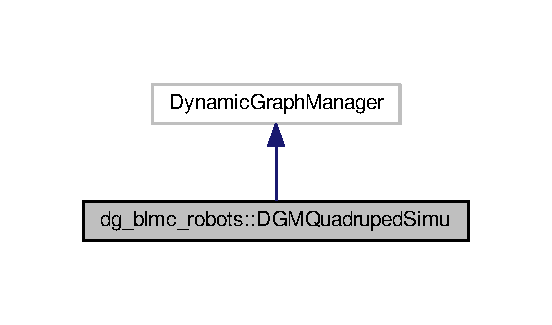
\includegraphics[width=265pt]{classdg__blmc__robots_1_1DGMQuadrupedSimu__inherit__graph}
\end{center}
\end{figure}


Collaboration diagram for dg\+\_\+blmc\+\_\+robots\+:\+:D\+G\+M\+Quadruped\+Simu\+:
\nopagebreak
\begin{figure}[H]
\begin{center}
\leavevmode
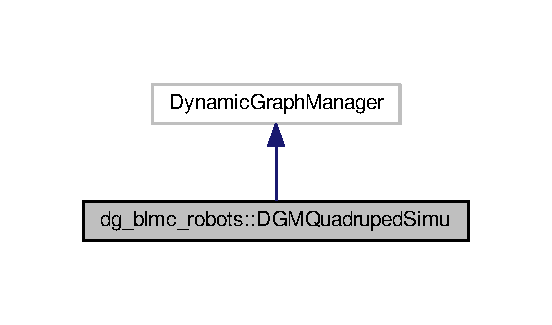
\includegraphics[width=265pt]{classdg__blmc__robots_1_1DGMQuadrupedSimu__coll__graph}
\end{center}
\end{figure}
\subsection*{Public Member Functions}
\begin{DoxyCompactItemize}
\item 
\hyperlink{classdg__blmc__robots_1_1DGMQuadrupedSimu_a6dd0768f9887c92a9fe26839b73771a3}{D\+G\+M\+Quadruped\+Simu} ()\hypertarget{classdg__blmc__robots_1_1DGMQuadrupedSimu_a6dd0768f9887c92a9fe26839b73771a3}{}\label{classdg__blmc__robots_1_1DGMQuadrupedSimu_a6dd0768f9887c92a9fe26839b73771a3}

\begin{DoxyCompactList}\small\item\em Demo\+Single\+Motor is the constructor. \end{DoxyCompactList}\item 
\hyperlink{classdg__blmc__robots_1_1DGMQuadrupedSimu_a5aabe831d173f9fc58c420b0ba33330f}{$\sim$\+D\+G\+M\+Quadruped\+Simu} ()\hypertarget{classdg__blmc__robots_1_1DGMQuadrupedSimu_a5aabe831d173f9fc58c420b0ba33330f}{}\label{classdg__blmc__robots_1_1DGMQuadrupedSimu_a5aabe831d173f9fc58c420b0ba33330f}

\begin{DoxyCompactList}\small\item\em $\sim$\+Demo\+Single\+Motor is the destructor. \end{DoxyCompactList}\item 
bool \hyperlink{classdg__blmc__robots_1_1DGMQuadrupedSimu_a89ae101b6a85455885d2ef9d7441941c}{is\+\_\+in\+\_\+safety\+\_\+mode} ()\hypertarget{classdg__blmc__robots_1_1DGMQuadrupedSimu_a89ae101b6a85455885d2ef9d7441941c}{}\label{classdg__blmc__robots_1_1DGMQuadrupedSimu_a89ae101b6a85455885d2ef9d7441941c}

\begin{DoxyCompactList}\small\item\em This function make also sure that the joint velocity do not exceed a certain value. \end{DoxyCompactList}\item 
void \hyperlink{classdg__blmc__robots_1_1DGMQuadrupedSimu_a1a5010a4279e2118c6d500427a223d07}{initialize\+\_\+hardware\+\_\+communication\+\_\+process} ()\hypertarget{classdg__blmc__robots_1_1DGMQuadrupedSimu_a1a5010a4279e2118c6d500427a223d07}{}\label{classdg__blmc__robots_1_1DGMQuadrupedSimu_a1a5010a4279e2118c6d500427a223d07}

\begin{DoxyCompactList}\small\item\em initialize\+\_\+hardware\+\_\+communication\+\_\+process is the function that initialize the hardware. \end{DoxyCompactList}\item 
void \hyperlink{classdg__blmc__robots_1_1DGMQuadrupedSimu_a6804388dddf35aa3980ec87c44606a14}{get\+\_\+sensors\+\_\+to\+\_\+map} (dynamic\+\_\+graph\+::\+Vector\+D\+G\+Map \&map)
\begin{DoxyCompactList}\small\item\em get\+\_\+sensors\+\_\+to\+\_\+map acquieres the sensors data and feed it to the input/output map \end{DoxyCompactList}\item 
void \hyperlink{classdg__blmc__robots_1_1DGMQuadrupedSimu_a431bbaae92470e69562c2749e35a75c8}{set\+\_\+motor\+\_\+controls\+\_\+from\+\_\+map} (const dynamic\+\_\+graph\+::\+Vector\+D\+G\+Map \&map)
\begin{DoxyCompactList}\small\item\em set\+\_\+motor\+\_\+controls\+\_\+from\+\_\+map reads the input map that contains the controls and send these controls to the hardware. \end{DoxyCompactList}\end{DoxyCompactItemize}
\subsection*{Private Attributes}
\begin{DoxyCompactItemize}
\item 
Vector8d \hyperlink{classdg__blmc__robots_1_1DGMQuadrupedSimu_a664b79890bc32dca86e185d09f8aafc4}{motor\+\_\+target\+\_\+currents\+\_\+}\hypertarget{classdg__blmc__robots_1_1DGMQuadrupedSimu_a664b79890bc32dca86e185d09f8aafc4}{}\label{classdg__blmc__robots_1_1DGMQuadrupedSimu_a664b79890bc32dca86e185d09f8aafc4}

\begin{DoxyCompactList}\small\item\em Entries for the simulated hardware. \end{DoxyCompactList}\item 
Vector8d {\bfseries motor\+\_\+torques\+\_\+}\hypertarget{classdg__blmc__robots_1_1DGMQuadrupedSimu_a3ca3d36a87cc6efcba595195bdba99c7}{}\label{classdg__blmc__robots_1_1DGMQuadrupedSimu_a3ca3d36a87cc6efcba595195bdba99c7}

\item 
Vector8d {\bfseries motor\+\_\+target\+\_\+torques\+\_\+}\hypertarget{classdg__blmc__robots_1_1DGMQuadrupedSimu_af5a7c4baa3e920227f0123fc907e12dd}{}\label{classdg__blmc__robots_1_1DGMQuadrupedSimu_af5a7c4baa3e920227f0123fc907e12dd}

\item 
Vector8d {\bfseries motor\+\_\+encoder\+\_\+indexes\+\_\+}\hypertarget{classdg__blmc__robots_1_1DGMQuadrupedSimu_abf4a5707075edfd128f4f3adced432b4}{}\label{classdg__blmc__robots_1_1DGMQuadrupedSimu_abf4a5707075edfd128f4f3adced432b4}

\item 
Vector8d {\bfseries joint\+\_\+positions\+\_\+}\hypertarget{classdg__blmc__robots_1_1DGMQuadrupedSimu_aa3df5cbb9c1305dd00083bae979308b4}{}\label{classdg__blmc__robots_1_1DGMQuadrupedSimu_aa3df5cbb9c1305dd00083bae979308b4}

\item 
Vector8d {\bfseries joint\+\_\+velocities\+\_\+}\hypertarget{classdg__blmc__robots_1_1DGMQuadrupedSimu_a0339ab56e226bb44358fd859bb451546}{}\label{classdg__blmc__robots_1_1DGMQuadrupedSimu_a0339ab56e226bb44358fd859bb451546}

\item 
Vector8d {\bfseries joint\+\_\+torques\+\_\+}\hypertarget{classdg__blmc__robots_1_1DGMQuadrupedSimu_a955e295bd749e25807c77d4a649ccd69}{}\label{classdg__blmc__robots_1_1DGMQuadrupedSimu_a955e295bd749e25807c77d4a649ccd69}

\item 
Vector8d {\bfseries joint\+\_\+target\+\_\+torques\+\_\+}\hypertarget{classdg__blmc__robots_1_1DGMQuadrupedSimu_a93819bd1ecaeb691d533acb443fe185f}{}\label{classdg__blmc__robots_1_1DGMQuadrupedSimu_a93819bd1ecaeb691d533acb443fe185f}

\item 
Vector4d {\bfseries contact\+\_\+sensors\+\_\+}\hypertarget{classdg__blmc__robots_1_1DGMQuadrupedSimu_a1db56af78a0fcb48da954e2a89afefe5}{}\label{classdg__blmc__robots_1_1DGMQuadrupedSimu_a1db56af78a0fcb48da954e2a89afefe5}

\item 
Vector4d {\bfseries slider\+\_\+positions\+\_\+}\hypertarget{classdg__blmc__robots_1_1DGMQuadrupedSimu_a15f06f8d2c4c1a890f361ed9bf25c5e6}{}\label{classdg__blmc__robots_1_1DGMQuadrupedSimu_a15f06f8d2c4c1a890f361ed9bf25c5e6}

\item 
Vector8d {\bfseries motor\+\_\+enabled\+\_\+}\hypertarget{classdg__blmc__robots_1_1DGMQuadrupedSimu_a3ca5fd3129cb1c400908ae3e9bc4717d}{}\label{classdg__blmc__robots_1_1DGMQuadrupedSimu_a3ca5fd3129cb1c400908ae3e9bc4717d}

\item 
Vector8d {\bfseries motor\+\_\+ready\+\_\+}\hypertarget{classdg__blmc__robots_1_1DGMQuadrupedSimu_a82e1782f8a9d28558be935c820978bf9}{}\label{classdg__blmc__robots_1_1DGMQuadrupedSimu_a82e1782f8a9d28558be935c820978bf9}

\item 
Vector4d {\bfseries motor\+\_\+board\+\_\+enabled\+\_\+}\hypertarget{classdg__blmc__robots_1_1DGMQuadrupedSimu_accc0e2374788ce5e6d13e641c2a86900}{}\label{classdg__blmc__robots_1_1DGMQuadrupedSimu_accc0e2374788ce5e6d13e641c2a86900}

\item 
Vector4d {\bfseries motor\+\_\+board\+\_\+errors\+\_\+}\hypertarget{classdg__blmc__robots_1_1DGMQuadrupedSimu_abcb00d4ab13ef169b4b7efa8a98f7a40}{}\label{classdg__blmc__robots_1_1DGMQuadrupedSimu_abcb00d4ab13ef169b4b7efa8a98f7a40}

\item 
Vector8d {\bfseries ctrl\+\_\+joint\+\_\+torques\+\_\+}\hypertarget{classdg__blmc__robots_1_1DGMQuadrupedSimu_a0a4ed493d2899823945cf1eceb8c3a9e}{}\label{classdg__blmc__robots_1_1DGMQuadrupedSimu_a0a4ed493d2899823945cf1eceb8c3a9e}

\item 
double {\bfseries motors\+\_\+inertia\+\_\+}\hypertarget{classdg__blmc__robots_1_1DGMQuadrupedSimu_a6be1446e66ba0553984b0c683b7ce74d}{}\label{classdg__blmc__robots_1_1DGMQuadrupedSimu_a6be1446e66ba0553984b0c683b7ce74d}

\item 
double {\bfseries motors\+\_\+torque\+\_\+constant\+\_\+}\hypertarget{classdg__blmc__robots_1_1DGMQuadrupedSimu_a341d34d4379a57de2f015862f25d54f6}{}\label{classdg__blmc__robots_1_1DGMQuadrupedSimu_a341d34d4379a57de2f015862f25d54f6}

\item 
double {\bfseries motors\+\_\+gear\+\_\+ratio\+\_\+}\hypertarget{classdg__blmc__robots_1_1DGMQuadrupedSimu_a95b261bc63aa641b5c416c1d64e39454}{}\label{classdg__blmc__robots_1_1DGMQuadrupedSimu_a95b261bc63aa641b5c416c1d64e39454}

\end{DoxyCompactItemize}


\subsection{Member Function Documentation}
\index{dg\+\_\+blmc\+\_\+robots\+::\+D\+G\+M\+Quadruped\+Simu@{dg\+\_\+blmc\+\_\+robots\+::\+D\+G\+M\+Quadruped\+Simu}!get\+\_\+sensors\+\_\+to\+\_\+map@{get\+\_\+sensors\+\_\+to\+\_\+map}}
\index{get\+\_\+sensors\+\_\+to\+\_\+map@{get\+\_\+sensors\+\_\+to\+\_\+map}!dg\+\_\+blmc\+\_\+robots\+::\+D\+G\+M\+Quadruped\+Simu@{dg\+\_\+blmc\+\_\+robots\+::\+D\+G\+M\+Quadruped\+Simu}}
\subsubsection[{\texorpdfstring{get\+\_\+sensors\+\_\+to\+\_\+map(dynamic\+\_\+graph\+::\+Vector\+D\+G\+Map \&map)}{get_sensors_to_map(dynamic_graph::VectorDGMap &map)}}]{\setlength{\rightskip}{0pt plus 5cm}void dg\+\_\+blmc\+\_\+robots\+::\+D\+G\+M\+Quadruped\+Simu\+::get\+\_\+sensors\+\_\+to\+\_\+map (
\begin{DoxyParamCaption}
\item[{dynamic\+\_\+graph\+::\+Vector\+D\+G\+Map \&}]{map}
\end{DoxyParamCaption}
)}\hypertarget{classdg__blmc__robots_1_1DGMQuadrupedSimu_a6804388dddf35aa3980ec87c44606a14}{}\label{classdg__blmc__robots_1_1DGMQuadrupedSimu_a6804388dddf35aa3980ec87c44606a14}


get\+\_\+sensors\+\_\+to\+\_\+map acquieres the sensors data and feed it to the input/output map 


\begin{DoxyParams}[1]{Parameters}
\mbox{\tt in}  & {\em } & \\
\hline
\end{DoxyParams}
\index{dg\+\_\+blmc\+\_\+robots\+::\+D\+G\+M\+Quadruped\+Simu@{dg\+\_\+blmc\+\_\+robots\+::\+D\+G\+M\+Quadruped\+Simu}!set\+\_\+motor\+\_\+controls\+\_\+from\+\_\+map@{set\+\_\+motor\+\_\+controls\+\_\+from\+\_\+map}}
\index{set\+\_\+motor\+\_\+controls\+\_\+from\+\_\+map@{set\+\_\+motor\+\_\+controls\+\_\+from\+\_\+map}!dg\+\_\+blmc\+\_\+robots\+::\+D\+G\+M\+Quadruped\+Simu@{dg\+\_\+blmc\+\_\+robots\+::\+D\+G\+M\+Quadruped\+Simu}}
\subsubsection[{\texorpdfstring{set\+\_\+motor\+\_\+controls\+\_\+from\+\_\+map(const dynamic\+\_\+graph\+::\+Vector\+D\+G\+Map \&map)}{set_motor_controls_from_map(const dynamic_graph::VectorDGMap &map)}}]{\setlength{\rightskip}{0pt plus 5cm}void dg\+\_\+blmc\+\_\+robots\+::\+D\+G\+M\+Quadruped\+Simu\+::set\+\_\+motor\+\_\+controls\+\_\+from\+\_\+map (
\begin{DoxyParamCaption}
\item[{const dynamic\+\_\+graph\+::\+Vector\+D\+G\+Map \&}]{map}
\end{DoxyParamCaption}
)}\hypertarget{classdg__blmc__robots_1_1DGMQuadrupedSimu_a431bbaae92470e69562c2749e35a75c8}{}\label{classdg__blmc__robots_1_1DGMQuadrupedSimu_a431bbaae92470e69562c2749e35a75c8}


set\+\_\+motor\+\_\+controls\+\_\+from\+\_\+map reads the input map that contains the controls and send these controls to the hardware. 


\begin{DoxyParams}{Parameters}
{\em map} & \\
\hline
\end{DoxyParams}


The documentation for this class was generated from the following files\+:\begin{DoxyCompactItemize}
\item 
include/dg\+\_\+blmc\+\_\+robots/dgm\+\_\+solo\+\_\+simple\+\_\+simu.\+hpp\item 
src/\hyperlink{dgm__solo__simple__simu_8cpp}{dgm\+\_\+solo\+\_\+simple\+\_\+simu.\+cpp}\end{DoxyCompactItemize}

\hypertarget{classdg__blmc__robots_1_1DGMSingleMotor}{}\section{dg\+\_\+blmc\+\_\+robots\+:\+:D\+G\+M\+Single\+Motor Class Reference}
\label{classdg__blmc__robots_1_1DGMSingleMotor}\index{dg\+\_\+blmc\+\_\+robots\+::\+D\+G\+M\+Single\+Motor@{dg\+\_\+blmc\+\_\+robots\+::\+D\+G\+M\+Single\+Motor}}


Inheritance diagram for dg\+\_\+blmc\+\_\+robots\+:\+:D\+G\+M\+Single\+Motor\+:
\nopagebreak
\begin{figure}[H]
\begin{center}
\leavevmode
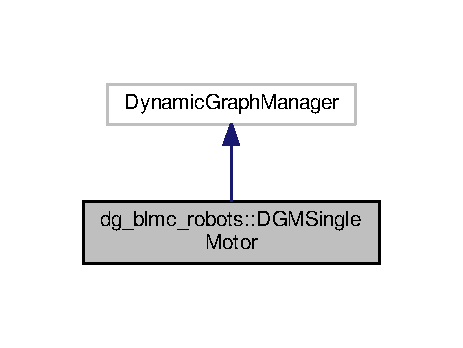
\includegraphics[width=222pt]{classdg__blmc__robots_1_1DGMSingleMotor__inherit__graph}
\end{center}
\end{figure}


Collaboration diagram for dg\+\_\+blmc\+\_\+robots\+:\+:D\+G\+M\+Single\+Motor\+:
\nopagebreak
\begin{figure}[H]
\begin{center}
\leavevmode
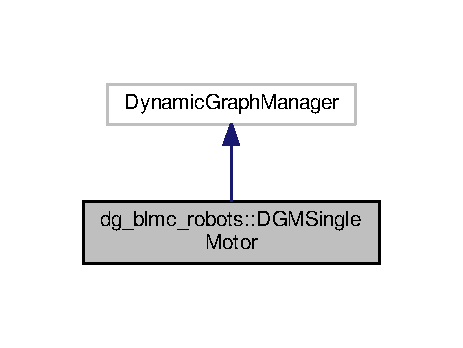
\includegraphics[width=222pt]{classdg__blmc__robots_1_1DGMSingleMotor__coll__graph}
\end{center}
\end{figure}
\subsection*{Public Member Functions}
\begin{DoxyCompactItemize}
\item 
\hyperlink{classdg__blmc__robots_1_1DGMSingleMotor_a3b2a7165e988dd54315ae47fede7f621}{D\+G\+M\+Single\+Motor} ()\hypertarget{classdg__blmc__robots_1_1DGMSingleMotor_a3b2a7165e988dd54315ae47fede7f621}{}\label{classdg__blmc__robots_1_1DGMSingleMotor_a3b2a7165e988dd54315ae47fede7f621}

\begin{DoxyCompactList}\small\item\em \hyperlink{classdg__blmc__robots_1_1DGMSingleMotor}{D\+G\+M\+Single\+Motor} is the constructor. \end{DoxyCompactList}\item 
\hyperlink{classdg__blmc__robots_1_1DGMSingleMotor_affcf3def46050538d1b84f310843a29a}{$\sim$\+D\+G\+M\+Single\+Motor} ()\hypertarget{classdg__blmc__robots_1_1DGMSingleMotor_affcf3def46050538d1b84f310843a29a}{}\label{classdg__blmc__robots_1_1DGMSingleMotor_affcf3def46050538d1b84f310843a29a}

\begin{DoxyCompactList}\small\item\em $\sim$\+D\+G\+M\+Single\+Motor is the destructor. \end{DoxyCompactList}\item 
void \hyperlink{classdg__blmc__robots_1_1DGMSingleMotor_af24b10d315284b3cf36a78155b193001}{initialize\+\_\+hardware\+\_\+communication\+\_\+process} ()\hypertarget{classdg__blmc__robots_1_1DGMSingleMotor_af24b10d315284b3cf36a78155b193001}{}\label{classdg__blmc__robots_1_1DGMSingleMotor_af24b10d315284b3cf36a78155b193001}

\begin{DoxyCompactList}\small\item\em initialize\+\_\+hardware\+\_\+communication\+\_\+process is the function that initialize the hardware. \end{DoxyCompactList}\item 
void \hyperlink{classdg__blmc__robots_1_1DGMSingleMotor_af7af9d26046e101fcdbab65507004a48}{get\+\_\+sensors\+\_\+to\+\_\+map} (dynamic\+\_\+graph\+::\+Vector\+D\+G\+Map \&map)
\begin{DoxyCompactList}\small\item\em get\+\_\+sensors\+\_\+to\+\_\+map acquires the sensors data and feed it to the input/output map \end{DoxyCompactList}\item 
void \hyperlink{classdg__blmc__robots_1_1DGMSingleMotor_a98bc6c87faf9121ef5fa7f1ba421d63e}{set\+\_\+motor\+\_\+controls\+\_\+from\+\_\+map} (const dynamic\+\_\+graph\+::\+Vector\+D\+G\+Map \&map)
\begin{DoxyCompactList}\small\item\em set\+\_\+motor\+\_\+controls\+\_\+from\+\_\+map reads the input map that contains the controls and send these controls to the hardware. \end{DoxyCompactList}\end{DoxyCompactItemize}
\subsection*{Private Attributes}
\begin{DoxyCompactItemize}
\item 
blmc\+\_\+robots\+::\+Single\+Motor \hyperlink{classdg__blmc__robots_1_1DGMSingleMotor_abd548dc88f1ded74bafea823244de422}{single\+\_\+motor\+\_\+}
\begin{DoxyCompactList}\small\item\em Entries for the real hardware. \end{DoxyCompactList}\item 
Vector1d \hyperlink{classdg__blmc__robots_1_1DGMSingleMotor_a6c092a7682bf6511d68c86f4b0ba51ea}{ctrl\+\_\+joint\+\_\+torques\+\_\+}\hypertarget{classdg__blmc__robots_1_1DGMSingleMotor_a6c092a7682bf6511d68c86f4b0ba51ea}{}\label{classdg__blmc__robots_1_1DGMSingleMotor_a6c092a7682bf6511d68c86f4b0ba51ea}

\begin{DoxyCompactList}\small\item\em ctrl\+\_\+joint\+\_\+torques\+\_\+ the motor torque to be sent \end{DoxyCompactList}\item 
bool \hyperlink{classdg__blmc__robots_1_1DGMSingleMotor_af341e50979dab7f63f4cf9b27e3fd772}{was\+\_\+in\+\_\+safety\+\_\+mode\+\_\+}\hypertarget{classdg__blmc__robots_1_1DGMSingleMotor_af341e50979dab7f63f4cf9b27e3fd772}{}\label{classdg__blmc__robots_1_1DGMSingleMotor_af341e50979dab7f63f4cf9b27e3fd772}

\begin{DoxyCompactList}\small\item\em was\+\_\+in\+\_\+safety\+\_\+mode\+\_\+ Toggle to keep in safety mode once it was entered. \end{DoxyCompactList}\end{DoxyCompactItemize}


\subsection{Member Function Documentation}
\index{dg\+\_\+blmc\+\_\+robots\+::\+D\+G\+M\+Single\+Motor@{dg\+\_\+blmc\+\_\+robots\+::\+D\+G\+M\+Single\+Motor}!get\+\_\+sensors\+\_\+to\+\_\+map@{get\+\_\+sensors\+\_\+to\+\_\+map}}
\index{get\+\_\+sensors\+\_\+to\+\_\+map@{get\+\_\+sensors\+\_\+to\+\_\+map}!dg\+\_\+blmc\+\_\+robots\+::\+D\+G\+M\+Single\+Motor@{dg\+\_\+blmc\+\_\+robots\+::\+D\+G\+M\+Single\+Motor}}
\subsubsection[{\texorpdfstring{get\+\_\+sensors\+\_\+to\+\_\+map(dynamic\+\_\+graph\+::\+Vector\+D\+G\+Map \&map)}{get_sensors_to_map(dynamic_graph::VectorDGMap &map)}}]{\setlength{\rightskip}{0pt plus 5cm}void dg\+\_\+blmc\+\_\+robots\+::\+D\+G\+M\+Single\+Motor\+::get\+\_\+sensors\+\_\+to\+\_\+map (
\begin{DoxyParamCaption}
\item[{dynamic\+\_\+graph\+::\+Vector\+D\+G\+Map \&}]{map}
\end{DoxyParamCaption}
)}\hypertarget{classdg__blmc__robots_1_1DGMSingleMotor_af7af9d26046e101fcdbab65507004a48}{}\label{classdg__blmc__robots_1_1DGMSingleMotor_af7af9d26046e101fcdbab65507004a48}


get\+\_\+sensors\+\_\+to\+\_\+map acquires the sensors data and feed it to the input/output map 


\begin{DoxyParams}[1]{Parameters}
\mbox{\tt in}  & {\em } & \\
\hline
\end{DoxyParams}
\index{dg\+\_\+blmc\+\_\+robots\+::\+D\+G\+M\+Single\+Motor@{dg\+\_\+blmc\+\_\+robots\+::\+D\+G\+M\+Single\+Motor}!set\+\_\+motor\+\_\+controls\+\_\+from\+\_\+map@{set\+\_\+motor\+\_\+controls\+\_\+from\+\_\+map}}
\index{set\+\_\+motor\+\_\+controls\+\_\+from\+\_\+map@{set\+\_\+motor\+\_\+controls\+\_\+from\+\_\+map}!dg\+\_\+blmc\+\_\+robots\+::\+D\+G\+M\+Single\+Motor@{dg\+\_\+blmc\+\_\+robots\+::\+D\+G\+M\+Single\+Motor}}
\subsubsection[{\texorpdfstring{set\+\_\+motor\+\_\+controls\+\_\+from\+\_\+map(const dynamic\+\_\+graph\+::\+Vector\+D\+G\+Map \&map)}{set_motor_controls_from_map(const dynamic_graph::VectorDGMap &map)}}]{\setlength{\rightskip}{0pt plus 5cm}void dg\+\_\+blmc\+\_\+robots\+::\+D\+G\+M\+Single\+Motor\+::set\+\_\+motor\+\_\+controls\+\_\+from\+\_\+map (
\begin{DoxyParamCaption}
\item[{const dynamic\+\_\+graph\+::\+Vector\+D\+G\+Map \&}]{map}
\end{DoxyParamCaption}
)}\hypertarget{classdg__blmc__robots_1_1DGMSingleMotor_a98bc6c87faf9121ef5fa7f1ba421d63e}{}\label{classdg__blmc__robots_1_1DGMSingleMotor_a98bc6c87faf9121ef5fa7f1ba421d63e}


set\+\_\+motor\+\_\+controls\+\_\+from\+\_\+map reads the input map that contains the controls and send these controls to the hardware. 


\begin{DoxyParams}{Parameters}
{\em map} & \\
\hline
\end{DoxyParams}


\subsection{Member Data Documentation}
\index{dg\+\_\+blmc\+\_\+robots\+::\+D\+G\+M\+Single\+Motor@{dg\+\_\+blmc\+\_\+robots\+::\+D\+G\+M\+Single\+Motor}!single\+\_\+motor\+\_\+@{single\+\_\+motor\+\_\+}}
\index{single\+\_\+motor\+\_\+@{single\+\_\+motor\+\_\+}!dg\+\_\+blmc\+\_\+robots\+::\+D\+G\+M\+Single\+Motor@{dg\+\_\+blmc\+\_\+robots\+::\+D\+G\+M\+Single\+Motor}}
\subsubsection[{\texorpdfstring{single\+\_\+motor\+\_\+}{single_motor_}}]{\setlength{\rightskip}{0pt plus 5cm}blmc\+\_\+robots\+::\+Single\+Motor dg\+\_\+blmc\+\_\+robots\+::\+D\+G\+M\+Single\+Motor\+::single\+\_\+motor\+\_\+\hspace{0.3cm}{\ttfamily [private]}}\hypertarget{classdg__blmc__robots_1_1DGMSingleMotor_abd548dc88f1ded74bafea823244de422}{}\label{classdg__blmc__robots_1_1DGMSingleMotor_abd548dc88f1ded74bafea823244de422}


Entries for the real hardware. 

single\+\_\+motor\+\_\+ the real motor hardware drivers. 

The documentation for this class was generated from the following file\+:\begin{DoxyCompactItemize}
\item 
include/dg\+\_\+blmc\+\_\+robots/\hyperlink{dgm__single__motor_8hpp}{dgm\+\_\+single\+\_\+motor.\+hpp}\end{DoxyCompactItemize}

\hypertarget{classdg__blmc__robots_1_1DGMSolo12}{}\section{dg\+\_\+blmc\+\_\+robots\+:\+:D\+G\+M\+Solo12 Class Reference}
\label{classdg__blmc__robots_1_1DGMSolo12}\index{dg\+\_\+blmc\+\_\+robots\+::\+D\+G\+M\+Solo12@{dg\+\_\+blmc\+\_\+robots\+::\+D\+G\+M\+Solo12}}


Inheritance diagram for dg\+\_\+blmc\+\_\+robots\+:\+:D\+G\+M\+Solo12\+:
\nopagebreak
\begin{figure}[H]
\begin{center}
\leavevmode
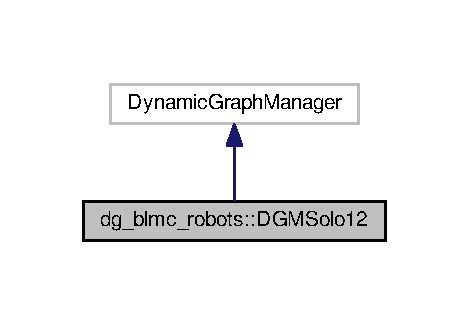
\includegraphics[width=225pt]{classdg__blmc__robots_1_1DGMSolo12__inherit__graph}
\end{center}
\end{figure}


Collaboration diagram for dg\+\_\+blmc\+\_\+robots\+:\+:D\+G\+M\+Solo12\+:
\nopagebreak
\begin{figure}[H]
\begin{center}
\leavevmode
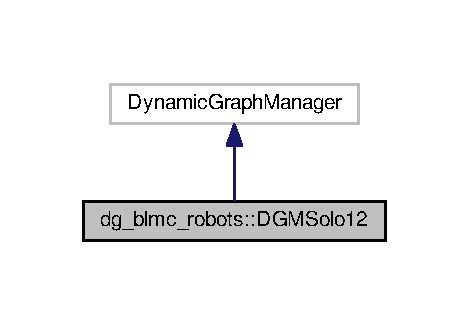
\includegraphics[width=225pt]{classdg__blmc__robots_1_1DGMSolo12__coll__graph}
\end{center}
\end{figure}
\subsection*{Public Member Functions}
\begin{DoxyCompactItemize}
\item 
\hyperlink{classdg__blmc__robots_1_1DGMSolo12_af723971f57c6acb3168aa08876e3798e}{D\+G\+M\+Solo12} ()\hypertarget{classdg__blmc__robots_1_1DGMSolo12_af723971f57c6acb3168aa08876e3798e}{}\label{classdg__blmc__robots_1_1DGMSolo12_af723971f57c6acb3168aa08876e3798e}

\begin{DoxyCompactList}\small\item\em Demo\+Single\+Motor is the constructor. \end{DoxyCompactList}\item 
\hyperlink{classdg__blmc__robots_1_1DGMSolo12_a1e3ebce3491c53013e089883393c3338}{$\sim$\+D\+G\+M\+Solo12} ()\hypertarget{classdg__blmc__robots_1_1DGMSolo12_a1e3ebce3491c53013e089883393c3338}{}\label{classdg__blmc__robots_1_1DGMSolo12_a1e3ebce3491c53013e089883393c3338}

\begin{DoxyCompactList}\small\item\em $\sim$\+Demo\+Single\+Motor is the destructor. \end{DoxyCompactList}\item 
bool \hyperlink{classdg__blmc__robots_1_1DGMSolo12_aa6302b840e6e3c86b9fc4d9bf05a21ef}{is\+\_\+in\+\_\+safety\+\_\+mode} ()\hypertarget{classdg__blmc__robots_1_1DGMSolo12_aa6302b840e6e3c86b9fc4d9bf05a21ef}{}\label{classdg__blmc__robots_1_1DGMSolo12_aa6302b840e6e3c86b9fc4d9bf05a21ef}

\begin{DoxyCompactList}\small\item\em This function make also sure that the joint velocity do not exceed a certain value. \end{DoxyCompactList}\item 
void \hyperlink{classdg__blmc__robots_1_1DGMSolo12_a4d5af277b58accfedcadbac524b23efc}{initialize\+\_\+hardware\+\_\+communication\+\_\+process} ()
\begin{DoxyCompactList}\small\item\em initialize\+\_\+hardware\+\_\+communication\+\_\+process is the function that initialize the hardware. \end{DoxyCompactList}\item 
void \hyperlink{classdg__blmc__robots_1_1DGMSolo12_a407925fdfb633e0bfab911c90ca01c04}{get\+\_\+sensors\+\_\+to\+\_\+map} (dynamic\+\_\+graph\+::\+Vector\+D\+G\+Map \&map)
\begin{DoxyCompactList}\small\item\em get\+\_\+sensors\+\_\+to\+\_\+map acquieres the sensors data and feed it to the input/output map \end{DoxyCompactList}\item 
void \hyperlink{classdg__blmc__robots_1_1DGMSolo12_a8e7ed8c9ee0a69f3370c502ccf47d9c9}{set\+\_\+motor\+\_\+controls\+\_\+from\+\_\+map} (const dynamic\+\_\+graph\+::\+Vector\+D\+G\+Map \&map)
\begin{DoxyCompactList}\small\item\em set\+\_\+motor\+\_\+controls\+\_\+from\+\_\+map reads the input map that contains the controls and send these controls to the hardware. \end{DoxyCompactList}\item 
bool \hyperlink{classdg__blmc__robots_1_1DGMSolo12_af261744a5d36308874dc08d660711280}{calibrate\+\_\+joint\+\_\+position\+\_\+callback} (dg\+\_\+blmc\+\_\+robots\+::\+Joint\+Calibration\+::\+Request \&req, dg\+\_\+blmc\+\_\+robots\+::\+Joint\+Calibration\+::\+Response \&res)
\begin{DoxyCompactList}\small\item\em Ros callback for the callibration procedure. \end{DoxyCompactList}\end{DoxyCompactItemize}
\subsection*{Private Member Functions}
\begin{DoxyCompactItemize}
\item 
void \hyperlink{classdg__blmc__robots_1_1DGMSolo12_a63196391c1aee97f94c8c2f3a66b4a0b}{calibrate\+\_\+joint\+\_\+position} (const blmc\+\_\+robots\+::\+Vector12d \&zero\+\_\+to\+\_\+index\+\_\+angle)
\begin{DoxyCompactList}\small\item\em Calibrate the robot joint position. \end{DoxyCompactList}\end{DoxyCompactItemize}
\subsection*{Private Attributes}
\begin{DoxyCompactItemize}
\item 
blmc\+\_\+robots\+::\+Solo12 \hyperlink{classdg__blmc__robots_1_1DGMSolo12_a7c8edf5752598bafc7cd33380910e5ae}{solo\+\_\+}
\begin{DoxyCompactList}\small\item\em Entries for the real hardware. \end{DoxyCompactList}\item 
blmc\+\_\+robots\+::\+Vector12d \hyperlink{classdg__blmc__robots_1_1DGMSolo12_a8eaf78b77ea59bedbbcf23aabcdd66e0}{ctrl\+\_\+joint\+\_\+torques\+\_\+}
\begin{DoxyCompactList}\small\item\em ctrl\+\_\+joint\+\_\+torques\+\_\+ the joint torques to be sent. \end{DoxyCompactList}\item 
bool \hyperlink{classdg__blmc__robots_1_1DGMSolo12_a2a5156d24e66e1af93bc94f5f03ccb67}{was\+\_\+in\+\_\+safety\+\_\+mode\+\_\+}\hypertarget{classdg__blmc__robots_1_1DGMSolo12_a2a5156d24e66e1af93bc94f5f03ccb67}{}\label{classdg__blmc__robots_1_1DGMSolo12_a2a5156d24e66e1af93bc94f5f03ccb67}

\begin{DoxyCompactList}\small\item\em Check if we entered once in the safety mode and stay there if so. \end{DoxyCompactList}\item 
blmc\+\_\+robots\+::\+Vector12d \hyperlink{classdg__blmc__robots_1_1DGMSolo12_abb9b4edf8c97cfecbaf87b6adaad8ad5}{zero\+\_\+to\+\_\+index\+\_\+angle\+\_\+from\+\_\+file\+\_\+}
\begin{DoxyCompactList}\small\item\em These are the calibration value extracted from the paramters. \end{DoxyCompactList}\end{DoxyCompactItemize}


\subsection{Member Function Documentation}
\index{dg\+\_\+blmc\+\_\+robots\+::\+D\+G\+M\+Solo12@{dg\+\_\+blmc\+\_\+robots\+::\+D\+G\+M\+Solo12}!calibrate\+\_\+joint\+\_\+position@{calibrate\+\_\+joint\+\_\+position}}
\index{calibrate\+\_\+joint\+\_\+position@{calibrate\+\_\+joint\+\_\+position}!dg\+\_\+blmc\+\_\+robots\+::\+D\+G\+M\+Solo12@{dg\+\_\+blmc\+\_\+robots\+::\+D\+G\+M\+Solo12}}
\subsubsection[{\texorpdfstring{calibrate\+\_\+joint\+\_\+position(const blmc\+\_\+robots\+::\+Vector12d \&zero\+\_\+to\+\_\+index\+\_\+angle)}{calibrate_joint_position(const blmc_robots::Vector12d &zero_to_index_angle)}}]{\setlength{\rightskip}{0pt plus 5cm}void dg\+\_\+blmc\+\_\+robots\+::\+D\+G\+M\+Solo12\+::calibrate\+\_\+joint\+\_\+position (
\begin{DoxyParamCaption}
\item[{const blmc\+\_\+robots\+::\+Vector12d \&}]{zero\+\_\+to\+\_\+index\+\_\+angle}
\end{DoxyParamCaption}
)\hspace{0.3cm}{\ttfamily [private]}}\hypertarget{classdg__blmc__robots_1_1DGMSolo12_a63196391c1aee97f94c8c2f3a66b4a0b}{}\label{classdg__blmc__robots_1_1DGMSolo12_a63196391c1aee97f94c8c2f3a66b4a0b}


Calibrate the robot joint position. 


\begin{DoxyParams}{Parameters}
{\em zero\+\_\+to\+\_\+index\+\_\+angle} & is the angle between the theoretical zero and the next positive angle. \\
\hline
\end{DoxyParams}
\index{dg\+\_\+blmc\+\_\+robots\+::\+D\+G\+M\+Solo12@{dg\+\_\+blmc\+\_\+robots\+::\+D\+G\+M\+Solo12}!calibrate\+\_\+joint\+\_\+position\+\_\+callback@{calibrate\+\_\+joint\+\_\+position\+\_\+callback}}
\index{calibrate\+\_\+joint\+\_\+position\+\_\+callback@{calibrate\+\_\+joint\+\_\+position\+\_\+callback}!dg\+\_\+blmc\+\_\+robots\+::\+D\+G\+M\+Solo12@{dg\+\_\+blmc\+\_\+robots\+::\+D\+G\+M\+Solo12}}
\subsubsection[{\texorpdfstring{calibrate\+\_\+joint\+\_\+position\+\_\+callback(dg\+\_\+blmc\+\_\+robots\+::\+Joint\+Calibration\+::\+Request \&req, dg\+\_\+blmc\+\_\+robots\+::\+Joint\+Calibration\+::\+Response \&res)}{calibrate_joint_position_callback(dg_blmc_robots::JointCalibration::Request &req, dg_blmc_robots::JointCalibration::Response &res)}}]{\setlength{\rightskip}{0pt plus 5cm}bool dg\+\_\+blmc\+\_\+robots\+::\+D\+G\+M\+Solo12\+::calibrate\+\_\+joint\+\_\+position\+\_\+callback (
\begin{DoxyParamCaption}
\item[{dg\+\_\+blmc\+\_\+robots\+::\+Joint\+Calibration\+::\+Request \&}]{req, }
\item[{dg\+\_\+blmc\+\_\+robots\+::\+Joint\+Calibration\+::\+Response \&}]{res}
\end{DoxyParamCaption}
)}\hypertarget{classdg__blmc__robots_1_1DGMSolo12_af261744a5d36308874dc08d660711280}{}\label{classdg__blmc__robots_1_1DGMSolo12_af261744a5d36308874dc08d660711280}


Ros callback for the callibration procedure. 

Warning the robot will move to the next the joint index and back to \char`\"{}0\char`\"{} upon this call. Be sure that no controller are running in parallel.


\begin{DoxyParams}{Parameters}
{\em req} & nothing \\
\hline
{\em res} & True if everything went well. \\
\hline
\end{DoxyParams}
\begin{DoxyReturn}{Returns}
true if everything went well. 

false if something went wrong. 
\end{DoxyReturn}
\index{dg\+\_\+blmc\+\_\+robots\+::\+D\+G\+M\+Solo12@{dg\+\_\+blmc\+\_\+robots\+::\+D\+G\+M\+Solo12}!get\+\_\+sensors\+\_\+to\+\_\+map@{get\+\_\+sensors\+\_\+to\+\_\+map}}
\index{get\+\_\+sensors\+\_\+to\+\_\+map@{get\+\_\+sensors\+\_\+to\+\_\+map}!dg\+\_\+blmc\+\_\+robots\+::\+D\+G\+M\+Solo12@{dg\+\_\+blmc\+\_\+robots\+::\+D\+G\+M\+Solo12}}
\subsubsection[{\texorpdfstring{get\+\_\+sensors\+\_\+to\+\_\+map(dynamic\+\_\+graph\+::\+Vector\+D\+G\+Map \&map)}{get_sensors_to_map(dynamic_graph::VectorDGMap &map)}}]{\setlength{\rightskip}{0pt plus 5cm}void dg\+\_\+blmc\+\_\+robots\+::\+D\+G\+M\+Solo12\+::get\+\_\+sensors\+\_\+to\+\_\+map (
\begin{DoxyParamCaption}
\item[{dynamic\+\_\+graph\+::\+Vector\+D\+G\+Map \&}]{map}
\end{DoxyParamCaption}
)}\hypertarget{classdg__blmc__robots_1_1DGMSolo12_a407925fdfb633e0bfab911c90ca01c04}{}\label{classdg__blmc__robots_1_1DGMSolo12_a407925fdfb633e0bfab911c90ca01c04}


get\+\_\+sensors\+\_\+to\+\_\+map acquieres the sensors data and feed it to the input/output map 


\begin{DoxyParams}[1]{Parameters}
\mbox{\tt in}  & {\em } & \\
\hline
\end{DoxyParams}
Joint data.

Additional data.

Robot status.\index{dg\+\_\+blmc\+\_\+robots\+::\+D\+G\+M\+Solo12@{dg\+\_\+blmc\+\_\+robots\+::\+D\+G\+M\+Solo12}!initialize\+\_\+hardware\+\_\+communication\+\_\+process@{initialize\+\_\+hardware\+\_\+communication\+\_\+process}}
\index{initialize\+\_\+hardware\+\_\+communication\+\_\+process@{initialize\+\_\+hardware\+\_\+communication\+\_\+process}!dg\+\_\+blmc\+\_\+robots\+::\+D\+G\+M\+Solo12@{dg\+\_\+blmc\+\_\+robots\+::\+D\+G\+M\+Solo12}}
\subsubsection[{\texorpdfstring{initialize\+\_\+hardware\+\_\+communication\+\_\+process()}{initialize_hardware_communication_process()}}]{\setlength{\rightskip}{0pt plus 5cm}void dg\+\_\+blmc\+\_\+robots\+::\+D\+G\+M\+Solo12\+::initialize\+\_\+hardware\+\_\+communication\+\_\+process (
\begin{DoxyParamCaption}
{}
\end{DoxyParamCaption}
)}\hypertarget{classdg__blmc__robots_1_1DGMSolo12_a4d5af277b58accfedcadbac524b23efc}{}\label{classdg__blmc__robots_1_1DGMSolo12_a4d5af277b58accfedcadbac524b23efc}


initialize\+\_\+hardware\+\_\+communication\+\_\+process is the function that initialize the hardware. 

Load the calibration parameters.

Initialize the user commands. \index{dg\+\_\+blmc\+\_\+robots\+::\+D\+G\+M\+Solo12@{dg\+\_\+blmc\+\_\+robots\+::\+D\+G\+M\+Solo12}!set\+\_\+motor\+\_\+controls\+\_\+from\+\_\+map@{set\+\_\+motor\+\_\+controls\+\_\+from\+\_\+map}}
\index{set\+\_\+motor\+\_\+controls\+\_\+from\+\_\+map@{set\+\_\+motor\+\_\+controls\+\_\+from\+\_\+map}!dg\+\_\+blmc\+\_\+robots\+::\+D\+G\+M\+Solo12@{dg\+\_\+blmc\+\_\+robots\+::\+D\+G\+M\+Solo12}}
\subsubsection[{\texorpdfstring{set\+\_\+motor\+\_\+controls\+\_\+from\+\_\+map(const dynamic\+\_\+graph\+::\+Vector\+D\+G\+Map \&map)}{set_motor_controls_from_map(const dynamic_graph::VectorDGMap &map)}}]{\setlength{\rightskip}{0pt plus 5cm}void dg\+\_\+blmc\+\_\+robots\+::\+D\+G\+M\+Solo12\+::set\+\_\+motor\+\_\+controls\+\_\+from\+\_\+map (
\begin{DoxyParamCaption}
\item[{const dynamic\+\_\+graph\+::\+Vector\+D\+G\+Map \&}]{map}
\end{DoxyParamCaption}
)}\hypertarget{classdg__blmc__robots_1_1DGMSolo12_a8e7ed8c9ee0a69f3370c502ccf47d9c9}{}\label{classdg__blmc__robots_1_1DGMSolo12_a8e7ed8c9ee0a69f3370c502ccf47d9c9}


set\+\_\+motor\+\_\+controls\+\_\+from\+\_\+map reads the input map that contains the controls and send these controls to the hardware. 


\begin{DoxyParams}{Parameters}
{\em map} & \\
\hline
\end{DoxyParams}


\subsection{Member Data Documentation}
\index{dg\+\_\+blmc\+\_\+robots\+::\+D\+G\+M\+Solo12@{dg\+\_\+blmc\+\_\+robots\+::\+D\+G\+M\+Solo12}!ctrl\+\_\+joint\+\_\+torques\+\_\+@{ctrl\+\_\+joint\+\_\+torques\+\_\+}}
\index{ctrl\+\_\+joint\+\_\+torques\+\_\+@{ctrl\+\_\+joint\+\_\+torques\+\_\+}!dg\+\_\+blmc\+\_\+robots\+::\+D\+G\+M\+Solo12@{dg\+\_\+blmc\+\_\+robots\+::\+D\+G\+M\+Solo12}}
\subsubsection[{\texorpdfstring{ctrl\+\_\+joint\+\_\+torques\+\_\+}{ctrl_joint_torques_}}]{\setlength{\rightskip}{0pt plus 5cm}blmc\+\_\+robots\+::\+Vector12d dg\+\_\+blmc\+\_\+robots\+::\+D\+G\+M\+Solo12\+::ctrl\+\_\+joint\+\_\+torques\+\_\+\hspace{0.3cm}{\ttfamily [private]}}\hypertarget{classdg__blmc__robots_1_1DGMSolo12_a8eaf78b77ea59bedbbcf23aabcdd66e0}{}\label{classdg__blmc__robots_1_1DGMSolo12_a8eaf78b77ea59bedbbcf23aabcdd66e0}


ctrl\+\_\+joint\+\_\+torques\+\_\+ the joint torques to be sent. 

Used in this class to perform a local copy of the control. This is need in order to send this copy to the blmc\+\_\+robots\+::\+Solo class \index{dg\+\_\+blmc\+\_\+robots\+::\+D\+G\+M\+Solo12@{dg\+\_\+blmc\+\_\+robots\+::\+D\+G\+M\+Solo12}!solo\+\_\+@{solo\+\_\+}}
\index{solo\+\_\+@{solo\+\_\+}!dg\+\_\+blmc\+\_\+robots\+::\+D\+G\+M\+Solo12@{dg\+\_\+blmc\+\_\+robots\+::\+D\+G\+M\+Solo12}}
\subsubsection[{\texorpdfstring{solo\+\_\+}{solo_}}]{\setlength{\rightskip}{0pt plus 5cm}blmc\+\_\+robots\+::\+Solo12 dg\+\_\+blmc\+\_\+robots\+::\+D\+G\+M\+Solo12\+::solo\+\_\+\hspace{0.3cm}{\ttfamily [private]}}\hypertarget{classdg__blmc__robots_1_1DGMSolo12_a7c8edf5752598bafc7cd33380910e5ae}{}\label{classdg__blmc__robots_1_1DGMSolo12_a7c8edf5752598bafc7cd33380910e5ae}


Entries for the real hardware. 

test\+\_\+bench\+\_\+ the real test bench hardware drivers. \index{dg\+\_\+blmc\+\_\+robots\+::\+D\+G\+M\+Solo12@{dg\+\_\+blmc\+\_\+robots\+::\+D\+G\+M\+Solo12}!zero\+\_\+to\+\_\+index\+\_\+angle\+\_\+from\+\_\+file\+\_\+@{zero\+\_\+to\+\_\+index\+\_\+angle\+\_\+from\+\_\+file\+\_\+}}
\index{zero\+\_\+to\+\_\+index\+\_\+angle\+\_\+from\+\_\+file\+\_\+@{zero\+\_\+to\+\_\+index\+\_\+angle\+\_\+from\+\_\+file\+\_\+}!dg\+\_\+blmc\+\_\+robots\+::\+D\+G\+M\+Solo12@{dg\+\_\+blmc\+\_\+robots\+::\+D\+G\+M\+Solo12}}
\subsubsection[{\texorpdfstring{zero\+\_\+to\+\_\+index\+\_\+angle\+\_\+from\+\_\+file\+\_\+}{zero_to_index_angle_from_file_}}]{\setlength{\rightskip}{0pt plus 5cm}blmc\+\_\+robots\+::\+Vector12d dg\+\_\+blmc\+\_\+robots\+::\+D\+G\+M\+Solo12\+::zero\+\_\+to\+\_\+index\+\_\+angle\+\_\+from\+\_\+file\+\_\+\hspace{0.3cm}{\ttfamily [private]}}\hypertarget{classdg__blmc__robots_1_1DGMSolo12_abb9b4edf8c97cfecbaf87b6adaad8ad5}{}\label{classdg__blmc__robots_1_1DGMSolo12_abb9b4edf8c97cfecbaf87b6adaad8ad5}


These are the calibration value extracted from the paramters. 

They represent the distance between the theorical zero joint angle and the next jont index. 

The documentation for this class was generated from the following files\+:\begin{DoxyCompactItemize}
\item 
include/dg\+\_\+blmc\+\_\+robots/dgm\+\_\+solo12.\+hpp\item 
src/dgm\+\_\+solo12.\+cpp\end{DoxyCompactItemize}

\hypertarget{classdg__blmc__robots_1_1DGMSolo8}{}\section{dg\+\_\+blmc\+\_\+robots\+:\+:D\+G\+M\+Solo8 Class Reference}
\label{classdg__blmc__robots_1_1DGMSolo8}\index{dg\+\_\+blmc\+\_\+robots\+::\+D\+G\+M\+Solo8@{dg\+\_\+blmc\+\_\+robots\+::\+D\+G\+M\+Solo8}}


Inheritance diagram for dg\+\_\+blmc\+\_\+robots\+:\+:D\+G\+M\+Solo8\+:
\nopagebreak
\begin{figure}[H]
\begin{center}
\leavevmode
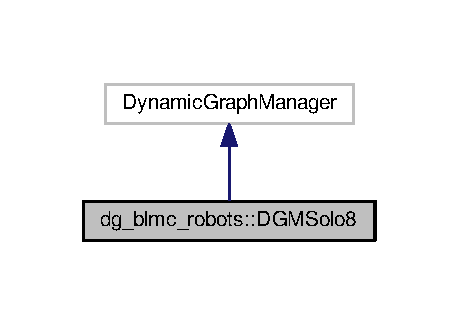
\includegraphics[width=220pt]{classdg__blmc__robots_1_1DGMSolo8__inherit__graph}
\end{center}
\end{figure}


Collaboration diagram for dg\+\_\+blmc\+\_\+robots\+:\+:D\+G\+M\+Solo8\+:
\nopagebreak
\begin{figure}[H]
\begin{center}
\leavevmode
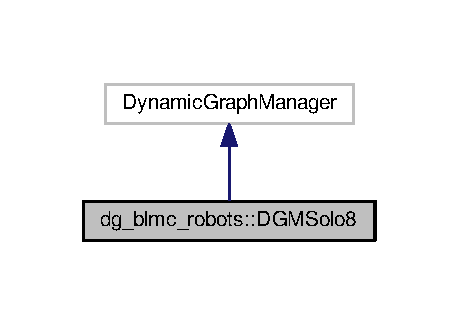
\includegraphics[width=220pt]{classdg__blmc__robots_1_1DGMSolo8__coll__graph}
\end{center}
\end{figure}
\subsection*{Public Member Functions}
\begin{DoxyCompactItemize}
\item 
\hyperlink{classdg__blmc__robots_1_1DGMSolo8_ac60de8a48c9fcf7d1f769dab90753e2b}{D\+G\+M\+Solo8} ()\hypertarget{classdg__blmc__robots_1_1DGMSolo8_ac60de8a48c9fcf7d1f769dab90753e2b}{}\label{classdg__blmc__robots_1_1DGMSolo8_ac60de8a48c9fcf7d1f769dab90753e2b}

\begin{DoxyCompactList}\small\item\em Demo\+Single\+Motor is the constructor. \end{DoxyCompactList}\item 
\hyperlink{classdg__blmc__robots_1_1DGMSolo8_a260d27a6376606bc72e07caf445435d2}{$\sim$\+D\+G\+M\+Solo8} ()\hypertarget{classdg__blmc__robots_1_1DGMSolo8_a260d27a6376606bc72e07caf445435d2}{}\label{classdg__blmc__robots_1_1DGMSolo8_a260d27a6376606bc72e07caf445435d2}

\begin{DoxyCompactList}\small\item\em $\sim$\+Demo\+Single\+Motor is the destructor. \end{DoxyCompactList}\item 
void \hyperlink{classdg__blmc__robots_1_1DGMSolo8_ac2d419f12dd51ea7cf5b429f766e21c2}{initialize\+\_\+hardware\+\_\+communication\+\_\+process} ()
\begin{DoxyCompactList}\small\item\em This function make also sure that the joint velocity do not exceed a certain value. \end{DoxyCompactList}\item 
void \hyperlink{classdg__blmc__robots_1_1DGMSolo8_a5c024946d27b7b52b3b6cc568efe96df}{get\+\_\+sensors\+\_\+to\+\_\+map} (dynamic\+\_\+graph\+::\+Vector\+D\+G\+Map \&map)
\begin{DoxyCompactList}\small\item\em get\+\_\+sensors\+\_\+to\+\_\+map acquieres the sensors data and feed it to the input/output map \end{DoxyCompactList}\item 
void \hyperlink{classdg__blmc__robots_1_1DGMSolo8_a7b6f7771158eada4f93cf5d156fbe9a9}{set\+\_\+motor\+\_\+controls\+\_\+from\+\_\+map} (const dynamic\+\_\+graph\+::\+Vector\+D\+G\+Map \&map)
\begin{DoxyCompactList}\small\item\em set\+\_\+motor\+\_\+controls\+\_\+from\+\_\+map reads the input map that contains the controls and send these controls to the hardware. \end{DoxyCompactList}\item 
bool \hyperlink{classdg__blmc__robots_1_1DGMSolo8_add051134152340a82e5466e186d15c0e}{calibrate\+\_\+joint\+\_\+position\+\_\+callback} (dg\+\_\+blmc\+\_\+robots\+::\+Joint\+Calibration\+::\+Request \&req, dg\+\_\+blmc\+\_\+robots\+::\+Joint\+Calibration\+::\+Response \&res)
\end{DoxyCompactItemize}
\subsection*{Private Member Functions}
\begin{DoxyCompactItemize}
\item 
void \hyperlink{classdg__blmc__robots_1_1DGMSolo8_adc94f7989828834b503739c51d4af3fe}{calibrate\+\_\+joint\+\_\+position} (const blmc\+\_\+robots\+::\+Vector8d \&zero\+\_\+to\+\_\+index\+\_\+angle)
\begin{DoxyCompactList}\small\item\em Calibrate the robot joint position. \end{DoxyCompactList}\end{DoxyCompactItemize}
\subsection*{Private Attributes}
\begin{DoxyCompactItemize}
\item 
blmc\+\_\+robots\+::\+Solo8 \hyperlink{classdg__blmc__robots_1_1DGMSolo8_a65ce342929838851ee3fe9f0f9633088}{solo\+\_\+}
\begin{DoxyCompactList}\small\item\em Entries for the real hardware. \end{DoxyCompactList}\item 
blmc\+\_\+robots\+::\+Vector8d \hyperlink{classdg__blmc__robots_1_1DGMSolo8_a81971c21240a172c936c56cdfbf0a02c}{ctrl\+\_\+joint\+\_\+torques\+\_\+}
\begin{DoxyCompactList}\small\item\em ctrl\+\_\+joint\+\_\+torques\+\_\+ the joint torques to be sent. \end{DoxyCompactList}\item 
bool \hyperlink{classdg__blmc__robots_1_1DGMSolo8_a4ab54e51e268880d3e34144fbb1ee7a5}{was\+\_\+in\+\_\+safety\+\_\+mode\+\_\+}\hypertarget{classdg__blmc__robots_1_1DGMSolo8_a4ab54e51e268880d3e34144fbb1ee7a5}{}\label{classdg__blmc__robots_1_1DGMSolo8_a4ab54e51e268880d3e34144fbb1ee7a5}

\begin{DoxyCompactList}\small\item\em Check if we entered once in the safety mode and stay there if so. \end{DoxyCompactList}\item 
blmc\+\_\+robots\+::\+Vector8d \hyperlink{classdg__blmc__robots_1_1DGMSolo8_a91b31486cb3fe3de16043f7fb4d6cc74}{zero\+\_\+to\+\_\+index\+\_\+angle\+\_\+from\+\_\+file\+\_\+}
\begin{DoxyCompactList}\small\item\em These are the calibration value extracted from the paramters. \end{DoxyCompactList}\end{DoxyCompactItemize}


\subsection{Member Function Documentation}
\index{dg\+\_\+blmc\+\_\+robots\+::\+D\+G\+M\+Solo8@{dg\+\_\+blmc\+\_\+robots\+::\+D\+G\+M\+Solo8}!calibrate\+\_\+joint\+\_\+position@{calibrate\+\_\+joint\+\_\+position}}
\index{calibrate\+\_\+joint\+\_\+position@{calibrate\+\_\+joint\+\_\+position}!dg\+\_\+blmc\+\_\+robots\+::\+D\+G\+M\+Solo8@{dg\+\_\+blmc\+\_\+robots\+::\+D\+G\+M\+Solo8}}
\subsubsection[{\texorpdfstring{calibrate\+\_\+joint\+\_\+position(const blmc\+\_\+robots\+::\+Vector8d \&zero\+\_\+to\+\_\+index\+\_\+angle)}{calibrate_joint_position(const blmc_robots::Vector8d &zero_to_index_angle)}}]{\setlength{\rightskip}{0pt plus 5cm}void dg\+\_\+blmc\+\_\+robots\+::\+D\+G\+M\+Solo8\+::calibrate\+\_\+joint\+\_\+position (
\begin{DoxyParamCaption}
\item[{const blmc\+\_\+robots\+::\+Vector8d \&}]{zero\+\_\+to\+\_\+index\+\_\+angle}
\end{DoxyParamCaption}
)\hspace{0.3cm}{\ttfamily [private]}}\hypertarget{classdg__blmc__robots_1_1DGMSolo8_adc94f7989828834b503739c51d4af3fe}{}\label{classdg__blmc__robots_1_1DGMSolo8_adc94f7989828834b503739c51d4af3fe}


Calibrate the robot joint position. 


\begin{DoxyParams}{Parameters}
{\em zero\+\_\+to\+\_\+index\+\_\+angle} & is the angle between the theoretical zero and the next positive angle. \\
\hline
\end{DoxyParams}
\index{dg\+\_\+blmc\+\_\+robots\+::\+D\+G\+M\+Solo8@{dg\+\_\+blmc\+\_\+robots\+::\+D\+G\+M\+Solo8}!calibrate\+\_\+joint\+\_\+position\+\_\+callback@{calibrate\+\_\+joint\+\_\+position\+\_\+callback}}
\index{calibrate\+\_\+joint\+\_\+position\+\_\+callback@{calibrate\+\_\+joint\+\_\+position\+\_\+callback}!dg\+\_\+blmc\+\_\+robots\+::\+D\+G\+M\+Solo8@{dg\+\_\+blmc\+\_\+robots\+::\+D\+G\+M\+Solo8}}
\subsubsection[{\texorpdfstring{calibrate\+\_\+joint\+\_\+position\+\_\+callback(dg\+\_\+blmc\+\_\+robots\+::\+Joint\+Calibration\+::\+Request \&req, dg\+\_\+blmc\+\_\+robots\+::\+Joint\+Calibration\+::\+Response \&res)}{calibrate_joint_position_callback(dg_blmc_robots::JointCalibration::Request &req, dg_blmc_robots::JointCalibration::Response &res)}}]{\setlength{\rightskip}{0pt plus 5cm}bool dg\+\_\+blmc\+\_\+robots\+::\+D\+G\+M\+Solo8\+::calibrate\+\_\+joint\+\_\+position\+\_\+callback (
\begin{DoxyParamCaption}
\item[{dg\+\_\+blmc\+\_\+robots\+::\+Joint\+Calibration\+::\+Request \&}]{req, }
\item[{dg\+\_\+blmc\+\_\+robots\+::\+Joint\+Calibration\+::\+Response \&}]{res}
\end{DoxyParamCaption}
)}\hypertarget{classdg__blmc__robots_1_1DGMSolo8_add051134152340a82e5466e186d15c0e}{}\label{classdg__blmc__robots_1_1DGMSolo8_add051134152340a82e5466e186d15c0e}

\begin{DoxyParams}{Parameters}
{\em req} & \\
\hline
{\em res} & \\
\hline
\end{DoxyParams}
\begin{DoxyReturn}{Returns}
true 

false 
\end{DoxyReturn}
\index{dg\+\_\+blmc\+\_\+robots\+::\+D\+G\+M\+Solo8@{dg\+\_\+blmc\+\_\+robots\+::\+D\+G\+M\+Solo8}!get\+\_\+sensors\+\_\+to\+\_\+map@{get\+\_\+sensors\+\_\+to\+\_\+map}}
\index{get\+\_\+sensors\+\_\+to\+\_\+map@{get\+\_\+sensors\+\_\+to\+\_\+map}!dg\+\_\+blmc\+\_\+robots\+::\+D\+G\+M\+Solo8@{dg\+\_\+blmc\+\_\+robots\+::\+D\+G\+M\+Solo8}}
\subsubsection[{\texorpdfstring{get\+\_\+sensors\+\_\+to\+\_\+map(dynamic\+\_\+graph\+::\+Vector\+D\+G\+Map \&map)}{get_sensors_to_map(dynamic_graph::VectorDGMap &map)}}]{\setlength{\rightskip}{0pt plus 5cm}void dg\+\_\+blmc\+\_\+robots\+::\+D\+G\+M\+Solo8\+::get\+\_\+sensors\+\_\+to\+\_\+map (
\begin{DoxyParamCaption}
\item[{dynamic\+\_\+graph\+::\+Vector\+D\+G\+Map \&}]{map}
\end{DoxyParamCaption}
)}\hypertarget{classdg__blmc__robots_1_1DGMSolo8_a5c024946d27b7b52b3b6cc568efe96df}{}\label{classdg__blmc__robots_1_1DGMSolo8_a5c024946d27b7b52b3b6cc568efe96df}


get\+\_\+sensors\+\_\+to\+\_\+map acquieres the sensors data and feed it to the input/output map 


\begin{DoxyParams}[1]{Parameters}
\mbox{\tt in}  & {\em } & \\
\hline
\end{DoxyParams}
Joint data

Additional data

Robot status\index{dg\+\_\+blmc\+\_\+robots\+::\+D\+G\+M\+Solo8@{dg\+\_\+blmc\+\_\+robots\+::\+D\+G\+M\+Solo8}!initialize\+\_\+hardware\+\_\+communication\+\_\+process@{initialize\+\_\+hardware\+\_\+communication\+\_\+process}}
\index{initialize\+\_\+hardware\+\_\+communication\+\_\+process@{initialize\+\_\+hardware\+\_\+communication\+\_\+process}!dg\+\_\+blmc\+\_\+robots\+::\+D\+G\+M\+Solo8@{dg\+\_\+blmc\+\_\+robots\+::\+D\+G\+M\+Solo8}}
\subsubsection[{\texorpdfstring{initialize\+\_\+hardware\+\_\+communication\+\_\+process()}{initialize_hardware_communication_process()}}]{\setlength{\rightskip}{0pt plus 5cm}void dg\+\_\+blmc\+\_\+robots\+::\+D\+G\+M\+Solo8\+::initialize\+\_\+hardware\+\_\+communication\+\_\+process (
\begin{DoxyParamCaption}
{}
\end{DoxyParamCaption}
)}\hypertarget{classdg__blmc__robots_1_1DGMSolo8_ac2d419f12dd51ea7cf5b429f766e21c2}{}\label{classdg__blmc__robots_1_1DGMSolo8_ac2d419f12dd51ea7cf5b429f766e21c2}


This function make also sure that the joint velocity do not exceed a certain value. 

initialize\+\_\+hardware\+\_\+communication\+\_\+process is the function that initialize the hardware. Load the calibration parameters

initialize the user commands \index{dg\+\_\+blmc\+\_\+robots\+::\+D\+G\+M\+Solo8@{dg\+\_\+blmc\+\_\+robots\+::\+D\+G\+M\+Solo8}!set\+\_\+motor\+\_\+controls\+\_\+from\+\_\+map@{set\+\_\+motor\+\_\+controls\+\_\+from\+\_\+map}}
\index{set\+\_\+motor\+\_\+controls\+\_\+from\+\_\+map@{set\+\_\+motor\+\_\+controls\+\_\+from\+\_\+map}!dg\+\_\+blmc\+\_\+robots\+::\+D\+G\+M\+Solo8@{dg\+\_\+blmc\+\_\+robots\+::\+D\+G\+M\+Solo8}}
\subsubsection[{\texorpdfstring{set\+\_\+motor\+\_\+controls\+\_\+from\+\_\+map(const dynamic\+\_\+graph\+::\+Vector\+D\+G\+Map \&map)}{set_motor_controls_from_map(const dynamic_graph::VectorDGMap &map)}}]{\setlength{\rightskip}{0pt plus 5cm}void dg\+\_\+blmc\+\_\+robots\+::\+D\+G\+M\+Solo8\+::set\+\_\+motor\+\_\+controls\+\_\+from\+\_\+map (
\begin{DoxyParamCaption}
\item[{const dynamic\+\_\+graph\+::\+Vector\+D\+G\+Map \&}]{map}
\end{DoxyParamCaption}
)}\hypertarget{classdg__blmc__robots_1_1DGMSolo8_a7b6f7771158eada4f93cf5d156fbe9a9}{}\label{classdg__blmc__robots_1_1DGMSolo8_a7b6f7771158eada4f93cf5d156fbe9a9}


set\+\_\+motor\+\_\+controls\+\_\+from\+\_\+map reads the input map that contains the controls and send these controls to the hardware. 


\begin{DoxyParams}{Parameters}
{\em map} & \\
\hline
\end{DoxyParams}


\subsection{Member Data Documentation}
\index{dg\+\_\+blmc\+\_\+robots\+::\+D\+G\+M\+Solo8@{dg\+\_\+blmc\+\_\+robots\+::\+D\+G\+M\+Solo8}!ctrl\+\_\+joint\+\_\+torques\+\_\+@{ctrl\+\_\+joint\+\_\+torques\+\_\+}}
\index{ctrl\+\_\+joint\+\_\+torques\+\_\+@{ctrl\+\_\+joint\+\_\+torques\+\_\+}!dg\+\_\+blmc\+\_\+robots\+::\+D\+G\+M\+Solo8@{dg\+\_\+blmc\+\_\+robots\+::\+D\+G\+M\+Solo8}}
\subsubsection[{\texorpdfstring{ctrl\+\_\+joint\+\_\+torques\+\_\+}{ctrl_joint_torques_}}]{\setlength{\rightskip}{0pt plus 5cm}blmc\+\_\+robots\+::\+Vector8d dg\+\_\+blmc\+\_\+robots\+::\+D\+G\+M\+Solo8\+::ctrl\+\_\+joint\+\_\+torques\+\_\+\hspace{0.3cm}{\ttfamily [private]}}\hypertarget{classdg__blmc__robots_1_1DGMSolo8_a81971c21240a172c936c56cdfbf0a02c}{}\label{classdg__blmc__robots_1_1DGMSolo8_a81971c21240a172c936c56cdfbf0a02c}


ctrl\+\_\+joint\+\_\+torques\+\_\+ the joint torques to be sent. 

Used in this class to perform a local copy of the control. This is need in order to send this copy to the blmc\+\_\+robots\+::\+Solo class \index{dg\+\_\+blmc\+\_\+robots\+::\+D\+G\+M\+Solo8@{dg\+\_\+blmc\+\_\+robots\+::\+D\+G\+M\+Solo8}!solo\+\_\+@{solo\+\_\+}}
\index{solo\+\_\+@{solo\+\_\+}!dg\+\_\+blmc\+\_\+robots\+::\+D\+G\+M\+Solo8@{dg\+\_\+blmc\+\_\+robots\+::\+D\+G\+M\+Solo8}}
\subsubsection[{\texorpdfstring{solo\+\_\+}{solo_}}]{\setlength{\rightskip}{0pt plus 5cm}blmc\+\_\+robots\+::\+Solo8 dg\+\_\+blmc\+\_\+robots\+::\+D\+G\+M\+Solo8\+::solo\+\_\+\hspace{0.3cm}{\ttfamily [private]}}\hypertarget{classdg__blmc__robots_1_1DGMSolo8_a65ce342929838851ee3fe9f0f9633088}{}\label{classdg__blmc__robots_1_1DGMSolo8_a65ce342929838851ee3fe9f0f9633088}


Entries for the real hardware. 

test\+\_\+bench\+\_\+ the real test bench hardware drivers. \index{dg\+\_\+blmc\+\_\+robots\+::\+D\+G\+M\+Solo8@{dg\+\_\+blmc\+\_\+robots\+::\+D\+G\+M\+Solo8}!zero\+\_\+to\+\_\+index\+\_\+angle\+\_\+from\+\_\+file\+\_\+@{zero\+\_\+to\+\_\+index\+\_\+angle\+\_\+from\+\_\+file\+\_\+}}
\index{zero\+\_\+to\+\_\+index\+\_\+angle\+\_\+from\+\_\+file\+\_\+@{zero\+\_\+to\+\_\+index\+\_\+angle\+\_\+from\+\_\+file\+\_\+}!dg\+\_\+blmc\+\_\+robots\+::\+D\+G\+M\+Solo8@{dg\+\_\+blmc\+\_\+robots\+::\+D\+G\+M\+Solo8}}
\subsubsection[{\texorpdfstring{zero\+\_\+to\+\_\+index\+\_\+angle\+\_\+from\+\_\+file\+\_\+}{zero_to_index_angle_from_file_}}]{\setlength{\rightskip}{0pt plus 5cm}blmc\+\_\+robots\+::\+Vector8d dg\+\_\+blmc\+\_\+robots\+::\+D\+G\+M\+Solo8\+::zero\+\_\+to\+\_\+index\+\_\+angle\+\_\+from\+\_\+file\+\_\+\hspace{0.3cm}{\ttfamily [private]}}\hypertarget{classdg__blmc__robots_1_1DGMSolo8_a91b31486cb3fe3de16043f7fb4d6cc74}{}\label{classdg__blmc__robots_1_1DGMSolo8_a91b31486cb3fe3de16043f7fb4d6cc74}


These are the calibration value extracted from the paramters. 

They represent the distance between the theorical zero joint angle and the next jont index. 

The documentation for this class was generated from the following files\+:\begin{DoxyCompactItemize}
\item 
include/dg\+\_\+blmc\+\_\+robots/dgm\+\_\+solo8.\+hpp\item 
src/dgm\+\_\+solo8.\+cpp\end{DoxyCompactItemize}

\hypertarget{classdg__blmc__robots_1_1DGMSolo8TI}{}\section{dg\+\_\+blmc\+\_\+robots\+:\+:D\+G\+M\+Solo8\+TI Class Reference}
\label{classdg__blmc__robots_1_1DGMSolo8TI}\index{dg\+\_\+blmc\+\_\+robots\+::\+D\+G\+M\+Solo8\+TI@{dg\+\_\+blmc\+\_\+robots\+::\+D\+G\+M\+Solo8\+TI}}


Inheritance diagram for dg\+\_\+blmc\+\_\+robots\+:\+:D\+G\+M\+Solo8\+TI\+:
\nopagebreak
\begin{figure}[H]
\begin{center}
\leavevmode
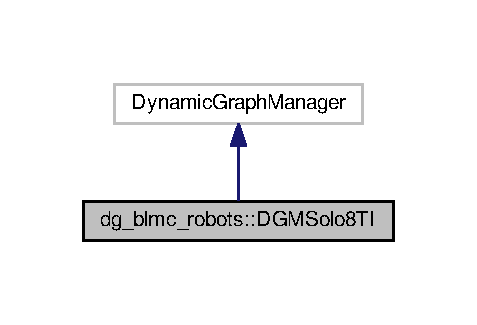
\includegraphics[width=229pt]{classdg__blmc__robots_1_1DGMSolo8TI__inherit__graph}
\end{center}
\end{figure}


Collaboration diagram for dg\+\_\+blmc\+\_\+robots\+:\+:D\+G\+M\+Solo8\+TI\+:
\nopagebreak
\begin{figure}[H]
\begin{center}
\leavevmode
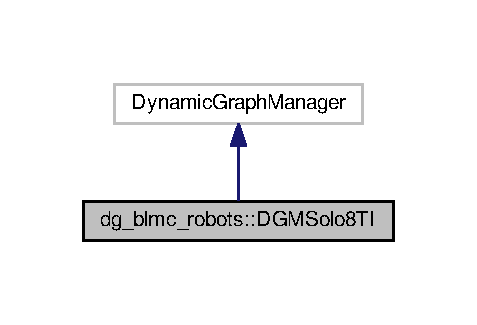
\includegraphics[width=229pt]{classdg__blmc__robots_1_1DGMSolo8TI__coll__graph}
\end{center}
\end{figure}
\subsection*{Public Member Functions}
\begin{DoxyCompactItemize}
\item 
\hyperlink{classdg__blmc__robots_1_1DGMSolo8TI_abee90d8f11708199fca29849b559cc81}{D\+G\+M\+Solo8\+TI} ()\hypertarget{classdg__blmc__robots_1_1DGMSolo8TI_abee90d8f11708199fca29849b559cc81}{}\label{classdg__blmc__robots_1_1DGMSolo8TI_abee90d8f11708199fca29849b559cc81}

\begin{DoxyCompactList}\small\item\em Demo\+Single\+Motor is the constructor. \end{DoxyCompactList}\item 
\hyperlink{classdg__blmc__robots_1_1DGMSolo8TI_adc55a8663b9682a54c50dea30ef66eaf}{$\sim$\+D\+G\+M\+Solo8\+TI} ()\hypertarget{classdg__blmc__robots_1_1DGMSolo8TI_adc55a8663b9682a54c50dea30ef66eaf}{}\label{classdg__blmc__robots_1_1DGMSolo8TI_adc55a8663b9682a54c50dea30ef66eaf}

\begin{DoxyCompactList}\small\item\em $\sim$\+Demo\+Single\+Motor is the destructor. \end{DoxyCompactList}\item 
void \hyperlink{classdg__blmc__robots_1_1DGMSolo8TI_a2a21728cb1b63fa63242514d09c2e7bf}{initialize\+\_\+hardware\+\_\+communication\+\_\+process} ()
\begin{DoxyCompactList}\small\item\em initialize\+\_\+hardware\+\_\+communication\+\_\+process is the function that initialize the hardware. \end{DoxyCompactList}\item 
void \hyperlink{classdg__blmc__robots_1_1DGMSolo8TI_afd126d69bc1d226c2666a4653e306b46}{get\+\_\+sensors\+\_\+to\+\_\+map} (dynamic\+\_\+graph\+::\+Vector\+D\+G\+Map \&map)
\begin{DoxyCompactList}\small\item\em get\+\_\+sensors\+\_\+to\+\_\+map acquieres the sensors data and feed it to the input/output map \end{DoxyCompactList}\item 
void \hyperlink{classdg__blmc__robots_1_1DGMSolo8TI_aef367ff385590dce6ca8fd4d8b10e813}{set\+\_\+motor\+\_\+controls\+\_\+from\+\_\+map} (const dynamic\+\_\+graph\+::\+Vector\+D\+G\+Map \&map)
\begin{DoxyCompactList}\small\item\em set\+\_\+motor\+\_\+controls\+\_\+from\+\_\+map reads the input map that contains the controls and send these controls to the hardware. \end{DoxyCompactList}\item 
bool \hyperlink{classdg__blmc__robots_1_1DGMSolo8TI_ab862135f110f2b497931892f6abbb879}{calibrate\+\_\+joint\+\_\+position\+\_\+callback} (dg\+\_\+blmc\+\_\+robots\+::\+Joint\+Calibration\+::\+Request \&req, dg\+\_\+blmc\+\_\+robots\+::\+Joint\+Calibration\+::\+Response \&res)
\begin{DoxyCompactList}\small\item\em Handle the calibrate\+\_\+joint callback. \end{DoxyCompactList}\end{DoxyCompactItemize}
\subsection*{Private Member Functions}
\begin{DoxyCompactItemize}
\item 
void \hyperlink{classdg__blmc__robots_1_1DGMSolo8TI_a9b4b07438fdce74f3875576ad8b38b9b}{calibrate\+\_\+joint\+\_\+position} (const blmc\+\_\+robots\+::\+Vector8d \&zero\+\_\+to\+\_\+index\+\_\+angle)
\begin{DoxyCompactList}\small\item\em Calibrate the robot joint position. \end{DoxyCompactList}\end{DoxyCompactItemize}
\subsection*{Private Attributes}
\begin{DoxyCompactItemize}
\item 
blmc\+\_\+robots\+::\+Solo8\+TI \hyperlink{classdg__blmc__robots_1_1DGMSolo8TI_ae1fd04476b371df57db40d6a97783731}{solo\+\_\+}
\begin{DoxyCompactList}\small\item\em Entries for the real hardware. \end{DoxyCompactList}\item 
blmc\+\_\+robots\+::\+Vector8d \hyperlink{classdg__blmc__robots_1_1DGMSolo8TI_accfae6534d5201f28278eeba0febb22e}{ctrl\+\_\+joint\+\_\+torques\+\_\+}
\begin{DoxyCompactList}\small\item\em ctrl\+\_\+joint\+\_\+torques\+\_\+ the joint torques to be sent. \end{DoxyCompactList}\item 
bool \hyperlink{classdg__blmc__robots_1_1DGMSolo8TI_a2f99efb27e8260c0f900a96e67e810db}{was\+\_\+in\+\_\+safety\+\_\+mode\+\_\+}\hypertarget{classdg__blmc__robots_1_1DGMSolo8TI_a2f99efb27e8260c0f900a96e67e810db}{}\label{classdg__blmc__robots_1_1DGMSolo8TI_a2f99efb27e8260c0f900a96e67e810db}

\begin{DoxyCompactList}\small\item\em Check if we entered once in the safety mode and stay there if so. \end{DoxyCompactList}\item 
blmc\+\_\+robots\+::\+Vector8d \hyperlink{classdg__blmc__robots_1_1DGMSolo8TI_a05609f544243050ecac91ec55c9d7066}{zero\+\_\+to\+\_\+index\+\_\+angle\+\_\+from\+\_\+file\+\_\+}
\begin{DoxyCompactList}\small\item\em These are the calibration value extracted from the paramters. \end{DoxyCompactList}\end{DoxyCompactItemize}


\subsection{Member Function Documentation}
\index{dg\+\_\+blmc\+\_\+robots\+::\+D\+G\+M\+Solo8\+TI@{dg\+\_\+blmc\+\_\+robots\+::\+D\+G\+M\+Solo8\+TI}!calibrate\+\_\+joint\+\_\+position@{calibrate\+\_\+joint\+\_\+position}}
\index{calibrate\+\_\+joint\+\_\+position@{calibrate\+\_\+joint\+\_\+position}!dg\+\_\+blmc\+\_\+robots\+::\+D\+G\+M\+Solo8\+TI@{dg\+\_\+blmc\+\_\+robots\+::\+D\+G\+M\+Solo8\+TI}}
\subsubsection[{\texorpdfstring{calibrate\+\_\+joint\+\_\+position(const blmc\+\_\+robots\+::\+Vector8d \&zero\+\_\+to\+\_\+index\+\_\+angle)}{calibrate_joint_position(const blmc_robots::Vector8d &zero_to_index_angle)}}]{\setlength{\rightskip}{0pt plus 5cm}void dg\+\_\+blmc\+\_\+robots\+::\+D\+G\+M\+Solo8\+T\+I\+::calibrate\+\_\+joint\+\_\+position (
\begin{DoxyParamCaption}
\item[{const blmc\+\_\+robots\+::\+Vector8d \&}]{zero\+\_\+to\+\_\+index\+\_\+angle}
\end{DoxyParamCaption}
)\hspace{0.3cm}{\ttfamily [private]}}\hypertarget{classdg__blmc__robots_1_1DGMSolo8TI_a9b4b07438fdce74f3875576ad8b38b9b}{}\label{classdg__blmc__robots_1_1DGMSolo8TI_a9b4b07438fdce74f3875576ad8b38b9b}


Calibrate the robot joint position. 


\begin{DoxyParams}{Parameters}
{\em zero\+\_\+to\+\_\+index\+\_\+angle} & is the angle between the theoretical zero and the next positive angle. \\
\hline
\end{DoxyParams}
\index{dg\+\_\+blmc\+\_\+robots\+::\+D\+G\+M\+Solo8\+TI@{dg\+\_\+blmc\+\_\+robots\+::\+D\+G\+M\+Solo8\+TI}!calibrate\+\_\+joint\+\_\+position\+\_\+callback@{calibrate\+\_\+joint\+\_\+position\+\_\+callback}}
\index{calibrate\+\_\+joint\+\_\+position\+\_\+callback@{calibrate\+\_\+joint\+\_\+position\+\_\+callback}!dg\+\_\+blmc\+\_\+robots\+::\+D\+G\+M\+Solo8\+TI@{dg\+\_\+blmc\+\_\+robots\+::\+D\+G\+M\+Solo8\+TI}}
\subsubsection[{\texorpdfstring{calibrate\+\_\+joint\+\_\+position\+\_\+callback(dg\+\_\+blmc\+\_\+robots\+::\+Joint\+Calibration\+::\+Request \&req, dg\+\_\+blmc\+\_\+robots\+::\+Joint\+Calibration\+::\+Response \&res)}{calibrate_joint_position_callback(dg_blmc_robots::JointCalibration::Request &req, dg_blmc_robots::JointCalibration::Response &res)}}]{\setlength{\rightskip}{0pt plus 5cm}bool dg\+\_\+blmc\+\_\+robots\+::\+D\+G\+M\+Solo8\+T\+I\+::calibrate\+\_\+joint\+\_\+position\+\_\+callback (
\begin{DoxyParamCaption}
\item[{dg\+\_\+blmc\+\_\+robots\+::\+Joint\+Calibration\+::\+Request \&}]{req, }
\item[{dg\+\_\+blmc\+\_\+robots\+::\+Joint\+Calibration\+::\+Response \&}]{res}
\end{DoxyParamCaption}
)}\hypertarget{classdg__blmc__robots_1_1DGMSolo8TI_ab862135f110f2b497931892f6abbb879}{}\label{classdg__blmc__robots_1_1DGMSolo8TI_ab862135f110f2b497931892f6abbb879}


Handle the calibrate\+\_\+joint callback. 


\begin{DoxyParams}{Parameters}
{\em req} & R\+OS request. \\
\hline
{\em res} & R\+OS response. \\
\hline
\end{DoxyParams}
\begin{DoxyReturn}{Returns}
True if calibration was successful, false otherwise. 
\end{DoxyReturn}
\index{dg\+\_\+blmc\+\_\+robots\+::\+D\+G\+M\+Solo8\+TI@{dg\+\_\+blmc\+\_\+robots\+::\+D\+G\+M\+Solo8\+TI}!get\+\_\+sensors\+\_\+to\+\_\+map@{get\+\_\+sensors\+\_\+to\+\_\+map}}
\index{get\+\_\+sensors\+\_\+to\+\_\+map@{get\+\_\+sensors\+\_\+to\+\_\+map}!dg\+\_\+blmc\+\_\+robots\+::\+D\+G\+M\+Solo8\+TI@{dg\+\_\+blmc\+\_\+robots\+::\+D\+G\+M\+Solo8\+TI}}
\subsubsection[{\texorpdfstring{get\+\_\+sensors\+\_\+to\+\_\+map(dynamic\+\_\+graph\+::\+Vector\+D\+G\+Map \&map)}{get_sensors_to_map(dynamic_graph::VectorDGMap &map)}}]{\setlength{\rightskip}{0pt plus 5cm}void dg\+\_\+blmc\+\_\+robots\+::\+D\+G\+M\+Solo8\+T\+I\+::get\+\_\+sensors\+\_\+to\+\_\+map (
\begin{DoxyParamCaption}
\item[{dynamic\+\_\+graph\+::\+Vector\+D\+G\+Map \&}]{map}
\end{DoxyParamCaption}
)}\hypertarget{classdg__blmc__robots_1_1DGMSolo8TI_afd126d69bc1d226c2666a4653e306b46}{}\label{classdg__blmc__robots_1_1DGMSolo8TI_afd126d69bc1d226c2666a4653e306b46}


get\+\_\+sensors\+\_\+to\+\_\+map acquieres the sensors data and feed it to the input/output map 


\begin{DoxyParams}[1]{Parameters}
\mbox{\tt in}  & {\em } & \\
\hline
\end{DoxyParams}
Joint data

Additional data

Robot status\index{dg\+\_\+blmc\+\_\+robots\+::\+D\+G\+M\+Solo8\+TI@{dg\+\_\+blmc\+\_\+robots\+::\+D\+G\+M\+Solo8\+TI}!initialize\+\_\+hardware\+\_\+communication\+\_\+process@{initialize\+\_\+hardware\+\_\+communication\+\_\+process}}
\index{initialize\+\_\+hardware\+\_\+communication\+\_\+process@{initialize\+\_\+hardware\+\_\+communication\+\_\+process}!dg\+\_\+blmc\+\_\+robots\+::\+D\+G\+M\+Solo8\+TI@{dg\+\_\+blmc\+\_\+robots\+::\+D\+G\+M\+Solo8\+TI}}
\subsubsection[{\texorpdfstring{initialize\+\_\+hardware\+\_\+communication\+\_\+process()}{initialize_hardware_communication_process()}}]{\setlength{\rightskip}{0pt plus 5cm}void dg\+\_\+blmc\+\_\+robots\+::\+D\+G\+M\+Solo8\+T\+I\+::initialize\+\_\+hardware\+\_\+communication\+\_\+process (
\begin{DoxyParamCaption}
{}
\end{DoxyParamCaption}
)}\hypertarget{classdg__blmc__robots_1_1DGMSolo8TI_a2a21728cb1b63fa63242514d09c2e7bf}{}\label{classdg__blmc__robots_1_1DGMSolo8TI_a2a21728cb1b63fa63242514d09c2e7bf}


initialize\+\_\+hardware\+\_\+communication\+\_\+process is the function that initialize the hardware. 

Load the calibration parameters

initialize the user commands \index{dg\+\_\+blmc\+\_\+robots\+::\+D\+G\+M\+Solo8\+TI@{dg\+\_\+blmc\+\_\+robots\+::\+D\+G\+M\+Solo8\+TI}!set\+\_\+motor\+\_\+controls\+\_\+from\+\_\+map@{set\+\_\+motor\+\_\+controls\+\_\+from\+\_\+map}}
\index{set\+\_\+motor\+\_\+controls\+\_\+from\+\_\+map@{set\+\_\+motor\+\_\+controls\+\_\+from\+\_\+map}!dg\+\_\+blmc\+\_\+robots\+::\+D\+G\+M\+Solo8\+TI@{dg\+\_\+blmc\+\_\+robots\+::\+D\+G\+M\+Solo8\+TI}}
\subsubsection[{\texorpdfstring{set\+\_\+motor\+\_\+controls\+\_\+from\+\_\+map(const dynamic\+\_\+graph\+::\+Vector\+D\+G\+Map \&map)}{set_motor_controls_from_map(const dynamic_graph::VectorDGMap &map)}}]{\setlength{\rightskip}{0pt plus 5cm}void dg\+\_\+blmc\+\_\+robots\+::\+D\+G\+M\+Solo8\+T\+I\+::set\+\_\+motor\+\_\+controls\+\_\+from\+\_\+map (
\begin{DoxyParamCaption}
\item[{const dynamic\+\_\+graph\+::\+Vector\+D\+G\+Map \&}]{map}
\end{DoxyParamCaption}
)}\hypertarget{classdg__blmc__robots_1_1DGMSolo8TI_aef367ff385590dce6ca8fd4d8b10e813}{}\label{classdg__blmc__robots_1_1DGMSolo8TI_aef367ff385590dce6ca8fd4d8b10e813}


set\+\_\+motor\+\_\+controls\+\_\+from\+\_\+map reads the input map that contains the controls and send these controls to the hardware. 


\begin{DoxyParams}{Parameters}
{\em map} & \\
\hline
\end{DoxyParams}


\subsection{Member Data Documentation}
\index{dg\+\_\+blmc\+\_\+robots\+::\+D\+G\+M\+Solo8\+TI@{dg\+\_\+blmc\+\_\+robots\+::\+D\+G\+M\+Solo8\+TI}!ctrl\+\_\+joint\+\_\+torques\+\_\+@{ctrl\+\_\+joint\+\_\+torques\+\_\+}}
\index{ctrl\+\_\+joint\+\_\+torques\+\_\+@{ctrl\+\_\+joint\+\_\+torques\+\_\+}!dg\+\_\+blmc\+\_\+robots\+::\+D\+G\+M\+Solo8\+TI@{dg\+\_\+blmc\+\_\+robots\+::\+D\+G\+M\+Solo8\+TI}}
\subsubsection[{\texorpdfstring{ctrl\+\_\+joint\+\_\+torques\+\_\+}{ctrl_joint_torques_}}]{\setlength{\rightskip}{0pt plus 5cm}blmc\+\_\+robots\+::\+Vector8d dg\+\_\+blmc\+\_\+robots\+::\+D\+G\+M\+Solo8\+T\+I\+::ctrl\+\_\+joint\+\_\+torques\+\_\+\hspace{0.3cm}{\ttfamily [private]}}\hypertarget{classdg__blmc__robots_1_1DGMSolo8TI_accfae6534d5201f28278eeba0febb22e}{}\label{classdg__blmc__robots_1_1DGMSolo8TI_accfae6534d5201f28278eeba0febb22e}


ctrl\+\_\+joint\+\_\+torques\+\_\+ the joint torques to be sent. 

Used in this class to perform a local copy of the control. This is need in order to send this copy to the blmc\+\_\+robots\+::\+Solo class \index{dg\+\_\+blmc\+\_\+robots\+::\+D\+G\+M\+Solo8\+TI@{dg\+\_\+blmc\+\_\+robots\+::\+D\+G\+M\+Solo8\+TI}!solo\+\_\+@{solo\+\_\+}}
\index{solo\+\_\+@{solo\+\_\+}!dg\+\_\+blmc\+\_\+robots\+::\+D\+G\+M\+Solo8\+TI@{dg\+\_\+blmc\+\_\+robots\+::\+D\+G\+M\+Solo8\+TI}}
\subsubsection[{\texorpdfstring{solo\+\_\+}{solo_}}]{\setlength{\rightskip}{0pt plus 5cm}blmc\+\_\+robots\+::\+Solo8\+TI dg\+\_\+blmc\+\_\+robots\+::\+D\+G\+M\+Solo8\+T\+I\+::solo\+\_\+\hspace{0.3cm}{\ttfamily [private]}}\hypertarget{classdg__blmc__robots_1_1DGMSolo8TI_ae1fd04476b371df57db40d6a97783731}{}\label{classdg__blmc__robots_1_1DGMSolo8TI_ae1fd04476b371df57db40d6a97783731}


Entries for the real hardware. 

test\+\_\+bench\+\_\+ the real test bench hardware drivers. \index{dg\+\_\+blmc\+\_\+robots\+::\+D\+G\+M\+Solo8\+TI@{dg\+\_\+blmc\+\_\+robots\+::\+D\+G\+M\+Solo8\+TI}!zero\+\_\+to\+\_\+index\+\_\+angle\+\_\+from\+\_\+file\+\_\+@{zero\+\_\+to\+\_\+index\+\_\+angle\+\_\+from\+\_\+file\+\_\+}}
\index{zero\+\_\+to\+\_\+index\+\_\+angle\+\_\+from\+\_\+file\+\_\+@{zero\+\_\+to\+\_\+index\+\_\+angle\+\_\+from\+\_\+file\+\_\+}!dg\+\_\+blmc\+\_\+robots\+::\+D\+G\+M\+Solo8\+TI@{dg\+\_\+blmc\+\_\+robots\+::\+D\+G\+M\+Solo8\+TI}}
\subsubsection[{\texorpdfstring{zero\+\_\+to\+\_\+index\+\_\+angle\+\_\+from\+\_\+file\+\_\+}{zero_to_index_angle_from_file_}}]{\setlength{\rightskip}{0pt plus 5cm}blmc\+\_\+robots\+::\+Vector8d dg\+\_\+blmc\+\_\+robots\+::\+D\+G\+M\+Solo8\+T\+I\+::zero\+\_\+to\+\_\+index\+\_\+angle\+\_\+from\+\_\+file\+\_\+\hspace{0.3cm}{\ttfamily [private]}}\hypertarget{classdg__blmc__robots_1_1DGMSolo8TI_a05609f544243050ecac91ec55c9d7066}{}\label{classdg__blmc__robots_1_1DGMSolo8TI_a05609f544243050ecac91ec55c9d7066}


These are the calibration value extracted from the paramters. 

They represent the distance between the theorical zero joint angle and the next jont index. 

The documentation for this class was generated from the following files\+:\begin{DoxyCompactItemize}
\item 
include/dg\+\_\+blmc\+\_\+robots/dgm\+\_\+solo8ti.\+hpp\item 
src/dgm\+\_\+solo8ti.\+cpp\end{DoxyCompactItemize}

\hypertarget{classdg__blmc__robots_1_1DGMStuggihop}{}\section{dg\+\_\+blmc\+\_\+robots\+:\+:D\+G\+M\+Stuggihop Class Reference}
\label{classdg__blmc__robots_1_1DGMStuggihop}\index{dg\+\_\+blmc\+\_\+robots\+::\+D\+G\+M\+Stuggihop@{dg\+\_\+blmc\+\_\+robots\+::\+D\+G\+M\+Stuggihop}}


Inheritance diagram for dg\+\_\+blmc\+\_\+robots\+:\+:D\+G\+M\+Stuggihop\+:
\nopagebreak
\begin{figure}[H]
\begin{center}
\leavevmode
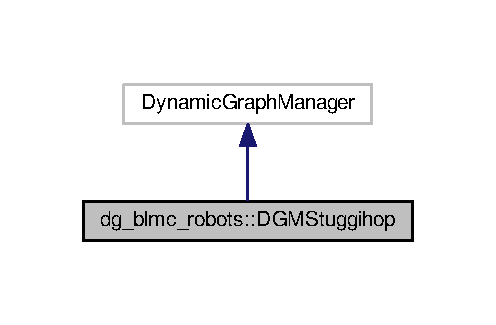
\includegraphics[width=238pt]{classdg__blmc__robots_1_1DGMStuggihop__inherit__graph}
\end{center}
\end{figure}


Collaboration diagram for dg\+\_\+blmc\+\_\+robots\+:\+:D\+G\+M\+Stuggihop\+:
\nopagebreak
\begin{figure}[H]
\begin{center}
\leavevmode
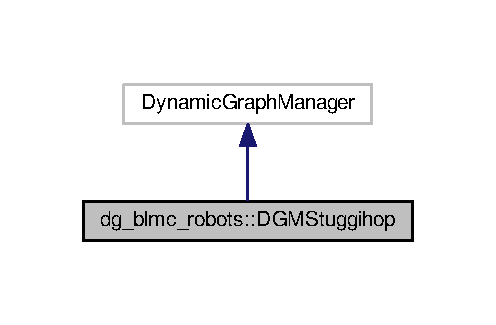
\includegraphics[width=238pt]{classdg__blmc__robots_1_1DGMStuggihop__coll__graph}
\end{center}
\end{figure}
\subsection*{Public Member Functions}
\begin{DoxyCompactItemize}
\item 
\hyperlink{classdg__blmc__robots_1_1DGMStuggihop_a00d09c7496216833d0bbf9528dc91bf1}{D\+G\+M\+Stuggihop} ()\hypertarget{classdg__blmc__robots_1_1DGMStuggihop_a00d09c7496216833d0bbf9528dc91bf1}{}\label{classdg__blmc__robots_1_1DGMStuggihop_a00d09c7496216833d0bbf9528dc91bf1}

\begin{DoxyCompactList}\small\item\em \hyperlink{classdg__blmc__robots_1_1DGMStuggihop}{D\+G\+M\+Stuggihop} is the constructor. \end{DoxyCompactList}\item 
\hyperlink{classdg__blmc__robots_1_1DGMStuggihop_abf9d5debbb1dfd891f721afaf37aaa7b}{$\sim$\+D\+G\+M\+Stuggihop} ()\hypertarget{classdg__blmc__robots_1_1DGMStuggihop_abf9d5debbb1dfd891f721afaf37aaa7b}{}\label{classdg__blmc__robots_1_1DGMStuggihop_abf9d5debbb1dfd891f721afaf37aaa7b}

\begin{DoxyCompactList}\small\item\em $\sim$\+D\+G\+M\+Stuggihop is the destructor. \end{DoxyCompactList}\item 
void \hyperlink{classdg__blmc__robots_1_1DGMStuggihop_ab19867edf16d958dbdc053f719b8c328}{initialize\+\_\+hardware\+\_\+communication\+\_\+process} ()\hypertarget{classdg__blmc__robots_1_1DGMStuggihop_ab19867edf16d958dbdc053f719b8c328}{}\label{classdg__blmc__robots_1_1DGMStuggihop_ab19867edf16d958dbdc053f719b8c328}

\begin{DoxyCompactList}\small\item\em initialize\+\_\+hardware\+\_\+communication\+\_\+process is the function that initialize the hardware. \end{DoxyCompactList}\item 
void \hyperlink{classdg__blmc__robots_1_1DGMStuggihop_a0a54f99691e07866000b28c028947957}{get\+\_\+sensors\+\_\+to\+\_\+map} (dynamic\+\_\+graph\+::\+Vector\+D\+G\+Map \&map)
\begin{DoxyCompactList}\small\item\em get\+\_\+sensors\+\_\+to\+\_\+map acquires the sensors data and feeds it to the input/output map \end{DoxyCompactList}\item 
void \hyperlink{classdg__blmc__robots_1_1DGMStuggihop_a17b70b0c18502cc60461b94f0ca2148b}{set\+\_\+motor\+\_\+controls\+\_\+from\+\_\+map} (const dynamic\+\_\+graph\+::\+Vector\+D\+G\+Map \&map)
\begin{DoxyCompactList}\small\item\em set\+\_\+motor\+\_\+controls\+\_\+from\+\_\+map reads the input map that contains the controls and send these controls to the hardware. \end{DoxyCompactList}\item 
virtual bool \hyperlink{classdg__blmc__robots_1_1DGMStuggihop_a5834264acad3d97e9fb5cdf9c404b875}{is\+\_\+in\+\_\+safety\+\_\+mode} ()\hypertarget{classdg__blmc__robots_1_1DGMStuggihop_a5834264acad3d97e9fb5cdf9c404b875}{}\label{classdg__blmc__robots_1_1DGMStuggihop_a5834264acad3d97e9fb5cdf9c404b875}

\begin{DoxyCompactList}\small\item\em is\+\_\+in\+\_\+safety\+\_\+mode Implement custom safe-\/mode detection. \end{DoxyCompactList}\end{DoxyCompactItemize}
\subsection*{Private Attributes}
\begin{DoxyCompactItemize}
\item 
blmc\+\_\+robots\+::\+Stuggihop \hyperlink{classdg__blmc__robots_1_1DGMStuggihop_a70126fb0319274141ab4a6193e7c7121}{stuggihop\+\_\+}
\begin{DoxyCompactList}\small\item\em Entries for the real hardware. \end{DoxyCompactList}\item 
Eigen\+::\+Vector2d \hyperlink{classdg__blmc__robots_1_1DGMStuggihop_afb2035bb08deca1f64ec1284dcf8dfff}{ctrl\+\_\+joint\+\_\+torques\+\_\+}\hypertarget{classdg__blmc__robots_1_1DGMStuggihop_afb2035bb08deca1f64ec1284dcf8dfff}{}\label{classdg__blmc__robots_1_1DGMStuggihop_afb2035bb08deca1f64ec1284dcf8dfff}

\begin{DoxyCompactList}\small\item\em ctrl\+\_\+joint\+\_\+torques\+\_\+ the joint torques to be sent \end{DoxyCompactList}\item 
bool \hyperlink{classdg__blmc__robots_1_1DGMStuggihop_ac2491e5f7993fc8d1bcbc7af4da69f86}{was\+\_\+in\+\_\+safety\+\_\+mode\+\_\+}\hypertarget{classdg__blmc__robots_1_1DGMStuggihop_ac2491e5f7993fc8d1bcbc7af4da69f86}{}\label{classdg__blmc__robots_1_1DGMStuggihop_ac2491e5f7993fc8d1bcbc7af4da69f86}

\begin{DoxyCompactList}\small\item\em was\+\_\+in\+\_\+safety\+\_\+mode\+\_\+ Toggle to keep in safety mode once it was entered. \end{DoxyCompactList}\end{DoxyCompactItemize}


\subsection{Member Function Documentation}
\index{dg\+\_\+blmc\+\_\+robots\+::\+D\+G\+M\+Stuggihop@{dg\+\_\+blmc\+\_\+robots\+::\+D\+G\+M\+Stuggihop}!get\+\_\+sensors\+\_\+to\+\_\+map@{get\+\_\+sensors\+\_\+to\+\_\+map}}
\index{get\+\_\+sensors\+\_\+to\+\_\+map@{get\+\_\+sensors\+\_\+to\+\_\+map}!dg\+\_\+blmc\+\_\+robots\+::\+D\+G\+M\+Stuggihop@{dg\+\_\+blmc\+\_\+robots\+::\+D\+G\+M\+Stuggihop}}
\subsubsection[{\texorpdfstring{get\+\_\+sensors\+\_\+to\+\_\+map(dynamic\+\_\+graph\+::\+Vector\+D\+G\+Map \&map)}{get_sensors_to_map(dynamic_graph::VectorDGMap &map)}}]{\setlength{\rightskip}{0pt plus 5cm}void dg\+\_\+blmc\+\_\+robots\+::\+D\+G\+M\+Stuggihop\+::get\+\_\+sensors\+\_\+to\+\_\+map (
\begin{DoxyParamCaption}
\item[{dynamic\+\_\+graph\+::\+Vector\+D\+G\+Map \&}]{map}
\end{DoxyParamCaption}
)}\hypertarget{classdg__blmc__robots_1_1DGMStuggihop_a0a54f99691e07866000b28c028947957}{}\label{classdg__blmc__robots_1_1DGMStuggihop_a0a54f99691e07866000b28c028947957}


get\+\_\+sensors\+\_\+to\+\_\+map acquires the sensors data and feeds it to the input/output map 


\begin{DoxyParams}[1]{Parameters}
\mbox{\tt in}  & {\em } & \\
\hline
\end{DoxyParams}
Joint data

Additional data

Motor data T\+O\+DO\+: erroneous?

Joint data

Additional data\index{dg\+\_\+blmc\+\_\+robots\+::\+D\+G\+M\+Stuggihop@{dg\+\_\+blmc\+\_\+robots\+::\+D\+G\+M\+Stuggihop}!set\+\_\+motor\+\_\+controls\+\_\+from\+\_\+map@{set\+\_\+motor\+\_\+controls\+\_\+from\+\_\+map}}
\index{set\+\_\+motor\+\_\+controls\+\_\+from\+\_\+map@{set\+\_\+motor\+\_\+controls\+\_\+from\+\_\+map}!dg\+\_\+blmc\+\_\+robots\+::\+D\+G\+M\+Stuggihop@{dg\+\_\+blmc\+\_\+robots\+::\+D\+G\+M\+Stuggihop}}
\subsubsection[{\texorpdfstring{set\+\_\+motor\+\_\+controls\+\_\+from\+\_\+map(const dynamic\+\_\+graph\+::\+Vector\+D\+G\+Map \&map)}{set_motor_controls_from_map(const dynamic_graph::VectorDGMap &map)}}]{\setlength{\rightskip}{0pt plus 5cm}void dg\+\_\+blmc\+\_\+robots\+::\+D\+G\+M\+Stuggihop\+::set\+\_\+motor\+\_\+controls\+\_\+from\+\_\+map (
\begin{DoxyParamCaption}
\item[{const dynamic\+\_\+graph\+::\+Vector\+D\+G\+Map \&}]{map}
\end{DoxyParamCaption}
)}\hypertarget{classdg__blmc__robots_1_1DGMStuggihop_a17b70b0c18502cc60461b94f0ca2148b}{}\label{classdg__blmc__robots_1_1DGMStuggihop_a17b70b0c18502cc60461b94f0ca2148b}


set\+\_\+motor\+\_\+controls\+\_\+from\+\_\+map reads the input map that contains the controls and send these controls to the hardware. 


\begin{DoxyParams}{Parameters}
{\em map} & \\
\hline
\end{DoxyParams}


\subsection{Member Data Documentation}
\index{dg\+\_\+blmc\+\_\+robots\+::\+D\+G\+M\+Stuggihop@{dg\+\_\+blmc\+\_\+robots\+::\+D\+G\+M\+Stuggihop}!stuggihop\+\_\+@{stuggihop\+\_\+}}
\index{stuggihop\+\_\+@{stuggihop\+\_\+}!dg\+\_\+blmc\+\_\+robots\+::\+D\+G\+M\+Stuggihop@{dg\+\_\+blmc\+\_\+robots\+::\+D\+G\+M\+Stuggihop}}
\subsubsection[{\texorpdfstring{stuggihop\+\_\+}{stuggihop_}}]{\setlength{\rightskip}{0pt plus 5cm}blmc\+\_\+robots\+::\+Stuggihop dg\+\_\+blmc\+\_\+robots\+::\+D\+G\+M\+Stuggihop\+::stuggihop\+\_\+\hspace{0.3cm}{\ttfamily [private]}}\hypertarget{classdg__blmc__robots_1_1DGMStuggihop_a70126fb0319274141ab4a6193e7c7121}{}\label{classdg__blmc__robots_1_1DGMStuggihop_a70126fb0319274141ab4a6193e7c7121}


Entries for the real hardware. 

test\+\_\+bench\+\_\+ the real test bench hardware drivers. 

The documentation for this class was generated from the following files\+:\begin{DoxyCompactItemize}
\item 
include/dg\+\_\+blmc\+\_\+robots/\hyperlink{dgm__stuggihop_8hpp}{dgm\+\_\+stuggihop.\+hpp}\item 
src/\hyperlink{dgm__stuggihop_8cpp}{dgm\+\_\+stuggihop.\+cpp}\end{DoxyCompactItemize}

\hypertarget{classdg__blmc__robots_1_1DGMTeststand}{}\section{dg\+\_\+blmc\+\_\+robots\+:\+:D\+G\+M\+Teststand Class Reference}
\label{classdg__blmc__robots_1_1DGMTeststand}\index{dg\+\_\+blmc\+\_\+robots\+::\+D\+G\+M\+Teststand@{dg\+\_\+blmc\+\_\+robots\+::\+D\+G\+M\+Teststand}}


Inheritance diagram for dg\+\_\+blmc\+\_\+robots\+:\+:D\+G\+M\+Teststand\+:
\nopagebreak
\begin{figure}[H]
\begin{center}
\leavevmode
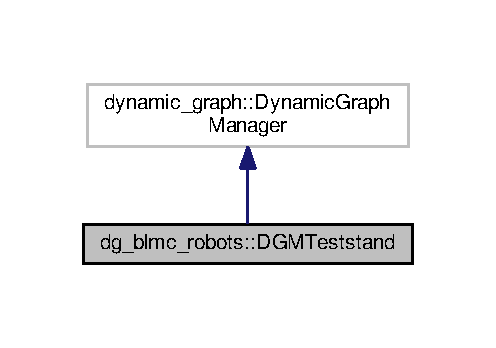
\includegraphics[width=238pt]{classdg__blmc__robots_1_1DGMTeststand__inherit__graph}
\end{center}
\end{figure}


Collaboration diagram for dg\+\_\+blmc\+\_\+robots\+:\+:D\+G\+M\+Teststand\+:
\nopagebreak
\begin{figure}[H]
\begin{center}
\leavevmode
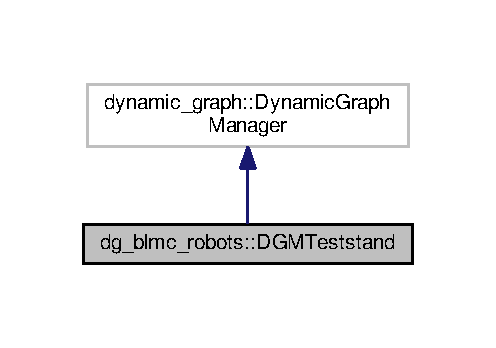
\includegraphics[width=238pt]{classdg__blmc__robots_1_1DGMTeststand__coll__graph}
\end{center}
\end{figure}
\subsection*{Public Member Functions}
\begin{DoxyCompactItemize}
\item 
\hyperlink{classdg__blmc__robots_1_1DGMTeststand_ae6b6e00fbd3460f7083977ae9befb6fd}{D\+G\+M\+Teststand} ()\hypertarget{classdg__blmc__robots_1_1DGMTeststand_ae6b6e00fbd3460f7083977ae9befb6fd}{}\label{classdg__blmc__robots_1_1DGMTeststand_ae6b6e00fbd3460f7083977ae9befb6fd}

\begin{DoxyCompactList}\small\item\em \hyperlink{classdg__blmc__robots_1_1DGMTeststand}{D\+G\+M\+Teststand} is the constructor. \end{DoxyCompactList}\item 
\hyperlink{classdg__blmc__robots_1_1DGMTeststand_a8699f157b5a05c92a5de2b2c80ba70af}{$\sim$\+D\+G\+M\+Teststand} ()\hypertarget{classdg__blmc__robots_1_1DGMTeststand_a8699f157b5a05c92a5de2b2c80ba70af}{}\label{classdg__blmc__robots_1_1DGMTeststand_a8699f157b5a05c92a5de2b2c80ba70af}

\begin{DoxyCompactList}\small\item\em $\sim$\+D\+G\+M\+Teststand is the destructor. \end{DoxyCompactList}\item 
void \hyperlink{classdg__blmc__robots_1_1DGMTeststand_a8495e1f1eb764ff3118d0e8dc60bc686}{initialize\+\_\+hardware\+\_\+communication\+\_\+process} ()
\begin{DoxyCompactList}\small\item\em initialize\+\_\+hardware\+\_\+communication\+\_\+process is the function that initialize the hardware. \end{DoxyCompactList}\item 
void \hyperlink{classdg__blmc__robots_1_1DGMTeststand_ac0f85de90afcf35c01930f3504c8ac0e}{get\+\_\+sensors\+\_\+to\+\_\+map} (dynamic\+\_\+graph\+::\+Vector\+D\+G\+Map \&map)
\begin{DoxyCompactList}\small\item\em get\+\_\+sensors\+\_\+to\+\_\+map acquires the sensors data and feeds it to the input/output map \end{DoxyCompactList}\item 
void \hyperlink{classdg__blmc__robots_1_1DGMTeststand_a8b0ec086e17a6aae248c5c05014ad8a5}{set\+\_\+motor\+\_\+controls\+\_\+from\+\_\+map} (const dynamic\+\_\+graph\+::\+Vector\+D\+G\+Map \&map)
\begin{DoxyCompactList}\small\item\em set\+\_\+motor\+\_\+controls\+\_\+from\+\_\+map reads the input map that contains the controls and send these controls to the hardware. \end{DoxyCompactList}\item 
virtual bool \hyperlink{classdg__blmc__robots_1_1DGMTeststand_a90fd2d9a7e579cbeb9daf2f0ba0d2a02}{is\+\_\+in\+\_\+safety\+\_\+mode} ()\hypertarget{classdg__blmc__robots_1_1DGMTeststand_a90fd2d9a7e579cbeb9daf2f0ba0d2a02}{}\label{classdg__blmc__robots_1_1DGMTeststand_a90fd2d9a7e579cbeb9daf2f0ba0d2a02}

\begin{DoxyCompactList}\small\item\em is\+\_\+in\+\_\+safety\+\_\+mode Implement custom safe-\/mode detection. \end{DoxyCompactList}\item 
bool \hyperlink{classdg__blmc__robots_1_1DGMTeststand_a133087f3899672101df62fbf95fac292}{calibrate\+\_\+joint\+\_\+position\+\_\+callback} (dg\+\_\+blmc\+\_\+robots\+::\+Joint\+Calibration\+::\+Request \&req, dg\+\_\+blmc\+\_\+robots\+::\+Joint\+Calibration\+::\+Response \&res)
\begin{DoxyCompactList}\small\item\em R\+OS callback. \end{DoxyCompactList}\end{DoxyCompactItemize}
\subsection*{Private Member Functions}
\begin{DoxyCompactItemize}
\item 
void \hyperlink{classdg__blmc__robots_1_1DGMTeststand_a0bce1340d617bfd6665cebef4d091ab1}{calibrate\+\_\+joint\+\_\+position} (const Eigen\+::\+Vector2d \&zero\+\_\+to\+\_\+index\+\_\+angle)
\begin{DoxyCompactList}\small\item\em Calibrate the robot joint position. \end{DoxyCompactList}\end{DoxyCompactItemize}
\subsection*{Private Attributes}
\begin{DoxyCompactItemize}
\item 
blmc\+\_\+robots\+::\+Teststand \hyperlink{classdg__blmc__robots_1_1DGMTeststand_a682499397e16186076999d8705e12c95}{teststand\+\_\+}
\begin{DoxyCompactList}\small\item\em Entries for the real hardware. \end{DoxyCompactList}\item 
Eigen\+::\+Vector2d \hyperlink{classdg__blmc__robots_1_1DGMTeststand_a7c5db196b671570171458720ea4341a8}{ctrl\+\_\+joint\+\_\+torques\+\_\+}\hypertarget{classdg__blmc__robots_1_1DGMTeststand_a7c5db196b671570171458720ea4341a8}{}\label{classdg__blmc__robots_1_1DGMTeststand_a7c5db196b671570171458720ea4341a8}

\begin{DoxyCompactList}\small\item\em ctrl\+\_\+joint\+\_\+torques\+\_\+ the joint torques to be sent \end{DoxyCompactList}\item 
Eigen\+::\+Vector2d \hyperlink{classdg__blmc__robots_1_1DGMTeststand_a788ef9391e891af10ab9b76f18139e5c}{zero\+\_\+to\+\_\+index\+\_\+angle\+\_\+from\+\_\+file\+\_\+}
\begin{DoxyCompactList}\small\item\em These are the calibration value extracted from the paramters. \end{DoxyCompactList}\item 
bool \hyperlink{classdg__blmc__robots_1_1DGMTeststand_a5821be382bfd2ec8b5bb668b2aacc2ea}{was\+\_\+in\+\_\+safety\+\_\+mode\+\_\+}\hypertarget{classdg__blmc__robots_1_1DGMTeststand_a5821be382bfd2ec8b5bb668b2aacc2ea}{}\label{classdg__blmc__robots_1_1DGMTeststand_a5821be382bfd2ec8b5bb668b2aacc2ea}

\begin{DoxyCompactList}\small\item\em was\+\_\+in\+\_\+safety\+\_\+mode\+\_\+ Toggle to keep in safety mode once it was entered. \end{DoxyCompactList}\end{DoxyCompactItemize}


\subsection{Member Function Documentation}
\index{dg\+\_\+blmc\+\_\+robots\+::\+D\+G\+M\+Teststand@{dg\+\_\+blmc\+\_\+robots\+::\+D\+G\+M\+Teststand}!calibrate\+\_\+joint\+\_\+position@{calibrate\+\_\+joint\+\_\+position}}
\index{calibrate\+\_\+joint\+\_\+position@{calibrate\+\_\+joint\+\_\+position}!dg\+\_\+blmc\+\_\+robots\+::\+D\+G\+M\+Teststand@{dg\+\_\+blmc\+\_\+robots\+::\+D\+G\+M\+Teststand}}
\subsubsection[{\texorpdfstring{calibrate\+\_\+joint\+\_\+position(const Eigen\+::\+Vector2d \&zero\+\_\+to\+\_\+index\+\_\+angle)}{calibrate_joint_position(const Eigen::Vector2d &zero_to_index_angle)}}]{\setlength{\rightskip}{0pt plus 5cm}void dg\+\_\+blmc\+\_\+robots\+::\+D\+G\+M\+Teststand\+::calibrate\+\_\+joint\+\_\+position (
\begin{DoxyParamCaption}
\item[{const Eigen\+::\+Vector2d \&}]{zero\+\_\+to\+\_\+index\+\_\+angle}
\end{DoxyParamCaption}
)\hspace{0.3cm}{\ttfamily [private]}}\hypertarget{classdg__blmc__robots_1_1DGMTeststand_a0bce1340d617bfd6665cebef4d091ab1}{}\label{classdg__blmc__robots_1_1DGMTeststand_a0bce1340d617bfd6665cebef4d091ab1}


Calibrate the robot joint position. 


\begin{DoxyParams}{Parameters}
{\em zero\+\_\+to\+\_\+index\+\_\+angle} & is the angle between the theoretical zero and the next positive angle. \\
\hline
\end{DoxyParams}
\index{dg\+\_\+blmc\+\_\+robots\+::\+D\+G\+M\+Teststand@{dg\+\_\+blmc\+\_\+robots\+::\+D\+G\+M\+Teststand}!calibrate\+\_\+joint\+\_\+position\+\_\+callback@{calibrate\+\_\+joint\+\_\+position\+\_\+callback}}
\index{calibrate\+\_\+joint\+\_\+position\+\_\+callback@{calibrate\+\_\+joint\+\_\+position\+\_\+callback}!dg\+\_\+blmc\+\_\+robots\+::\+D\+G\+M\+Teststand@{dg\+\_\+blmc\+\_\+robots\+::\+D\+G\+M\+Teststand}}
\subsubsection[{\texorpdfstring{calibrate\+\_\+joint\+\_\+position\+\_\+callback(dg\+\_\+blmc\+\_\+robots\+::\+Joint\+Calibration\+::\+Request \&req, dg\+\_\+blmc\+\_\+robots\+::\+Joint\+Calibration\+::\+Response \&res)}{calibrate_joint_position_callback(dg_blmc_robots::JointCalibration::Request &req, dg_blmc_robots::JointCalibration::Response &res)}}]{\setlength{\rightskip}{0pt plus 5cm}bool dg\+\_\+blmc\+\_\+robots\+::\+D\+G\+M\+Teststand\+::calibrate\+\_\+joint\+\_\+position\+\_\+callback (
\begin{DoxyParamCaption}
\item[{dg\+\_\+blmc\+\_\+robots\+::\+Joint\+Calibration\+::\+Request \&}]{req, }
\item[{dg\+\_\+blmc\+\_\+robots\+::\+Joint\+Calibration\+::\+Response \&}]{res}
\end{DoxyParamCaption}
)}\hypertarget{classdg__blmc__robots_1_1DGMTeststand_a133087f3899672101df62fbf95fac292}{}\label{classdg__blmc__robots_1_1DGMTeststand_a133087f3899672101df62fbf95fac292}


R\+OS callback. 


\begin{DoxyParams}{Parameters}
{\em req} & \\
\hline
{\em res} & \\
\hline
\end{DoxyParams}
\begin{DoxyReturn}{Returns}
true 

false 
\end{DoxyReturn}
\index{dg\+\_\+blmc\+\_\+robots\+::\+D\+G\+M\+Teststand@{dg\+\_\+blmc\+\_\+robots\+::\+D\+G\+M\+Teststand}!get\+\_\+sensors\+\_\+to\+\_\+map@{get\+\_\+sensors\+\_\+to\+\_\+map}}
\index{get\+\_\+sensors\+\_\+to\+\_\+map@{get\+\_\+sensors\+\_\+to\+\_\+map}!dg\+\_\+blmc\+\_\+robots\+::\+D\+G\+M\+Teststand@{dg\+\_\+blmc\+\_\+robots\+::\+D\+G\+M\+Teststand}}
\subsubsection[{\texorpdfstring{get\+\_\+sensors\+\_\+to\+\_\+map(dynamic\+\_\+graph\+::\+Vector\+D\+G\+Map \&map)}{get_sensors_to_map(dynamic_graph::VectorDGMap &map)}}]{\setlength{\rightskip}{0pt plus 5cm}void dg\+\_\+blmc\+\_\+robots\+::\+D\+G\+M\+Teststand\+::get\+\_\+sensors\+\_\+to\+\_\+map (
\begin{DoxyParamCaption}
\item[{dynamic\+\_\+graph\+::\+Vector\+D\+G\+Map \&}]{map}
\end{DoxyParamCaption}
)}\hypertarget{classdg__blmc__robots_1_1DGMTeststand_ac0f85de90afcf35c01930f3504c8ac0e}{}\label{classdg__blmc__robots_1_1DGMTeststand_ac0f85de90afcf35c01930f3504c8ac0e}


get\+\_\+sensors\+\_\+to\+\_\+map acquires the sensors data and feeds it to the input/output map 


\begin{DoxyParams}[1]{Parameters}
\mbox{\tt in}  & {\em } & \\
\hline
\end{DoxyParams}
Joint data

Additional data

Joint data

Additional data\index{dg\+\_\+blmc\+\_\+robots\+::\+D\+G\+M\+Teststand@{dg\+\_\+blmc\+\_\+robots\+::\+D\+G\+M\+Teststand}!initialize\+\_\+hardware\+\_\+communication\+\_\+process@{initialize\+\_\+hardware\+\_\+communication\+\_\+process}}
\index{initialize\+\_\+hardware\+\_\+communication\+\_\+process@{initialize\+\_\+hardware\+\_\+communication\+\_\+process}!dg\+\_\+blmc\+\_\+robots\+::\+D\+G\+M\+Teststand@{dg\+\_\+blmc\+\_\+robots\+::\+D\+G\+M\+Teststand}}
\subsubsection[{\texorpdfstring{initialize\+\_\+hardware\+\_\+communication\+\_\+process()}{initialize_hardware_communication_process()}}]{\setlength{\rightskip}{0pt plus 5cm}void dg\+\_\+blmc\+\_\+robots\+::\+D\+G\+M\+Teststand\+::initialize\+\_\+hardware\+\_\+communication\+\_\+process (
\begin{DoxyParamCaption}
{}
\end{DoxyParamCaption}
)}\hypertarget{classdg__blmc__robots_1_1DGMTeststand_a8495e1f1eb764ff3118d0e8dc60bc686}{}\label{classdg__blmc__robots_1_1DGMTeststand_a8495e1f1eb764ff3118d0e8dc60bc686}


initialize\+\_\+hardware\+\_\+communication\+\_\+process is the function that initialize the hardware. 

Load the calibration parameters

initialize the user commands

Initialize the hardware\index{dg\+\_\+blmc\+\_\+robots\+::\+D\+G\+M\+Teststand@{dg\+\_\+blmc\+\_\+robots\+::\+D\+G\+M\+Teststand}!set\+\_\+motor\+\_\+controls\+\_\+from\+\_\+map@{set\+\_\+motor\+\_\+controls\+\_\+from\+\_\+map}}
\index{set\+\_\+motor\+\_\+controls\+\_\+from\+\_\+map@{set\+\_\+motor\+\_\+controls\+\_\+from\+\_\+map}!dg\+\_\+blmc\+\_\+robots\+::\+D\+G\+M\+Teststand@{dg\+\_\+blmc\+\_\+robots\+::\+D\+G\+M\+Teststand}}
\subsubsection[{\texorpdfstring{set\+\_\+motor\+\_\+controls\+\_\+from\+\_\+map(const dynamic\+\_\+graph\+::\+Vector\+D\+G\+Map \&map)}{set_motor_controls_from_map(const dynamic_graph::VectorDGMap &map)}}]{\setlength{\rightskip}{0pt plus 5cm}void dg\+\_\+blmc\+\_\+robots\+::\+D\+G\+M\+Teststand\+::set\+\_\+motor\+\_\+controls\+\_\+from\+\_\+map (
\begin{DoxyParamCaption}
\item[{const dynamic\+\_\+graph\+::\+Vector\+D\+G\+Map \&}]{map}
\end{DoxyParamCaption}
)}\hypertarget{classdg__blmc__robots_1_1DGMTeststand_a8b0ec086e17a6aae248c5c05014ad8a5}{}\label{classdg__blmc__robots_1_1DGMTeststand_a8b0ec086e17a6aae248c5c05014ad8a5}


set\+\_\+motor\+\_\+controls\+\_\+from\+\_\+map reads the input map that contains the controls and send these controls to the hardware. 


\begin{DoxyParams}{Parameters}
{\em map} & \\
\hline
\end{DoxyParams}


\subsection{Member Data Documentation}
\index{dg\+\_\+blmc\+\_\+robots\+::\+D\+G\+M\+Teststand@{dg\+\_\+blmc\+\_\+robots\+::\+D\+G\+M\+Teststand}!teststand\+\_\+@{teststand\+\_\+}}
\index{teststand\+\_\+@{teststand\+\_\+}!dg\+\_\+blmc\+\_\+robots\+::\+D\+G\+M\+Teststand@{dg\+\_\+blmc\+\_\+robots\+::\+D\+G\+M\+Teststand}}
\subsubsection[{\texorpdfstring{teststand\+\_\+}{teststand_}}]{\setlength{\rightskip}{0pt plus 5cm}blmc\+\_\+robots\+::\+Teststand dg\+\_\+blmc\+\_\+robots\+::\+D\+G\+M\+Teststand\+::teststand\+\_\+\hspace{0.3cm}{\ttfamily [private]}}\hypertarget{classdg__blmc__robots_1_1DGMTeststand_a682499397e16186076999d8705e12c95}{}\label{classdg__blmc__robots_1_1DGMTeststand_a682499397e16186076999d8705e12c95}


Entries for the real hardware. 

test\+\_\+bench\+\_\+ the real test bench hardware drivers. \index{dg\+\_\+blmc\+\_\+robots\+::\+D\+G\+M\+Teststand@{dg\+\_\+blmc\+\_\+robots\+::\+D\+G\+M\+Teststand}!zero\+\_\+to\+\_\+index\+\_\+angle\+\_\+from\+\_\+file\+\_\+@{zero\+\_\+to\+\_\+index\+\_\+angle\+\_\+from\+\_\+file\+\_\+}}
\index{zero\+\_\+to\+\_\+index\+\_\+angle\+\_\+from\+\_\+file\+\_\+@{zero\+\_\+to\+\_\+index\+\_\+angle\+\_\+from\+\_\+file\+\_\+}!dg\+\_\+blmc\+\_\+robots\+::\+D\+G\+M\+Teststand@{dg\+\_\+blmc\+\_\+robots\+::\+D\+G\+M\+Teststand}}
\subsubsection[{\texorpdfstring{zero\+\_\+to\+\_\+index\+\_\+angle\+\_\+from\+\_\+file\+\_\+}{zero_to_index_angle_from_file_}}]{\setlength{\rightskip}{0pt plus 5cm}Eigen\+::\+Vector2d dg\+\_\+blmc\+\_\+robots\+::\+D\+G\+M\+Teststand\+::zero\+\_\+to\+\_\+index\+\_\+angle\+\_\+from\+\_\+file\+\_\+\hspace{0.3cm}{\ttfamily [private]}}\hypertarget{classdg__blmc__robots_1_1DGMTeststand_a788ef9391e891af10ab9b76f18139e5c}{}\label{classdg__blmc__robots_1_1DGMTeststand_a788ef9391e891af10ab9b76f18139e5c}


These are the calibration value extracted from the paramters. 

They represent the distance between the theorical zero joint angle and the next jont index. 

The documentation for this class was generated from the following files\+:\begin{DoxyCompactItemize}
\item 
include/dg\+\_\+blmc\+\_\+robots/dgm\+\_\+teststand.\+hpp\item 
src/dgm\+\_\+teststand.\+cpp\end{DoxyCompactItemize}

\hypertarget{classdg__blmc__robots_1_1solo_1_1solo__bullet_1_1QuadrupedBulletRobot}{}\section{dg\+\_\+blmc\+\_\+robots.\+solo.\+solo\+\_\+bullet.\+Quadruped\+Bullet\+Robot Class Reference}
\label{classdg__blmc__robots_1_1solo_1_1solo__bullet_1_1QuadrupedBulletRobot}\index{dg\+\_\+blmc\+\_\+robots.\+solo.\+solo\+\_\+bullet.\+Quadruped\+Bullet\+Robot@{dg\+\_\+blmc\+\_\+robots.\+solo.\+solo\+\_\+bullet.\+Quadruped\+Bullet\+Robot}}


Inheritance diagram for dg\+\_\+blmc\+\_\+robots.\+solo.\+solo\+\_\+bullet.\+Quadruped\+Bullet\+Robot\+:
\nopagebreak
\begin{figure}[H]
\begin{center}
\leavevmode
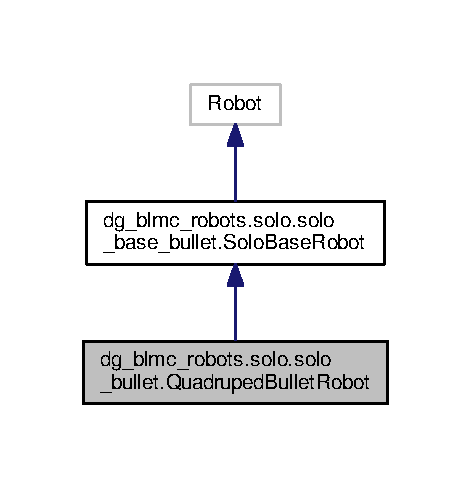
\includegraphics[width=226pt]{classdg__blmc__robots_1_1solo_1_1solo__bullet_1_1QuadrupedBulletRobot__inherit__graph}
\end{center}
\end{figure}


Collaboration diagram for dg\+\_\+blmc\+\_\+robots.\+solo.\+solo\+\_\+bullet.\+Quadruped\+Bullet\+Robot\+:
\nopagebreak
\begin{figure}[H]
\begin{center}
\leavevmode
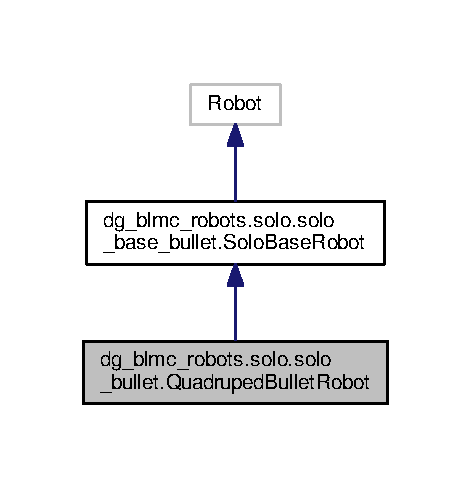
\includegraphics[width=226pt]{classdg__blmc__robots_1_1solo_1_1solo__bullet_1_1QuadrupedBulletRobot__coll__graph}
\end{center}
\end{figure}
\subsection*{Public Member Functions}
\begin{DoxyCompactItemize}
\item 
def {\bfseries \+\_\+\+\_\+init\+\_\+\+\_\+} (self, use\+\_\+fixed\+\_\+base=False, record\+\_\+video=False, init\+\_\+sliders\+\_\+pose=4 $\ast$\mbox{[}0.\+5\mbox{]})\hypertarget{classdg__blmc__robots_1_1solo_1_1solo__bullet_1_1QuadrupedBulletRobot_a7a7cd71aaff5bd10e06b9d750bedf67f}{}\label{classdg__blmc__robots_1_1solo_1_1solo__bullet_1_1QuadrupedBulletRobot_a7a7cd71aaff5bd10e06b9d750bedf67f}

\end{DoxyCompactItemize}
\subsection*{Additional Inherited Members}


The documentation for this class was generated from the following file\+:\begin{DoxyCompactItemize}
\item 
python/dg\+\_\+blmc\+\_\+robots/solo/solo\+\_\+bullet.\+py\end{DoxyCompactItemize}

\hypertarget{classdg__blmc__robots_1_1solo_1_1solo12__bullet_1_1Solo12BulletRobot}{}\section{dg\+\_\+blmc\+\_\+robots.\+solo.\+solo12\+\_\+bullet.\+Solo12\+Bullet\+Robot Class Reference}
\label{classdg__blmc__robots_1_1solo_1_1solo12__bullet_1_1Solo12BulletRobot}\index{dg\+\_\+blmc\+\_\+robots.\+solo.\+solo12\+\_\+bullet.\+Solo12\+Bullet\+Robot@{dg\+\_\+blmc\+\_\+robots.\+solo.\+solo12\+\_\+bullet.\+Solo12\+Bullet\+Robot}}


Inheritance diagram for dg\+\_\+blmc\+\_\+robots.\+solo.\+solo12\+\_\+bullet.\+Solo12\+Bullet\+Robot\+:
\nopagebreak
\begin{figure}[H]
\begin{center}
\leavevmode
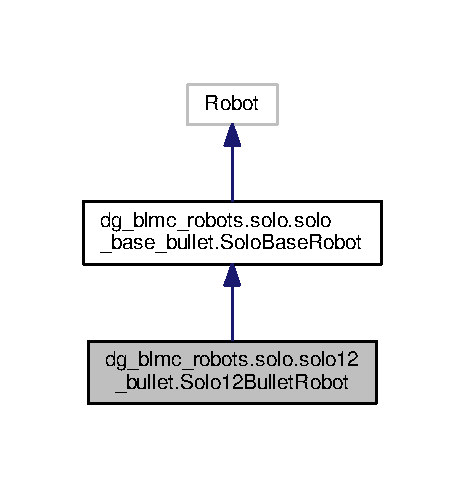
\includegraphics[width=223pt]{classdg__blmc__robots_1_1solo_1_1solo12__bullet_1_1Solo12BulletRobot__inherit__graph}
\end{center}
\end{figure}


Collaboration diagram for dg\+\_\+blmc\+\_\+robots.\+solo.\+solo12\+\_\+bullet.\+Solo12\+Bullet\+Robot\+:
\nopagebreak
\begin{figure}[H]
\begin{center}
\leavevmode
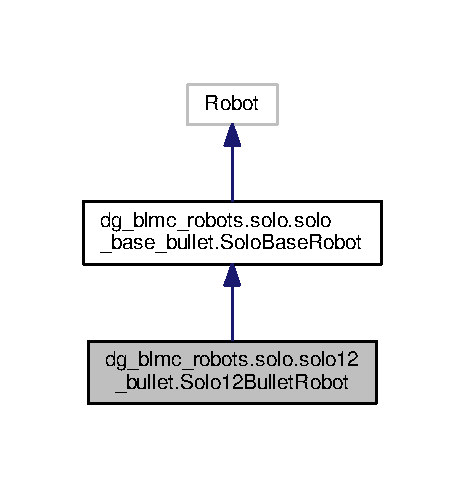
\includegraphics[width=223pt]{classdg__blmc__robots_1_1solo_1_1solo12__bullet_1_1Solo12BulletRobot__coll__graph}
\end{center}
\end{figure}
\subsection*{Public Member Functions}
\begin{DoxyCompactItemize}
\item 
def {\bfseries \+\_\+\+\_\+init\+\_\+\+\_\+} (self, use\+\_\+fixed\+\_\+base=False, record\+\_\+video=False, init\+\_\+sliders\+\_\+pose=4 $\ast$\mbox{[}0.\+5\mbox{]})\hypertarget{classdg__blmc__robots_1_1solo_1_1solo12__bullet_1_1Solo12BulletRobot_abff37cab7c1afded70506629b631af73}{}\label{classdg__blmc__robots_1_1solo_1_1solo12__bullet_1_1Solo12BulletRobot_abff37cab7c1afded70506629b631af73}

\end{DoxyCompactItemize}
\subsection*{Additional Inherited Members}


The documentation for this class was generated from the following file\+:\begin{DoxyCompactItemize}
\item 
python/dg\+\_\+blmc\+\_\+robots/solo/solo12\+\_\+bullet.\+py\end{DoxyCompactItemize}

\hypertarget{classdg__blmc__robots_1_1solo_1_1solo__base__bullet_1_1SoloBaseRobot}{}\section{dg\+\_\+blmc\+\_\+robots.\+solo.\+solo\+\_\+base\+\_\+bullet.\+Solo\+Base\+Robot Class Reference}
\label{classdg__blmc__robots_1_1solo_1_1solo__base__bullet_1_1SoloBaseRobot}\index{dg\+\_\+blmc\+\_\+robots.\+solo.\+solo\+\_\+base\+\_\+bullet.\+Solo\+Base\+Robot@{dg\+\_\+blmc\+\_\+robots.\+solo.\+solo\+\_\+base\+\_\+bullet.\+Solo\+Base\+Robot}}


Base implementation for solo8 and solo12 robot.  




Inheritance diagram for dg\+\_\+blmc\+\_\+robots.\+solo.\+solo\+\_\+base\+\_\+bullet.\+Solo\+Base\+Robot\+:
\nopagebreak
\begin{figure}[H]
\begin{center}
\leavevmode
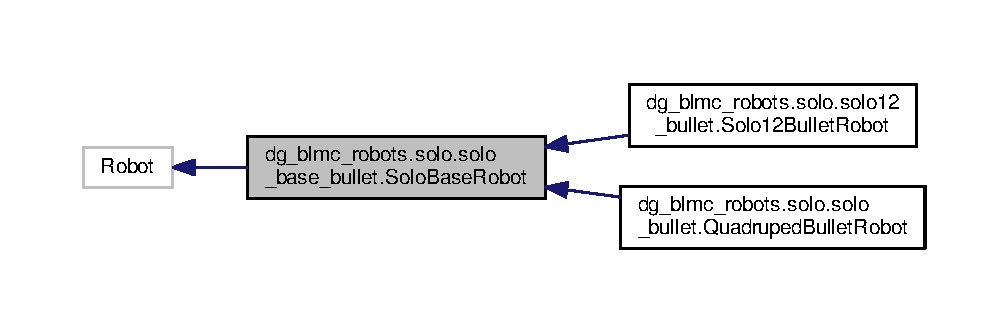
\includegraphics[width=350pt]{classdg__blmc__robots_1_1solo_1_1solo__base__bullet_1_1SoloBaseRobot__inherit__graph}
\end{center}
\end{figure}


Collaboration diagram for dg\+\_\+blmc\+\_\+robots.\+solo.\+solo\+\_\+base\+\_\+bullet.\+Solo\+Base\+Robot\+:
\nopagebreak
\begin{figure}[H]
\begin{center}
\leavevmode
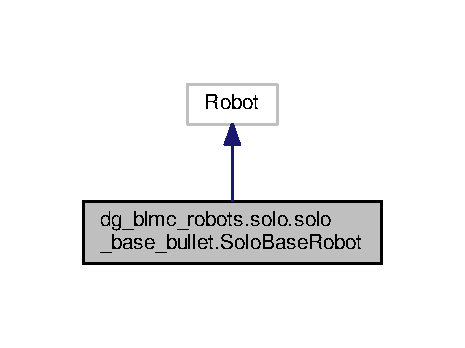
\includegraphics[width=223pt]{classdg__blmc__robots_1_1solo_1_1solo__base__bullet_1_1SoloBaseRobot__coll__graph}
\end{center}
\end{figure}
\subsection*{Public Member Functions}
\begin{DoxyCompactItemize}
\item 
def {\bfseries \+\_\+\+\_\+init\+\_\+\+\_\+} (self, solo\+\_\+config, use\+\_\+fixed\+\_\+base=False, record\+\_\+video=False, init\+\_\+sliders\+\_\+pose=4 $\ast$\mbox{[}0.\+5\mbox{]})\hypertarget{classdg__blmc__robots_1_1solo_1_1solo__base__bullet_1_1SoloBaseRobot_a30831d3a65a139e6bfc5328d214fcd9a}{}\label{classdg__blmc__robots_1_1solo_1_1solo__base__bullet_1_1SoloBaseRobot_a30831d3a65a139e6bfc5328d214fcd9a}

\item 
def {\bfseries pinocchio\+\_\+robot\+\_\+wrapper} (self)\hypertarget{classdg__blmc__robots_1_1solo_1_1solo__base__bullet_1_1SoloBaseRobot_ac0cbf1db601813d147e29d17533ced49}{}\label{classdg__blmc__robots_1_1solo_1_1solo__base__bullet_1_1SoloBaseRobot_ac0cbf1db601813d147e29d17533ced49}

\item 
def {\bfseries base\+\_\+signals} (self)\hypertarget{classdg__blmc__robots_1_1solo_1_1solo__base__bullet_1_1SoloBaseRobot_abdb28c7e04b4a10bdb8d7fd2145337eb}{}\label{classdg__blmc__robots_1_1solo_1_1solo__base__bullet_1_1SoloBaseRobot_abdb28c7e04b4a10bdb8d7fd2145337eb}

\item 
def \hyperlink{classdg__blmc__robots_1_1solo_1_1solo__base__bullet_1_1SoloBaseRobot_aec775b51651007698dde474e4ff5a573}{sim2signal\+\_\+} (self)
\begin{DoxyCompactList}\small\item\em Reads the state from the simulator and fills the corresponding signals. \end{DoxyCompactList}\item 
def {\bfseries run} (self, steps=1, delay=0., plot=False)\hypertarget{classdg__blmc__robots_1_1solo_1_1solo__base__bullet_1_1SoloBaseRobot_a18e7c652d6afa110ce4bd20c655de551}{}\label{classdg__blmc__robots_1_1solo_1_1solo__base__bullet_1_1SoloBaseRobot_a18e7c652d6afa110ce4bd20c655de551}

\item 
def \hyperlink{classdg__blmc__robots_1_1solo_1_1solo__base__bullet_1_1SoloBaseRobot_af007664c1b5587db59a8ac8f5507fdc7}{reset\+\_\+state} (self, q, dq)
\begin{DoxyCompactList}\small\item\em Sets the bullet simulator and the signals to the provided state values. \end{DoxyCompactList}\item 
def \hyperlink{classdg__blmc__robots_1_1solo_1_1solo__base__bullet_1_1SoloBaseRobot_a57f5595c15e6c4382da54ac0e42370aa}{set\+\_\+gravity} (self, vec)
\begin{DoxyCompactList}\small\item\em Sets gravity in the simulator to (x,y,z), where z is the vertical axis. \end{DoxyCompactList}\item 
def {\bfseries print\+\_\+physics\+\_\+engine\+\_\+params} (self)\hypertarget{classdg__blmc__robots_1_1solo_1_1solo__base__bullet_1_1SoloBaseRobot_a600c906596d52aaaba4041f8371e59c7}{}\label{classdg__blmc__robots_1_1solo_1_1solo__base__bullet_1_1SoloBaseRobot_a600c906596d52aaaba4041f8371e59c7}

\item 
def {\bfseries print\+\_\+physics\+\_\+params} (self)\hypertarget{classdg__blmc__robots_1_1solo_1_1solo__base__bullet_1_1SoloBaseRobot_a91fff8ec09cce6d42012fc61d9f1d074}{}\label{classdg__blmc__robots_1_1solo_1_1solo__base__bullet_1_1SoloBaseRobot_a91fff8ec09cce6d42012fc61d9f1d074}

\item 
def {\bfseries add\+\_\+ros\+\_\+and\+\_\+trace} (self, client\+\_\+name, \hyperlink{classdg__blmc__robots_1_1solo_1_1solo__base__bullet_1_1SoloBaseRobot_ae7996643d55ee9abe0a7a844cdd64177}{signal\+\_\+name})\hypertarget{classdg__blmc__robots_1_1solo_1_1solo__base__bullet_1_1SoloBaseRobot_a8c63f4f8b1e18eb73e9e919347b78e28}{}\label{classdg__blmc__robots_1_1solo_1_1solo__base__bullet_1_1SoloBaseRobot_a8c63f4f8b1e18eb73e9e919347b78e28}

\end{DoxyCompactItemize}
\subsection*{Public Attributes}
\begin{DoxyCompactItemize}
\item 
{\bfseries config}\hypertarget{classdg__blmc__robots_1_1solo_1_1solo__base__bullet_1_1SoloBaseRobot_a7b57ece4a23fe5085150e0cb14afdafd}{}\label{classdg__blmc__robots_1_1solo_1_1solo__base__bullet_1_1SoloBaseRobot_a7b57ece4a23fe5085150e0cb14afdafd}

\item 
{\bfseries physics\+Client}\hypertarget{classdg__blmc__robots_1_1solo_1_1solo__base__bullet_1_1SoloBaseRobot_ad7031724d743604bf18abe1ef37e1224}{}\label{classdg__blmc__robots_1_1solo_1_1solo__base__bullet_1_1SoloBaseRobot_ad7031724d743604bf18abe1ef37e1224}

\item 
{\bfseries plane\+Id}\hypertarget{classdg__blmc__robots_1_1solo_1_1solo__base__bullet_1_1SoloBaseRobot_ad6af3d8f95cddadc20c2c7630502ade1}{}\label{classdg__blmc__robots_1_1solo_1_1solo__base__bullet_1_1SoloBaseRobot_ad6af3d8f95cddadc20c2c7630502ade1}

\item 
{\bfseries urdf\+\_\+path}\hypertarget{classdg__blmc__robots_1_1solo_1_1solo__base__bullet_1_1SoloBaseRobot_a24c55f53609938471e2d38ffcd5c58bc}{}\label{classdg__blmc__robots_1_1solo_1_1solo__base__bullet_1_1SoloBaseRobot_a24c55f53609938471e2d38ffcd5c58bc}

\item 
{\bfseries robot\+Id}\hypertarget{classdg__blmc__robots_1_1solo_1_1solo__base__bullet_1_1SoloBaseRobot_a3e57f8bc4cc2ef37fdb75794335aba00}{}\label{classdg__blmc__robots_1_1solo_1_1solo__base__bullet_1_1SoloBaseRobot_a3e57f8bc4cc2ef37fdb75794335aba00}

\item 
{\bfseries pin\+\_\+robot}\hypertarget{classdg__blmc__robots_1_1solo_1_1solo__base__bullet_1_1SoloBaseRobot_a4907996ba46cd696fbc4085b0d76e710}{}\label{classdg__blmc__robots_1_1solo_1_1solo__base__bullet_1_1SoloBaseRobot_a4907996ba46cd696fbc4085b0d76e710}

\item 
{\bfseries base\+\_\+link\+\_\+name}\hypertarget{classdg__blmc__robots_1_1solo_1_1solo__base__bullet_1_1SoloBaseRobot_a4c4d2bcdd88a831db56d93ae86b6247b}{}\label{classdg__blmc__robots_1_1solo_1_1solo__base__bullet_1_1SoloBaseRobot_a4c4d2bcdd88a831db56d93ae86b6247b}

\item 
{\bfseries joint\+\_\+names}\hypertarget{classdg__blmc__robots_1_1solo_1_1solo__base__bullet_1_1SoloBaseRobot_a691ad49984a14ee66625f2910cbe676e}{}\label{classdg__blmc__robots_1_1solo_1_1solo__base__bullet_1_1SoloBaseRobot_a691ad49984a14ee66625f2910cbe676e}

\item 
{\bfseries end\+\_\+effector\+\_\+names}\hypertarget{classdg__blmc__robots_1_1solo_1_1solo__base__bullet_1_1SoloBaseRobot_af429c4b253acf4b30ab8585bff42ff56}{}\label{classdg__blmc__robots_1_1solo_1_1solo__base__bullet_1_1SoloBaseRobot_af429c4b253acf4b30ab8585bff42ff56}

\item 
{\bfseries wrapper}\hypertarget{classdg__blmc__robots_1_1solo_1_1solo__base__bullet_1_1SoloBaseRobot_aafc172390893887571e991b65b0a8470}{}\label{classdg__blmc__robots_1_1solo_1_1solo__base__bullet_1_1SoloBaseRobot_aafc172390893887571e991b65b0a8470}

\item 
{\bfseries slider\+\_\+a}\hypertarget{classdg__blmc__robots_1_1solo_1_1solo__base__bullet_1_1SoloBaseRobot_ad5d11a64741a2b9e9bce65c5377d392d}{}\label{classdg__blmc__robots_1_1solo_1_1solo__base__bullet_1_1SoloBaseRobot_ad5d11a64741a2b9e9bce65c5377d392d}

\item 
{\bfseries slider\+\_\+b}\hypertarget{classdg__blmc__robots_1_1solo_1_1solo__base__bullet_1_1SoloBaseRobot_a06c5b37ea5860b9343440ff8e041c5dd}{}\label{classdg__blmc__robots_1_1solo_1_1solo__base__bullet_1_1SoloBaseRobot_a06c5b37ea5860b9343440ff8e041c5dd}

\item 
{\bfseries slider\+\_\+c}\hypertarget{classdg__blmc__robots_1_1solo_1_1solo__base__bullet_1_1SoloBaseRobot_a7f5bb9abaff5fc82e3c07d341cdc196f}{}\label{classdg__blmc__robots_1_1solo_1_1solo__base__bullet_1_1SoloBaseRobot_a7f5bb9abaff5fc82e3c07d341cdc196f}

\item 
{\bfseries slider\+\_\+d}\hypertarget{classdg__blmc__robots_1_1solo_1_1solo__base__bullet_1_1SoloBaseRobot_a162bcfbed4926519dc6153a56aa6b470}{}\label{classdg__blmc__robots_1_1solo_1_1solo__base__bullet_1_1SoloBaseRobot_a162bcfbed4926519dc6153a56aa6b470}

\item 
{\bfseries hl\+\_\+index}\hypertarget{classdg__blmc__robots_1_1solo_1_1solo__base__bullet_1_1SoloBaseRobot_aa1b50d30650a7ca132b601db06abeacf}{}\label{classdg__blmc__robots_1_1solo_1_1solo__base__bullet_1_1SoloBaseRobot_aa1b50d30650a7ca132b601db06abeacf}

\item 
{\bfseries hr\+\_\+index}\hypertarget{classdg__blmc__robots_1_1solo_1_1solo__base__bullet_1_1SoloBaseRobot_ae4f437fff0e290c9ba3d7fa7089cc81f}{}\label{classdg__blmc__robots_1_1solo_1_1solo__base__bullet_1_1SoloBaseRobot_ae4f437fff0e290c9ba3d7fa7089cc81f}

\item 
{\bfseries fl\+\_\+index}\hypertarget{classdg__blmc__robots_1_1solo_1_1solo__base__bullet_1_1SoloBaseRobot_a816f94fbd7663e5ff2a147064226647e}{}\label{classdg__blmc__robots_1_1solo_1_1solo__base__bullet_1_1SoloBaseRobot_a816f94fbd7663e5ff2a147064226647e}

\item 
{\bfseries fr\+\_\+index}\hypertarget{classdg__blmc__robots_1_1solo_1_1solo__base__bullet_1_1SoloBaseRobot_ab8fc23b6ab9a678ed0517a4a6f1860dd}{}\label{classdg__blmc__robots_1_1solo_1_1solo__base__bullet_1_1SoloBaseRobot_ab8fc23b6ab9a678ed0517a4a6f1860dd}

\item 
{\bfseries device}\hypertarget{classdg__blmc__robots_1_1solo_1_1solo__base__bullet_1_1SoloBaseRobot_a971c703d699ffbc61d812e5d914f0698}{}\label{classdg__blmc__robots_1_1solo_1_1solo__base__bullet_1_1SoloBaseRobot_a971c703d699ffbc61d812e5d914f0698}

\item 
{\bfseries signal\+\_\+base\+\_\+pos\+\_\+}\hypertarget{classdg__blmc__robots_1_1solo_1_1solo__base__bullet_1_1SoloBaseRobot_aca460d32eab1a3bd840abc394dfba707}{}\label{classdg__blmc__robots_1_1solo_1_1solo__base__bullet_1_1SoloBaseRobot_aca460d32eab1a3bd840abc394dfba707}

\item 
{\bfseries signal\+\_\+base\+\_\+vel\+\_\+}\hypertarget{classdg__blmc__robots_1_1solo_1_1solo__base__bullet_1_1SoloBaseRobot_aac4c4bff91b447a0e8df80e65b21814e}{}\label{classdg__blmc__robots_1_1solo_1_1solo__base__bullet_1_1SoloBaseRobot_aac4c4bff91b447a0e8df80e65b21814e}

\item 
{\bfseries q0}\hypertarget{classdg__blmc__robots_1_1solo_1_1solo__base__bullet_1_1SoloBaseRobot_a69f98337da076544e3ed4b153293c7bd}{}\label{classdg__blmc__robots_1_1solo_1_1solo__base__bullet_1_1SoloBaseRobot_a69f98337da076544e3ed4b153293c7bd}

\item 
{\bfseries dq0}\hypertarget{classdg__blmc__robots_1_1solo_1_1solo__base__bullet_1_1SoloBaseRobot_a1298137c2d5cfae62fb70891b15e32bf}{}\label{classdg__blmc__robots_1_1solo_1_1solo__base__bullet_1_1SoloBaseRobot_a1298137c2d5cfae62fb70891b15e32bf}

\item 
{\bfseries steps\+\_\+}\hypertarget{classdg__blmc__robots_1_1solo_1_1solo__base__bullet_1_1SoloBaseRobot_a3c8610957228011f2155884f1ee37900}{}\label{classdg__blmc__robots_1_1solo_1_1solo__base__bullet_1_1SoloBaseRobot_a3c8610957228011f2155884f1ee37900}

\item 
\hyperlink{classdg__blmc__robots_1_1solo_1_1solo__base__bullet_1_1SoloBaseRobot_ae7996643d55ee9abe0a7a844cdd64177}{signal\+\_\+name}\hypertarget{classdg__blmc__robots_1_1solo_1_1solo__base__bullet_1_1SoloBaseRobot_ae7996643d55ee9abe0a7a844cdd64177}{}\label{classdg__blmc__robots_1_1solo_1_1solo__base__bullet_1_1SoloBaseRobot_ae7996643d55ee9abe0a7a844cdd64177}

\begin{DoxyCompactList}\small\item\em for vicon entity \end{DoxyCompactList}\end{DoxyCompactItemize}


\subsection{Detailed Description}
Base implementation for solo8 and solo12 robot. 

\subsection{Member Function Documentation}
\index{dg\+\_\+blmc\+\_\+robots\+::solo\+::solo\+\_\+base\+\_\+bullet\+::\+Solo\+Base\+Robot@{dg\+\_\+blmc\+\_\+robots\+::solo\+::solo\+\_\+base\+\_\+bullet\+::\+Solo\+Base\+Robot}!reset\+\_\+state@{reset\+\_\+state}}
\index{reset\+\_\+state@{reset\+\_\+state}!dg\+\_\+blmc\+\_\+robots\+::solo\+::solo\+\_\+base\+\_\+bullet\+::\+Solo\+Base\+Robot@{dg\+\_\+blmc\+\_\+robots\+::solo\+::solo\+\_\+base\+\_\+bullet\+::\+Solo\+Base\+Robot}}
\subsubsection[{\texorpdfstring{reset\+\_\+state(self, q, dq)}{reset_state(self, q, dq)}}]{\setlength{\rightskip}{0pt plus 5cm}def dg\+\_\+blmc\+\_\+robots.\+solo.\+solo\+\_\+base\+\_\+bullet.\+Solo\+Base\+Robot.\+reset\+\_\+state (
\begin{DoxyParamCaption}
\item[{}]{self, }
\item[{}]{q, }
\item[{}]{dq}
\end{DoxyParamCaption}
)}\hypertarget{classdg__blmc__robots_1_1solo_1_1solo__base__bullet_1_1SoloBaseRobot_af007664c1b5587db59a8ac8f5507fdc7}{}\label{classdg__blmc__robots_1_1solo_1_1solo__base__bullet_1_1SoloBaseRobot_af007664c1b5587db59a8ac8f5507fdc7}


Sets the bullet simulator and the signals to the provided state values. 

\index{dg\+\_\+blmc\+\_\+robots\+::solo\+::solo\+\_\+base\+\_\+bullet\+::\+Solo\+Base\+Robot@{dg\+\_\+blmc\+\_\+robots\+::solo\+::solo\+\_\+base\+\_\+bullet\+::\+Solo\+Base\+Robot}!set\+\_\+gravity@{set\+\_\+gravity}}
\index{set\+\_\+gravity@{set\+\_\+gravity}!dg\+\_\+blmc\+\_\+robots\+::solo\+::solo\+\_\+base\+\_\+bullet\+::\+Solo\+Base\+Robot@{dg\+\_\+blmc\+\_\+robots\+::solo\+::solo\+\_\+base\+\_\+bullet\+::\+Solo\+Base\+Robot}}
\subsubsection[{\texorpdfstring{set\+\_\+gravity(self, vec)}{set_gravity(self, vec)}}]{\setlength{\rightskip}{0pt plus 5cm}def dg\+\_\+blmc\+\_\+robots.\+solo.\+solo\+\_\+base\+\_\+bullet.\+Solo\+Base\+Robot.\+set\+\_\+gravity (
\begin{DoxyParamCaption}
\item[{}]{self, }
\item[{}]{vec}
\end{DoxyParamCaption}
)}\hypertarget{classdg__blmc__robots_1_1solo_1_1solo__base__bullet_1_1SoloBaseRobot_a57f5595c15e6c4382da54ac0e42370aa}{}\label{classdg__blmc__robots_1_1solo_1_1solo__base__bullet_1_1SoloBaseRobot_a57f5595c15e6c4382da54ac0e42370aa}


Sets gravity in the simulator to (x,y,z), where z is the vertical axis. 

\index{dg\+\_\+blmc\+\_\+robots\+::solo\+::solo\+\_\+base\+\_\+bullet\+::\+Solo\+Base\+Robot@{dg\+\_\+blmc\+\_\+robots\+::solo\+::solo\+\_\+base\+\_\+bullet\+::\+Solo\+Base\+Robot}!sim2signal\+\_\+@{sim2signal\+\_\+}}
\index{sim2signal\+\_\+@{sim2signal\+\_\+}!dg\+\_\+blmc\+\_\+robots\+::solo\+::solo\+\_\+base\+\_\+bullet\+::\+Solo\+Base\+Robot@{dg\+\_\+blmc\+\_\+robots\+::solo\+::solo\+\_\+base\+\_\+bullet\+::\+Solo\+Base\+Robot}}
\subsubsection[{\texorpdfstring{sim2signal\+\_\+(self)}{sim2signal_(self)}}]{\setlength{\rightskip}{0pt plus 5cm}def dg\+\_\+blmc\+\_\+robots.\+solo.\+solo\+\_\+base\+\_\+bullet.\+Solo\+Base\+Robot.\+sim2signal\+\_\+ (
\begin{DoxyParamCaption}
\item[{}]{self}
\end{DoxyParamCaption}
)}\hypertarget{classdg__blmc__robots_1_1solo_1_1solo__base__bullet_1_1SoloBaseRobot_aec775b51651007698dde474e4ff5a573}{}\label{classdg__blmc__robots_1_1solo_1_1solo__base__bullet_1_1SoloBaseRobot_aec775b51651007698dde474e4ff5a573}


Reads the state from the simulator and fills the corresponding signals. 



The documentation for this class was generated from the following file\+:\begin{DoxyCompactItemize}
\item 
python/dg\+\_\+blmc\+\_\+robots/solo/solo\+\_\+base\+\_\+bullet.\+py\end{DoxyCompactItemize}

\hypertarget{classstuggihop__bullet_1_1StuggihopBulletRobot}{}\section{stuggihop\+\_\+bullet.\+Stuggihop\+Bullet\+Robot Class Reference}
\label{classstuggihop__bullet_1_1StuggihopBulletRobot}\index{stuggihop\+\_\+bullet.\+Stuggihop\+Bullet\+Robot@{stuggihop\+\_\+bullet.\+Stuggihop\+Bullet\+Robot}}


Inheritance diagram for stuggihop\+\_\+bullet.\+Stuggihop\+Bullet\+Robot\+:
\nopagebreak
\begin{figure}[H]
\begin{center}
\leavevmode
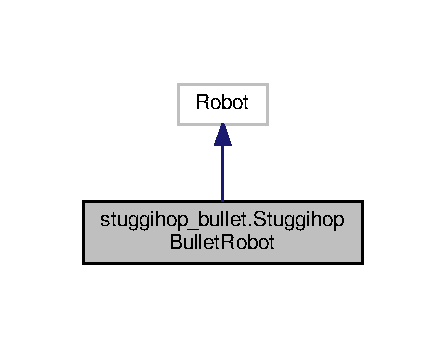
\includegraphics[width=214pt]{classstuggihop__bullet_1_1StuggihopBulletRobot__inherit__graph}
\end{center}
\end{figure}


Collaboration diagram for stuggihop\+\_\+bullet.\+Stuggihop\+Bullet\+Robot\+:
\nopagebreak
\begin{figure}[H]
\begin{center}
\leavevmode
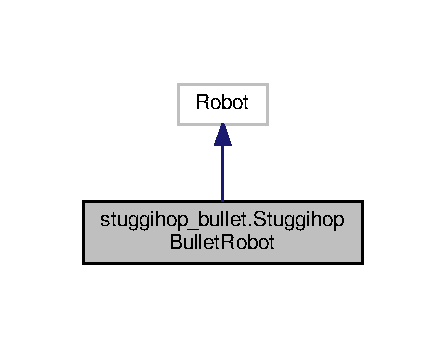
\includegraphics[width=214pt]{classstuggihop__bullet_1_1StuggihopBulletRobot__coll__graph}
\end{center}
\end{figure}
\subsection*{Public Member Functions}
\begin{DoxyCompactItemize}
\item 
def {\bfseries \+\_\+\+\_\+init\+\_\+\+\_\+} (self)\hypertarget{classstuggihop__bullet_1_1StuggihopBulletRobot_a569b29d12262e456dce236bb166b9423}{}\label{classstuggihop__bullet_1_1StuggihopBulletRobot_a569b29d12262e456dce236bb166b9423}

\item 
def {\bfseries pinocchio\+\_\+robot\+\_\+wrapper} (self)\hypertarget{classstuggihop__bullet_1_1StuggihopBulletRobot_abf99ffa6f01c91a753f2c43870f8e923}{}\label{classstuggihop__bullet_1_1StuggihopBulletRobot_abf99ffa6f01c91a753f2c43870f8e923}

\item 
def \hyperlink{classstuggihop__bullet_1_1StuggihopBulletRobot_af75d6c773ccea849139a291173c0af09}{sim2signal\+\_\+} (self)
\begin{DoxyCompactList}\small\item\em Reads the state from the simulator and fills the corresponding signals. \end{DoxyCompactList}\item 
def {\bfseries run} (self, steps=1, delay=0.)\hypertarget{classstuggihop__bullet_1_1StuggihopBulletRobot_a20656822edcbffc313bd06dca182dcc4}{}\label{classstuggihop__bullet_1_1StuggihopBulletRobot_a20656822edcbffc313bd06dca182dcc4}

\item 
def \hyperlink{classstuggihop__bullet_1_1StuggihopBulletRobot_aea04a3ddb2665ed7aa19c81206c95bf7}{reset\+\_\+state} (self, q, dq)
\begin{DoxyCompactList}\small\item\em Sets the bullet simulator and the signals to the provided state values. \end{DoxyCompactList}\item 
def \hyperlink{classstuggihop__bullet_1_1StuggihopBulletRobot_ae497030ea6a7849f0a6bd6fb881f3935}{set\+\_\+gravity} (self, vec)
\begin{DoxyCompactList}\small\item\em Sets gravity in the simulator to (x,y,z), where z is the vertical axis. \end{DoxyCompactList}\end{DoxyCompactItemize}
\subsection*{Public Attributes}
\begin{DoxyCompactItemize}
\item 
{\bfseries physics\+Client}\hypertarget{classstuggihop__bullet_1_1StuggihopBulletRobot_adb65069912552a6965de216f00b90fd1}{}\label{classstuggihop__bullet_1_1StuggihopBulletRobot_adb65069912552a6965de216f00b90fd1}

\item 
{\bfseries plane\+Id}\hypertarget{classstuggihop__bullet_1_1StuggihopBulletRobot_a5f2633e92b6b3e436506a013130883a4}{}\label{classstuggihop__bullet_1_1StuggihopBulletRobot_a5f2633e92b6b3e436506a013130883a4}

\item 
{\bfseries urdf\+\_\+path}\hypertarget{classstuggihop__bullet_1_1StuggihopBulletRobot_a3b15c6b3034759600cbeac8e032d9399}{}\label{classstuggihop__bullet_1_1StuggihopBulletRobot_a3b15c6b3034759600cbeac8e032d9399}

\item 
{\bfseries robot\+Id}\hypertarget{classstuggihop__bullet_1_1StuggihopBulletRobot_ae60b1846bc5e43f4f7128b56db2c7b54}{}\label{classstuggihop__bullet_1_1StuggihopBulletRobot_ae60b1846bc5e43f4f7128b56db2c7b54}

\item 
{\bfseries pin\+\_\+robot}\hypertarget{classstuggihop__bullet_1_1StuggihopBulletRobot_af545fbec7bccee36c4d5013855bef6cc}{}\label{classstuggihop__bullet_1_1StuggihopBulletRobot_af545fbec7bccee36c4d5013855bef6cc}

\item 
{\bfseries joint\+\_\+names}\hypertarget{classstuggihop__bullet_1_1StuggihopBulletRobot_a2fbaabbf4de99f16a713447f0b670c6b}{}\label{classstuggihop__bullet_1_1StuggihopBulletRobot_a2fbaabbf4de99f16a713447f0b670c6b}

\item 
{\bfseries wrapper}\hypertarget{classstuggihop__bullet_1_1StuggihopBulletRobot_a22182836b54d5b885b004bd423361ef8}{}\label{classstuggihop__bullet_1_1StuggihopBulletRobot_a22182836b54d5b885b004bd423361ef8}

\item 
{\bfseries device}\hypertarget{classstuggihop__bullet_1_1StuggihopBulletRobot_a0f035485d9a2c506839c4917b5b27daf}{}\label{classstuggihop__bullet_1_1StuggihopBulletRobot_a0f035485d9a2c506839c4917b5b27daf}

\item 
{\bfseries steps\+\_\+}\hypertarget{classstuggihop__bullet_1_1StuggihopBulletRobot_a891f4a1c2e0cebdcdfe6b6e4963b97c0}{}\label{classstuggihop__bullet_1_1StuggihopBulletRobot_a891f4a1c2e0cebdcdfe6b6e4963b97c0}

\end{DoxyCompactItemize}


\subsection{Member Function Documentation}
\index{stuggihop\+\_\+bullet\+::\+Stuggihop\+Bullet\+Robot@{stuggihop\+\_\+bullet\+::\+Stuggihop\+Bullet\+Robot}!reset\+\_\+state@{reset\+\_\+state}}
\index{reset\+\_\+state@{reset\+\_\+state}!stuggihop\+\_\+bullet\+::\+Stuggihop\+Bullet\+Robot@{stuggihop\+\_\+bullet\+::\+Stuggihop\+Bullet\+Robot}}
\subsubsection[{\texorpdfstring{reset\+\_\+state(self, q, dq)}{reset_state(self, q, dq)}}]{\setlength{\rightskip}{0pt plus 5cm}def stuggihop\+\_\+bullet.\+Stuggihop\+Bullet\+Robot.\+reset\+\_\+state (
\begin{DoxyParamCaption}
\item[{}]{self, }
\item[{}]{q, }
\item[{}]{dq}
\end{DoxyParamCaption}
)}\hypertarget{classstuggihop__bullet_1_1StuggihopBulletRobot_aea04a3ddb2665ed7aa19c81206c95bf7}{}\label{classstuggihop__bullet_1_1StuggihopBulletRobot_aea04a3ddb2665ed7aa19c81206c95bf7}


Sets the bullet simulator and the signals to the provided state values. 

\index{stuggihop\+\_\+bullet\+::\+Stuggihop\+Bullet\+Robot@{stuggihop\+\_\+bullet\+::\+Stuggihop\+Bullet\+Robot}!set\+\_\+gravity@{set\+\_\+gravity}}
\index{set\+\_\+gravity@{set\+\_\+gravity}!stuggihop\+\_\+bullet\+::\+Stuggihop\+Bullet\+Robot@{stuggihop\+\_\+bullet\+::\+Stuggihop\+Bullet\+Robot}}
\subsubsection[{\texorpdfstring{set\+\_\+gravity(self, vec)}{set_gravity(self, vec)}}]{\setlength{\rightskip}{0pt plus 5cm}def stuggihop\+\_\+bullet.\+Stuggihop\+Bullet\+Robot.\+set\+\_\+gravity (
\begin{DoxyParamCaption}
\item[{}]{self, }
\item[{}]{vec}
\end{DoxyParamCaption}
)}\hypertarget{classstuggihop__bullet_1_1StuggihopBulletRobot_ae497030ea6a7849f0a6bd6fb881f3935}{}\label{classstuggihop__bullet_1_1StuggihopBulletRobot_ae497030ea6a7849f0a6bd6fb881f3935}


Sets gravity in the simulator to (x,y,z), where z is the vertical axis. 

\index{stuggihop\+\_\+bullet\+::\+Stuggihop\+Bullet\+Robot@{stuggihop\+\_\+bullet\+::\+Stuggihop\+Bullet\+Robot}!sim2signal\+\_\+@{sim2signal\+\_\+}}
\index{sim2signal\+\_\+@{sim2signal\+\_\+}!stuggihop\+\_\+bullet\+::\+Stuggihop\+Bullet\+Robot@{stuggihop\+\_\+bullet\+::\+Stuggihop\+Bullet\+Robot}}
\subsubsection[{\texorpdfstring{sim2signal\+\_\+(self)}{sim2signal_(self)}}]{\setlength{\rightskip}{0pt plus 5cm}def stuggihop\+\_\+bullet.\+Stuggihop\+Bullet\+Robot.\+sim2signal\+\_\+ (
\begin{DoxyParamCaption}
\item[{}]{self}
\end{DoxyParamCaption}
)}\hypertarget{classstuggihop__bullet_1_1StuggihopBulletRobot_af75d6c773ccea849139a291173c0af09}{}\label{classstuggihop__bullet_1_1StuggihopBulletRobot_af75d6c773ccea849139a291173c0af09}


Reads the state from the simulator and fills the corresponding signals. 



The documentation for this class was generated from the following file\+:\begin{DoxyCompactItemize}
\item 
python/dg\+\_\+blmc\+\_\+robots/stuggihop/stuggihop\+\_\+bullet.\+py\end{DoxyCompactItemize}

\hypertarget{classdg__blmc__robots_1_1teststand_1_1teststand__bullet_1_1TeststandBulletRobot}{}\section{dg\+\_\+blmc\+\_\+robots.\+teststand.\+teststand\+\_\+bullet.\+Teststand\+Bullet\+Robot Class Reference}
\label{classdg__blmc__robots_1_1teststand_1_1teststand__bullet_1_1TeststandBulletRobot}\index{dg\+\_\+blmc\+\_\+robots.\+teststand.\+teststand\+\_\+bullet.\+Teststand\+Bullet\+Robot@{dg\+\_\+blmc\+\_\+robots.\+teststand.\+teststand\+\_\+bullet.\+Teststand\+Bullet\+Robot}}


Inheritance diagram for dg\+\_\+blmc\+\_\+robots.\+teststand.\+teststand\+\_\+bullet.\+Teststand\+Bullet\+Robot\+:
\nopagebreak
\begin{figure}[H]
\begin{center}
\leavevmode
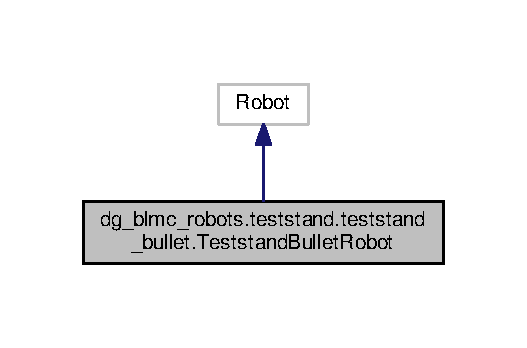
\includegraphics[width=253pt]{classdg__blmc__robots_1_1teststand_1_1teststand__bullet_1_1TeststandBulletRobot__inherit__graph}
\end{center}
\end{figure}


Collaboration diagram for dg\+\_\+blmc\+\_\+robots.\+teststand.\+teststand\+\_\+bullet.\+Teststand\+Bullet\+Robot\+:
\nopagebreak
\begin{figure}[H]
\begin{center}
\leavevmode
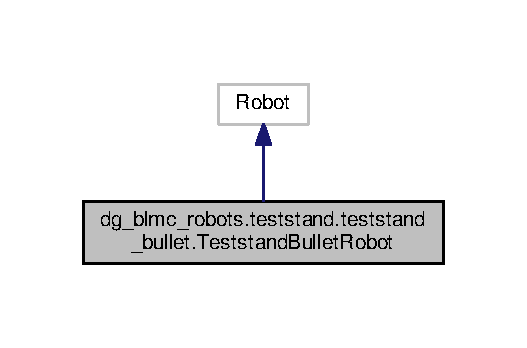
\includegraphics[width=253pt]{classdg__blmc__robots_1_1teststand_1_1teststand__bullet_1_1TeststandBulletRobot__coll__graph}
\end{center}
\end{figure}
\subsection*{Public Member Functions}
\begin{DoxyCompactItemize}
\item 
def {\bfseries \+\_\+\+\_\+init\+\_\+\+\_\+} (self, fixed\+\_\+slider, init\+\_\+sliders\+\_\+pose, with\+\_\+gui)\hypertarget{classdg__blmc__robots_1_1teststand_1_1teststand__bullet_1_1TeststandBulletRobot_aed7733bebc63fa65d527ae2bfe133b9a}{}\label{classdg__blmc__robots_1_1teststand_1_1teststand__bullet_1_1TeststandBulletRobot_aed7733bebc63fa65d527ae2bfe133b9a}

\item 
def {\bfseries pinocchio\+\_\+robot\+\_\+wrapper} (self)\hypertarget{classdg__blmc__robots_1_1teststand_1_1teststand__bullet_1_1TeststandBulletRobot_a4062815d510c246c8a9b7b38b11f8fbc}{}\label{classdg__blmc__robots_1_1teststand_1_1teststand__bullet_1_1TeststandBulletRobot_a4062815d510c246c8a9b7b38b11f8fbc}

\item 
def \hyperlink{classdg__blmc__robots_1_1teststand_1_1teststand__bullet_1_1TeststandBulletRobot_a961e8a9d4f6cc368503cf0923eb80940}{set\+\_\+gravity} (self, vec)
\begin{DoxyCompactList}\small\item\em Sets gravity in the simulator to (x,y,z), where z is the vertical axis. \end{DoxyCompactList}\item 
def {\bfseries run} (self, steps=1, delay=0.)\hypertarget{classdg__blmc__robots_1_1teststand_1_1teststand__bullet_1_1TeststandBulletRobot_a64326376acc832babc838f6d0f2499e8}{}\label{classdg__blmc__robots_1_1teststand_1_1teststand__bullet_1_1TeststandBulletRobot_a64326376acc832babc838f6d0f2499e8}

\item 
def \hyperlink{classdg__blmc__robots_1_1teststand_1_1teststand__bullet_1_1TeststandBulletRobot_acbb1f3051c8d20cd8fec0126f3b93246}{reset\+\_\+state} (self, q, dq)
\begin{DoxyCompactList}\small\item\em Sets the bullet simulator and the signals to the provided state values. \end{DoxyCompactList}\end{DoxyCompactItemize}
\subsection*{Public Attributes}
\begin{DoxyCompactItemize}
\item 
{\bfseries fixed\+\_\+slider}\hypertarget{classdg__blmc__robots_1_1teststand_1_1teststand__bullet_1_1TeststandBulletRobot_a72fb05a7d46ebb4ff27d3128bd165e6a}{}\label{classdg__blmc__robots_1_1teststand_1_1teststand__bullet_1_1TeststandBulletRobot_a72fb05a7d46ebb4ff27d3128bd165e6a}

\item 
{\bfseries init\+\_\+sliders\+\_\+pose}\hypertarget{classdg__blmc__robots_1_1teststand_1_1teststand__bullet_1_1TeststandBulletRobot_a8000b9e8e4cb2580d7b32cd1604e30af}{}\label{classdg__blmc__robots_1_1teststand_1_1teststand__bullet_1_1TeststandBulletRobot_a8000b9e8e4cb2580d7b32cd1604e30af}

\item 
{\bfseries with\+\_\+gui}\hypertarget{classdg__blmc__robots_1_1teststand_1_1teststand__bullet_1_1TeststandBulletRobot_af48eb5373eea09d49f43ed41bf136718}{}\label{classdg__blmc__robots_1_1teststand_1_1teststand__bullet_1_1TeststandBulletRobot_af48eb5373eea09d49f43ed41bf136718}

\item 
{\bfseries physics\+Client}\hypertarget{classdg__blmc__robots_1_1teststand_1_1teststand__bullet_1_1TeststandBulletRobot_ae1f8bcfbc31914de23c001a8385db55c}{}\label{classdg__blmc__robots_1_1teststand_1_1teststand__bullet_1_1TeststandBulletRobot_ae1f8bcfbc31914de23c001a8385db55c}

\item 
{\bfseries slider\+\_\+a}\hypertarget{classdg__blmc__robots_1_1teststand_1_1teststand__bullet_1_1TeststandBulletRobot_abeead6eed290841a0f23e463f222c8a2}{}\label{classdg__blmc__robots_1_1teststand_1_1teststand__bullet_1_1TeststandBulletRobot_abeead6eed290841a0f23e463f222c8a2}

\item 
{\bfseries slider\+\_\+b}\hypertarget{classdg__blmc__robots_1_1teststand_1_1teststand__bullet_1_1TeststandBulletRobot_ae561f96679a7e42756118c49797fb7e4}{}\label{classdg__blmc__robots_1_1teststand_1_1teststand__bullet_1_1TeststandBulletRobot_ae561f96679a7e42756118c49797fb7e4}

\item 
{\bfseries plane\+Id}\hypertarget{classdg__blmc__robots_1_1teststand_1_1teststand__bullet_1_1TeststandBulletRobot_ae2ea7111ebbbd7a644f16908331d4edb}{}\label{classdg__blmc__robots_1_1teststand_1_1teststand__bullet_1_1TeststandBulletRobot_ae2ea7111ebbbd7a644f16908331d4edb}

\item 
{\bfseries config}\hypertarget{classdg__blmc__robots_1_1teststand_1_1teststand__bullet_1_1TeststandBulletRobot_a9a6c49f19531ebcb9772611e47c0ac25}{}\label{classdg__blmc__robots_1_1teststand_1_1teststand__bullet_1_1TeststandBulletRobot_a9a6c49f19531ebcb9772611e47c0ac25}

\item 
{\bfseries urdf\+\_\+path}\hypertarget{classdg__blmc__robots_1_1teststand_1_1teststand__bullet_1_1TeststandBulletRobot_a8c5323f16b7516e4f20cd03431e9f3b5}{}\label{classdg__blmc__robots_1_1teststand_1_1teststand__bullet_1_1TeststandBulletRobot_a8c5323f16b7516e4f20cd03431e9f3b5}

\item 
{\bfseries robot\+Id}\hypertarget{classdg__blmc__robots_1_1teststand_1_1teststand__bullet_1_1TeststandBulletRobot_a677db589110efcd9e99007db20326e1a}{}\label{classdg__blmc__robots_1_1teststand_1_1teststand__bullet_1_1TeststandBulletRobot_a677db589110efcd9e99007db20326e1a}

\item 
{\bfseries pin\+\_\+robot}\hypertarget{classdg__blmc__robots_1_1teststand_1_1teststand__bullet_1_1TeststandBulletRobot_ac3ae4d5955819b1ffa14c54f7f7ee8b9}{}\label{classdg__blmc__robots_1_1teststand_1_1teststand__bullet_1_1TeststandBulletRobot_ac3ae4d5955819b1ffa14c54f7f7ee8b9}

\item 
{\bfseries joint\+\_\+names}\hypertarget{classdg__blmc__robots_1_1teststand_1_1teststand__bullet_1_1TeststandBulletRobot_a06a423742febadfa202356523de626d1}{}\label{classdg__blmc__robots_1_1teststand_1_1teststand__bullet_1_1TeststandBulletRobot_a06a423742febadfa202356523de626d1}

\item 
{\bfseries wrapper}\hypertarget{classdg__blmc__robots_1_1teststand_1_1teststand__bullet_1_1TeststandBulletRobot_a92172d6acfecf491fbe7e058e8f0a60d}{}\label{classdg__blmc__robots_1_1teststand_1_1teststand__bullet_1_1TeststandBulletRobot_a92172d6acfecf491fbe7e058e8f0a60d}

\item 
{\bfseries device}\hypertarget{classdg__blmc__robots_1_1teststand_1_1teststand__bullet_1_1TeststandBulletRobot_aa13bccdb2104a27dee593452c555a167}{}\label{classdg__blmc__robots_1_1teststand_1_1teststand__bullet_1_1TeststandBulletRobot_aa13bccdb2104a27dee593452c555a167}

\item 
{\bfseries steps\+\_\+}\hypertarget{classdg__blmc__robots_1_1teststand_1_1teststand__bullet_1_1TeststandBulletRobot_a053df91390594bb787c118637a2e7676}{}\label{classdg__blmc__robots_1_1teststand_1_1teststand__bullet_1_1TeststandBulletRobot_a053df91390594bb787c118637a2e7676}

\end{DoxyCompactItemize}
\subsection*{Private Member Functions}
\begin{DoxyCompactItemize}
\item 
def \hyperlink{classdg__blmc__robots_1_1teststand_1_1teststand__bullet_1_1TeststandBulletRobot_aff24fbcd5ded6221c7c666affd0bf613}{\+\_\+sim2signal} (self)\hypertarget{classdg__blmc__robots_1_1teststand_1_1teststand__bullet_1_1TeststandBulletRobot_aff24fbcd5ded6221c7c666affd0bf613}{}\label{classdg__blmc__robots_1_1teststand_1_1teststand__bullet_1_1TeststandBulletRobot_aff24fbcd5ded6221c7c666affd0bf613}

\begin{DoxyCompactList}\small\item\em Reads the state from the simulator and fills the corresponding signals. \end{DoxyCompactList}\end{DoxyCompactItemize}


\subsection{Member Function Documentation}
\index{dg\+\_\+blmc\+\_\+robots\+::teststand\+::teststand\+\_\+bullet\+::\+Teststand\+Bullet\+Robot@{dg\+\_\+blmc\+\_\+robots\+::teststand\+::teststand\+\_\+bullet\+::\+Teststand\+Bullet\+Robot}!reset\+\_\+state@{reset\+\_\+state}}
\index{reset\+\_\+state@{reset\+\_\+state}!dg\+\_\+blmc\+\_\+robots\+::teststand\+::teststand\+\_\+bullet\+::\+Teststand\+Bullet\+Robot@{dg\+\_\+blmc\+\_\+robots\+::teststand\+::teststand\+\_\+bullet\+::\+Teststand\+Bullet\+Robot}}
\subsubsection[{\texorpdfstring{reset\+\_\+state(self, q, dq)}{reset_state(self, q, dq)}}]{\setlength{\rightskip}{0pt plus 5cm}def dg\+\_\+blmc\+\_\+robots.\+teststand.\+teststand\+\_\+bullet.\+Teststand\+Bullet\+Robot.\+reset\+\_\+state (
\begin{DoxyParamCaption}
\item[{}]{self, }
\item[{}]{q, }
\item[{}]{dq}
\end{DoxyParamCaption}
)}\hypertarget{classdg__blmc__robots_1_1teststand_1_1teststand__bullet_1_1TeststandBulletRobot_acbb1f3051c8d20cd8fec0126f3b93246}{}\label{classdg__blmc__robots_1_1teststand_1_1teststand__bullet_1_1TeststandBulletRobot_acbb1f3051c8d20cd8fec0126f3b93246}


Sets the bullet simulator and the signals to the provided state values. 

\index{dg\+\_\+blmc\+\_\+robots\+::teststand\+::teststand\+\_\+bullet\+::\+Teststand\+Bullet\+Robot@{dg\+\_\+blmc\+\_\+robots\+::teststand\+::teststand\+\_\+bullet\+::\+Teststand\+Bullet\+Robot}!set\+\_\+gravity@{set\+\_\+gravity}}
\index{set\+\_\+gravity@{set\+\_\+gravity}!dg\+\_\+blmc\+\_\+robots\+::teststand\+::teststand\+\_\+bullet\+::\+Teststand\+Bullet\+Robot@{dg\+\_\+blmc\+\_\+robots\+::teststand\+::teststand\+\_\+bullet\+::\+Teststand\+Bullet\+Robot}}
\subsubsection[{\texorpdfstring{set\+\_\+gravity(self, vec)}{set_gravity(self, vec)}}]{\setlength{\rightskip}{0pt plus 5cm}def dg\+\_\+blmc\+\_\+robots.\+teststand.\+teststand\+\_\+bullet.\+Teststand\+Bullet\+Robot.\+set\+\_\+gravity (
\begin{DoxyParamCaption}
\item[{}]{self, }
\item[{}]{vec}
\end{DoxyParamCaption}
)}\hypertarget{classdg__blmc__robots_1_1teststand_1_1teststand__bullet_1_1TeststandBulletRobot_a961e8a9d4f6cc368503cf0923eb80940}{}\label{classdg__blmc__robots_1_1teststand_1_1teststand__bullet_1_1TeststandBulletRobot_a961e8a9d4f6cc368503cf0923eb80940}


Sets gravity in the simulator to (x,y,z), where z is the vertical axis. 



The documentation for this class was generated from the following file\+:\begin{DoxyCompactItemize}
\item 
python/dg\+\_\+blmc\+\_\+robots/teststand/teststand\+\_\+bullet.\+py\end{DoxyCompactItemize}

\hypertarget{classdg__blmc__robots_1_1vicon__client__bullet_1_1ViconClientEntityBullet}{}\section{dg\+\_\+blmc\+\_\+robots.\+vicon\+\_\+client\+\_\+bullet.\+Vicon\+Client\+Entity\+Bullet Class Reference}
\label{classdg__blmc__robots_1_1vicon__client__bullet_1_1ViconClientEntityBullet}\index{dg\+\_\+blmc\+\_\+robots.\+vicon\+\_\+client\+\_\+bullet.\+Vicon\+Client\+Entity\+Bullet@{dg\+\_\+blmc\+\_\+robots.\+vicon\+\_\+client\+\_\+bullet.\+Vicon\+Client\+Entity\+Bullet}}


Viconclient object for center of mass control.  




Inheritance diagram for dg\+\_\+blmc\+\_\+robots.\+vicon\+\_\+client\+\_\+bullet.\+Vicon\+Client\+Entity\+Bullet\+:
\nopagebreak
\begin{figure}[H]
\begin{center}
\leavevmode
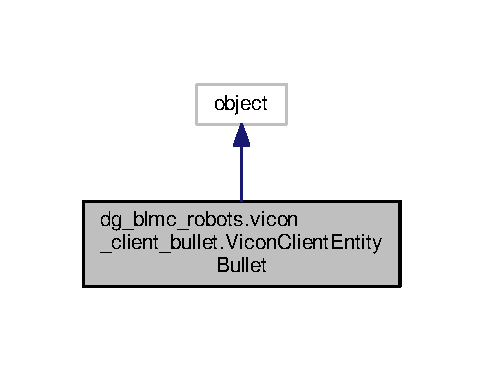
\includegraphics[width=232pt]{classdg__blmc__robots_1_1vicon__client__bullet_1_1ViconClientEntityBullet__inherit__graph}
\end{center}
\end{figure}


Collaboration diagram for dg\+\_\+blmc\+\_\+robots.\+vicon\+\_\+client\+\_\+bullet.\+Vicon\+Client\+Entity\+Bullet\+:
\nopagebreak
\begin{figure}[H]
\begin{center}
\leavevmode
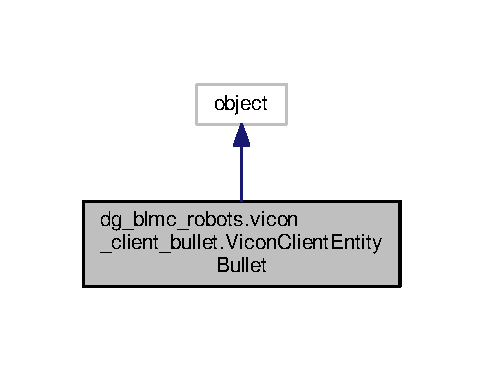
\includegraphics[width=232pt]{classdg__blmc__robots_1_1vicon__client__bullet_1_1ViconClientEntityBullet__coll__graph}
\end{center}
\end{figure}
\subsection*{Public Member Functions}
\begin{DoxyCompactItemize}
\item 
def {\bfseries \+\_\+\+\_\+init\+\_\+\+\_\+} (self, client\+Name)\hypertarget{classdg__blmc__robots_1_1vicon__client__bullet_1_1ViconClientEntityBullet_abd17b337138290f9f3c6abd34ac2cd53}{}\label{classdg__blmc__robots_1_1vicon__client__bullet_1_1ViconClientEntityBullet_abd17b337138290f9f3c6abd34ac2cd53}

\item 
def {\bfseries connect\+\_\+to\+\_\+vicon} (self, host\+\_\+name)\hypertarget{classdg__blmc__robots_1_1vicon__client__bullet_1_1ViconClientEntityBullet_a2124aec6b0a1fbf46384da27592d0ed5}{}\label{classdg__blmc__robots_1_1vicon__client__bullet_1_1ViconClientEntityBullet_a2124aec6b0a1fbf46384da27592d0ed5}

\item 
def {\bfseries display\+Signals} (self)\hypertarget{classdg__blmc__robots_1_1vicon__client__bullet_1_1ViconClientEntityBullet_afdf5d88a0ee499f5130832dfc802274d}{}\label{classdg__blmc__robots_1_1vicon__client__bullet_1_1ViconClientEntityBullet_afdf5d88a0ee499f5130832dfc802274d}

\item 
def {\bfseries add\+\_\+object\+\_\+to\+\_\+track} (self, name)\hypertarget{classdg__blmc__robots_1_1vicon__client__bullet_1_1ViconClientEntityBullet_a93269b2f385b01a0b0c72aef9a592ff7}{}\label{classdg__blmc__robots_1_1vicon__client__bullet_1_1ViconClientEntityBullet_a93269b2f385b01a0b0c72aef9a592ff7}

\item 
def {\bfseries robot\+\_\+wrapper} (self, robot\+\_\+wrapper, robot\+\_\+vicon\+\_\+name)\hypertarget{classdg__blmc__robots_1_1vicon__client__bullet_1_1ViconClientEntityBullet_a2bb0457c535787ffb3c90afaee5f5f7e}{}\label{classdg__blmc__robots_1_1vicon__client__bullet_1_1ViconClientEntityBullet_a2bb0457c535787ffb3c90afaee5f5f7e}

\item 
def {\bfseries signal} (self, signal\+\_\+name)\hypertarget{classdg__blmc__robots_1_1vicon__client__bullet_1_1ViconClientEntityBullet_ab2bba7bf682cdbc1d30f044bbe4fe72e}{}\label{classdg__blmc__robots_1_1vicon__client__bullet_1_1ViconClientEntityBullet_ab2bba7bf682cdbc1d30f044bbe4fe72e}

\end{DoxyCompactItemize}
\subsection*{Public Attributes}
\begin{DoxyCompactItemize}
\item 
{\bfseries name}\hypertarget{classdg__blmc__robots_1_1vicon__client__bullet_1_1ViconClientEntityBullet_a1ddef8f574b8896040ad633eb9a0dbb3}{}\label{classdg__blmc__robots_1_1vicon__client__bullet_1_1ViconClientEntityBullet_a1ddef8f574b8896040ad633eb9a0dbb3}

\item 
{\bfseries client\+Name}\hypertarget{classdg__blmc__robots_1_1vicon__client__bullet_1_1ViconClientEntityBullet_abde6b06ed30b53f8dd795525b769f225}{}\label{classdg__blmc__robots_1_1vicon__client__bullet_1_1ViconClientEntityBullet_abde6b06ed30b53f8dd795525b769f225}

\item 
{\bfseries host\+\_\+name}\hypertarget{classdg__blmc__robots_1_1vicon__client__bullet_1_1ViconClientEntityBullet_a5921647dcb6d6ebf39b9959b3edd5b06}{}\label{classdg__blmc__robots_1_1vicon__client__bullet_1_1ViconClientEntityBullet_a5921647dcb6d6ebf39b9959b3edd5b06}

\item 
{\bfseries robot}\hypertarget{classdg__blmc__robots_1_1vicon__client__bullet_1_1ViconClientEntityBullet_a03ece4ab19d26f437a053842e7ea1395}{}\label{classdg__blmc__robots_1_1vicon__client__bullet_1_1ViconClientEntityBullet_a03ece4ab19d26f437a053842e7ea1395}

\item 
{\bfseries robot\+\_\+vicon\+\_\+name}\hypertarget{classdg__blmc__robots_1_1vicon__client__bullet_1_1ViconClientEntityBullet_a2992fafe240d0e2a48c1912bec324216}{}\label{classdg__blmc__robots_1_1vicon__client__bullet_1_1ViconClientEntityBullet_a2992fafe240d0e2a48c1912bec324216}

\end{DoxyCompactItemize}


\subsection{Detailed Description}
Viconclient object for center of mass control. 

The documentation for this class was generated from the following file\+:\begin{DoxyCompactItemize}
\item 
python/dg\+\_\+blmc\+\_\+robots/vicon\+\_\+client\+\_\+bullet.\+py\end{DoxyCompactItemize}

\chapter{File Documentation}
\hypertarget{common__header_8hpp}{}\section{include/dg\+\_\+blmc\+\_\+robots/common\+\_\+header.hpp File Reference}
\label{common__header_8hpp}\index{include/dg\+\_\+blmc\+\_\+robots/common\+\_\+header.\+hpp@{include/dg\+\_\+blmc\+\_\+robots/common\+\_\+header.\+hpp}}
{\ttfamily \#include $<$blmc\+\_\+drivers/devices/motor.\+hpp$>$}\\*
{\ttfamily \#include $<$blmc\+\_\+drivers/devices/analog\+\_\+sensor.\+hpp$>$}\\*
Include dependency graph for common\+\_\+header.\+hpp\+:
\nopagebreak
\begin{figure}[H]
\begin{center}
\leavevmode
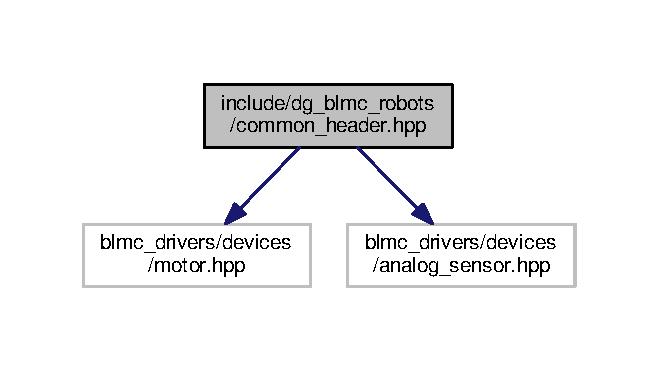
\includegraphics[width=316pt]{common__header_8hpp__incl}
\end{center}
\end{figure}
\subsection*{Typedefs}
\begin{DoxyCompactItemize}
\item 
typedef Eigen\+::\+Matrix$<$ double, 8, 1 $>$ {\bfseries blmc\+\_\+motors\+::\+Vector8d}\hypertarget{common__header_8hpp_aca38af9b287af6b2fab599056f50720a}{}\label{common__header_8hpp_aca38af9b287af6b2fab599056f50720a}

\item 
typedef std\+::shared\+\_\+ptr$<$ blmc\+\_\+drivers\+::\+Safe\+Motor $>$ {\bfseries blmc\+\_\+motors\+::\+Safe\+Motor\+\_\+ptr}\hypertarget{common__header_8hpp_a5928fcba25d1bf659f4977d91f4b3b9f}{}\label{common__header_8hpp_a5928fcba25d1bf659f4977d91f4b3b9f}

\item 
typedef std\+::shared\+\_\+ptr$<$ blmc\+\_\+drivers\+::\+Analog\+Sensor $>$ {\bfseries blmc\+\_\+motors\+::\+Slider\+\_\+ptr}\hypertarget{common__header_8hpp_a8c3b9184f8971773f9e6767e6104d28f}{}\label{common__header_8hpp_a8c3b9184f8971773f9e6767e6104d28f}

\end{DoxyCompactItemize}


\subsection{Detailed Description}
\begin{DoxyAuthor}{Author}
Manuel Wuthrich 

Maximilien Naveau 

Julian Viereck 

Johannes Pfleging 
\end{DoxyAuthor}
\begin{DoxyRefDesc}{License}
\item[\hyperlink{license__license000001}{License}]License B\+S\+D-\/3-\/\+Clause \end{DoxyRefDesc}
\begin{DoxyCopyright}{Copyright}
Copyright (c) 2019, New York University and Max Planck Gesellshaft. 
\end{DoxyCopyright}

\hypertarget{dgm__single__motor_8hpp}{}\section{include/dg\+\_\+blmc\+\_\+robots/dgm\+\_\+single\+\_\+motor.hpp File Reference}
\label{dgm__single__motor_8hpp}\index{include/dg\+\_\+blmc\+\_\+robots/dgm\+\_\+single\+\_\+motor.\+hpp@{include/dg\+\_\+blmc\+\_\+robots/dgm\+\_\+single\+\_\+motor.\+hpp}}
{\ttfamily \#include $<$dynamic\+\_\+graph\+\_\+manager/dynamic\+\_\+graph\+\_\+manager.\+hh$>$}\\*
{\ttfamily \#include $<$blmc\+\_\+robots/single\+\_\+motor.\+hpp$>$}\\*
Include dependency graph for dgm\+\_\+single\+\_\+motor.\+hpp\+:
\nopagebreak
\begin{figure}[H]
\begin{center}
\leavevmode
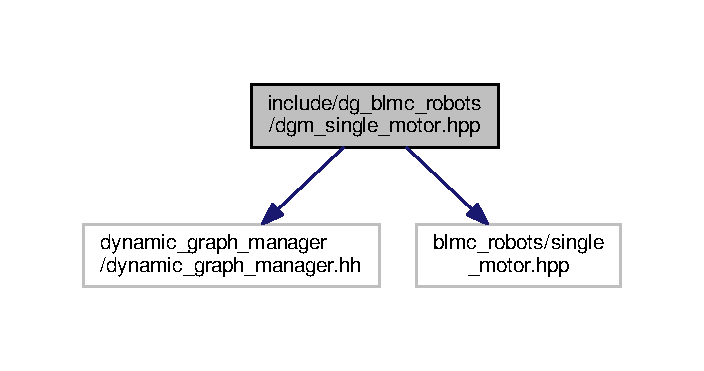
\includegraphics[width=338pt]{dgm__single__motor_8hpp__incl}
\end{center}
\end{figure}
\subsection*{Classes}
\begin{DoxyCompactItemize}
\item 
class \hyperlink{classdg__blmc__robots_1_1DGMSingleMotor}{dg\+\_\+blmc\+\_\+robots\+::\+D\+G\+M\+Single\+Motor}
\end{DoxyCompactItemize}
\subsection*{Typedefs}
\begin{DoxyCompactItemize}
\item 
typedef Eigen\+::\+Matrix$<$ double, 1, 1 $>$ {\bfseries dg\+\_\+blmc\+\_\+robots\+::\+Vector1d}\hypertarget{dgm__single__motor_8hpp_a579c47054e6fefa2135c56933d82b86c}{}\label{dgm__single__motor_8hpp_a579c47054e6fefa2135c56933d82b86c}

\end{DoxyCompactItemize}


\subsection{Detailed Description}
\begin{DoxyAuthor}{Author}
Manuel Wuthrich 

Maximilien Naveau 

Julian Viereck 

Johannes Pfleging 
\end{DoxyAuthor}
\begin{DoxyRefDesc}{License}
\item[\hyperlink{license__license000002}{License}]License B\+S\+D-\/3-\/\+Clause \end{DoxyRefDesc}
\begin{DoxyCopyright}{Copyright}
Copyright (c) 2019, New York University and Max Planck Gesellshaft. 
\end{DoxyCopyright}

\hypertarget{dgm__stuggihop_8hpp}{}\section{include/dg\+\_\+blmc\+\_\+robots/dgm\+\_\+stuggihop.hpp File Reference}
\label{dgm__stuggihop_8hpp}\index{include/dg\+\_\+blmc\+\_\+robots/dgm\+\_\+stuggihop.\+hpp@{include/dg\+\_\+blmc\+\_\+robots/dgm\+\_\+stuggihop.\+hpp}}
{\ttfamily \#include $<$dynamic\+\_\+graph\+\_\+manager/dynamic\+\_\+graph\+\_\+manager.\+hh$>$}\\*
{\ttfamily \#include $<$blmc\+\_\+robots/stuggihop.\+hpp$>$}\\*
Include dependency graph for dgm\+\_\+stuggihop.\+hpp\+:
\nopagebreak
\begin{figure}[H]
\begin{center}
\leavevmode
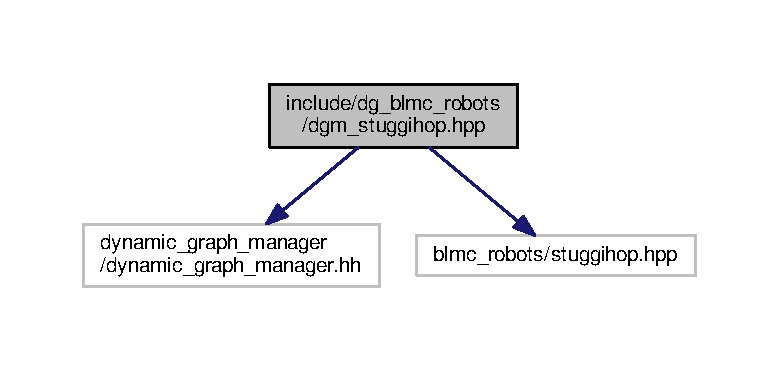
\includegraphics[width=350pt]{dgm__stuggihop_8hpp__incl}
\end{center}
\end{figure}
This graph shows which files directly or indirectly include this file\+:
\nopagebreak
\begin{figure}[H]
\begin{center}
\leavevmode
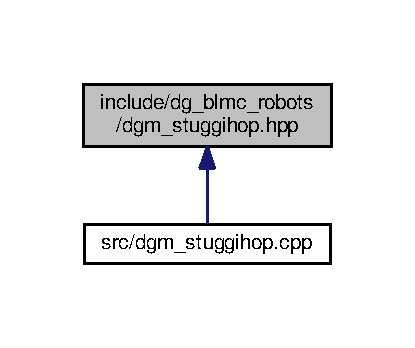
\includegraphics[width=199pt]{dgm__stuggihop_8hpp__dep__incl}
\end{center}
\end{figure}
\subsection*{Classes}
\begin{DoxyCompactItemize}
\item 
class \hyperlink{classdg__blmc__robots_1_1DGMStuggihop}{dg\+\_\+blmc\+\_\+robots\+::\+D\+G\+M\+Stuggihop}
\end{DoxyCompactItemize}


\subsection{Detailed Description}
\begin{DoxyAuthor}{Author}
Manuel Wuthrich 

Maximilien Naveau 

Julian Viereck 

Johannes Pfleging 
\end{DoxyAuthor}
\begin{DoxyRefDesc}{License}
\item[\hyperlink{license__license000007}{License}]License B\+S\+D-\/3-\/\+Clause \end{DoxyRefDesc}
\begin{DoxyCopyright}{Copyright}
Copyright (c) 2019, New York University and Max Planck Gesellshaft. 
\end{DoxyCopyright}

\hypertarget{dgm__solo__simple__simu_8cpp}{}\section{src/dgm\+\_\+solo\+\_\+simple\+\_\+simu.cpp File Reference}
\label{dgm__solo__simple__simu_8cpp}\index{src/dgm\+\_\+solo\+\_\+simple\+\_\+simu.\+cpp@{src/dgm\+\_\+solo\+\_\+simple\+\_\+simu.\+cpp}}


The hardware wrapper of the solo naive simulation.  


{\ttfamily \#include \char`\"{}dg\+\_\+blmc\+\_\+robots/dgm\+\_\+solo\+\_\+simple\+\_\+simu.\+hpp\char`\"{}}\\*
Include dependency graph for dgm\+\_\+solo\+\_\+simple\+\_\+simu.\+cpp\+:
\nopagebreak
\begin{figure}[H]
\begin{center}
\leavevmode
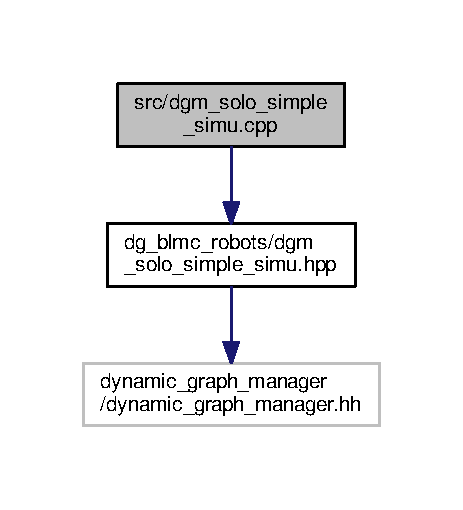
\includegraphics[width=222pt]{dgm__solo__simple__simu_8cpp__incl}
\end{center}
\end{figure}


\subsection{Detailed Description}
The hardware wrapper of the solo naive simulation. 

\begin{DoxyAuthor}{Author}
Maximilien Naveau 
\end{DoxyAuthor}
\begin{DoxyDate}{Date}
2018
\end{DoxyDate}
This file defines the D\+G\+M\+Quadruped\+Simu class. 
\hypertarget{dgm__stuggihop_8cpp}{}\section{src/dgm\+\_\+stuggihop.cpp File Reference}
\label{dgm__stuggihop_8cpp}\index{src/dgm\+\_\+stuggihop.\+cpp@{src/dgm\+\_\+stuggihop.\+cpp}}


D\+GM wrapper around the stuggihop robot.  


{\ttfamily \#include \char`\"{}dg\+\_\+blmc\+\_\+robots/dgm\+\_\+stuggihop.\+hpp\char`\"{}}\\*
Include dependency graph for dgm\+\_\+stuggihop.\+cpp\+:
\nopagebreak
\begin{figure}[H]
\begin{center}
\leavevmode
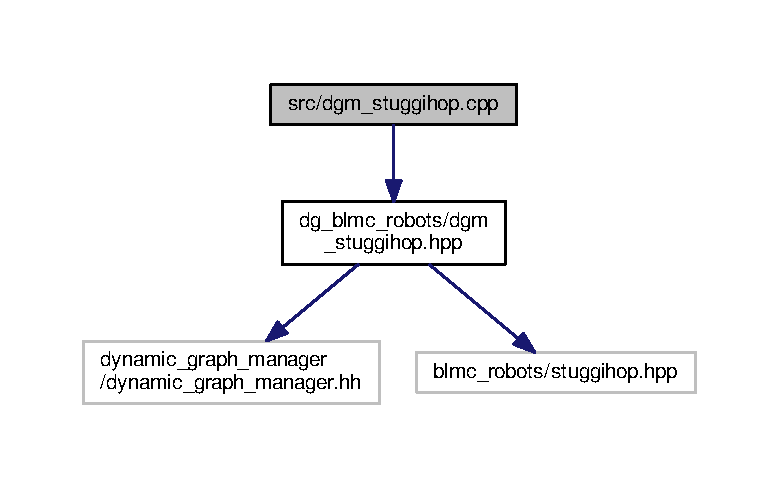
\includegraphics[width=350pt]{dgm__stuggihop_8cpp__incl}
\end{center}
\end{figure}


\subsection{Detailed Description}
D\+GM wrapper around the stuggihop robot. 

\begin{DoxyAuthor}{Author}
Steve Heim 
\end{DoxyAuthor}
\begin{DoxyDate}{Date}
2019 
\end{DoxyDate}

%--- End generated contents ---

% Index
\backmatter
\newpage
\phantomsection
\clearemptydoublepage
\addcontentsline{toc}{chapter}{Index}
\printindex

\end{document}
